\documentclass[11pt,a4paper]{article}
\usepackage[margin=1in]{geometry}
\usepackage[T1]{fontenc}
\usepackage{lmodern,amsmath,amssymb,amsthm,mathtools,microtype}
\usepackage{enumitem,booktabs,graphicx,tikz}
\usetikzlibrary{arrows.meta,positioning,calc,patterns,decorations.pathreplacing}
\usepackage[colorlinks=true,linkcolor=blue!50!black,citecolor=blue!50!black,urlcolor=blue!50!black]{hyperref}
\newtheorem{theorem}{Theorem}[section]
\newtheorem{lemma}[theorem]{Lemma}
\newtheorem{proposition}[theorem]{Proposition}
\newtheorem{corollary}[theorem]{Corollary}
\newtheorem{claim}[theorem]{Claim}
\theoremstyle{definition}
\newtheorem{definition}[theorem]{Definition}
\theoremstyle{remark}
\newtheorem{remark}[theorem]{Remark}
\newcommand{\OO}{\mathcal O}
\newcommand{\ZZ}{\mathbb Z}
\newcommand{\RR}{\mathbb R}
\newcommand{\NN}{\mathbb N}
\newcommand{\CC}{\mathbb C}
\DeclareMathOperator{\Alt}{Alt}
\DeclareMathOperator{\Sym}{Sym}
\DeclareMathOperator{\supp}{supp}
\DeclareMathOperator{\im}{im}
\DeclareMathOperator{\id}{id}
\DeclareMathOperator{\coker}{coker}
\DeclareMathOperator{\Stab}{Stab}
\DeclareMathOperator{\Hom}{Hom}
\DeclareMathOperator{\Aut}{Aut}
\DeclareMathOperator{\GL}{GL}
\newcommand{\HS}{\mathrm{HS}}
\newcommand{\TV}{\mathrm{TV}}
\hypersetup{pdftitle={An infinite finitely presented simple amenable group},pdfauthor={OpenAI}}
\title{An infinite finitely presented simple amenable group}
\author{OpenAI}
\date{September 23, 2026}
\begin{document}
\maketitle
\begin{abstract}
We construct an infinite finitely presented simple amenable group, giving a positive answer to the finite-presentation existence question for simple amenable groups.
\end{abstract}
\section{Introduction}\label{sec:introduction}

A discrete group $G$ is \emph{amenable} if, for every finite
$K\subseteq G$ and every $\varepsilon>0$, there is a nonempty finite
$D\subseteq G$ such that
\begin{equation}\label{eq:folner-introduction}
 |gD\mathbin{\triangle}D|<\varepsilon |D|
 \qquad(g\in K).
\end{equation}
It is \emph{simple} if its only normal subgroups are the trivial
group and $G$, and \emph{finitely presented} if
$G\cong F(S)/\langle\!\langle R\rangle\!\rangle$ for finite sets
of generators $S$ and relator words $R$. We address the existence
problem asking whether these three properties can hold together
in an infinite group.

\begin{theorem}\label{thm:main}
There exists an infinite finitely presented simple amenable group.
\end{theorem}

The group will be an alternating subgroup of a polygon exchange
group on a sufficiently large finite number of squares. Both the
number of squares and the eventual sets of generators and relators
are finite. No uniform bound on their sizes is needed for the
existence statement.

\subsection{Context and the role of finite presentation}

A topological full group records the finite local orbit rules of a
dynamical system.  For a homeomorphism $\varphi$ of a Cantor space,
it consists of the homeomorphisms that agree with integer powers of
$\varphi$ on the members of a finite clopen partition.  Giordano,
Putnam and Skau developed these groups as invariants of Cantor
minimal systems and their orbit equivalence relations
\cite{GiordanoPutnamSkau1999}.  Matui proved simplicity of their
derived groups and characterized finite generation by the minimal
subshift condition \cite[Theorems~4.9 and~5.4]{Matui2006}.
Juschenko and Monod then proved amenability of the full group of
every minimal homeomorphism of a Cantor space
\cite[Theorem~A]{JuschenkoMonod2013}.  Combined with this earlier
structure theory, their Corollary~B gives infinite finitely generated
simple amenable groups.

Finite presentation is the obstruction left by those examples.
The existence question predates them: Button records it in
\cite[p.~729]{Button2010}, and Juschenko and Monod raise it again
on page~776 of \cite{JuschenkoMonod2013}.
Matui proved that the derived groups arising from minimal subshifts
are not finitely presented \cite[Theorem~5.7]{Matui2006}.
Grigorchuk and Medynets established a broader approximation property:
the full group of every Cantor minimal system is locally embeddable
into finite groups \cite[Theorem~2.6]{GrigorchukMedynets2014}.
This means that each finite subset admits an injective map into a
finite group preserving all products that stay within that subset.
The property passes to subgroups, and a finitely presented group
with this property is residually finite.  An infinite simple group
cannot be residually finite, since a nontrivial homomorphism from
it to a finite group would be injective.  Thus this local finite
approximation property also explains why the classical full-group
examples cannot settle the finite-presentation question.

There is also a presentation theory for the classical examples.
Grigorchuk and Medynets describe their derived groups using local
$3$-cycles and relations expressing refinement and disjointness of
clopen pieces \cite{GrigorchukMedynets2018}. For a minimal subshift,
their presentation can use a finite generating set, but its relations
remain infinitely indexed. Such presentations separate the task of
finding finite generators from the harder task of deriving all local
permutation laws from finitely many relations.

Subsequent constructions have strengthened the finitely generated
existence theorem in other directions. Nekrashevych constructed
infinite finitely generated simple torsion groups of intermediate
growth \cite[Theorem~1.2]{Nekrashevych2018}, and Kionke and Schesler
obtained two-generated infinite simple amenable groups
\cite{KionkeSchesler2024}. These advances do not give finite
presentation. The latter requirement still appears in Zaremsky's
July 2026 problem list \cite[Problem~10]{Zaremsky2026};
Theorem~\ref{thm:main} answers the existence question positively.

Higher-dimensional piecewise translation groups offer a broader
setting, but bring a separate amenability problem.  Chornyi,
Juschenko and Nekrashevych extended finite-generation methods to
the derived subgroups of full groups of minimal faithful $\ZZ^d$-actions
conjugate to finite-alphabet subshifts
\cite[Theorem~1 in the author version]{ChornyiJuschenkoNekrashevych2020}.
Nekrashevych's alternating full groups organize the local even
permutations through multisections, and their simplicity follows
from minimality for effective {\'e}tale groupoids with Cantor unit space
\cite[Section~3 and Theorem~4.1]{Nekrashevych2019}.
Our local even permutations are an instance of that construction; we
prove the needed comparison and simplicity statements directly.
Amenability does not follow from the rank of the acting group:
Elek and Monod constructed a free minimal Cantor $\ZZ^2$-action
whose full group contains a nonabelian free group
\cite[Theorem~1]{ElekMonod2013}.

The geometric construction has a particularly close predecessor
in the Penrose model of Chornyi, Juschenko and Nekrashevych
\cite[Section~4 in the author version]{ChornyiJuschenkoNekrashevych2020}.
They split the plane along five arithmetic families of lines, realize
polygonal pieces as clopen sets, and describe the full group by
piecewise translations on four pentagonal windows. The translation
group has rank four over $\ZZ$. Our model likewise combines a split
plane with finitely many polygonal regions, but uses four directions
over a real quadratic ring. Amenability requires a separate argument:
the Penrose example in that source is not asserted to be amenable.

Cornulier and Lacourte study the unrestricted rectangle exchange
group on $[0,1)^d$, for every $d\geq1$, allowing arbitrary real
endpoints and translation vectors \cite{CornulierLacourte2025}.
They prove that its derived subgroup is simple and ask about
amenability, second homology, and bounded relator length over the
infinite generating set of all restricted shuffles. Our group
restricts the arithmetic parameters and permits two inclined edge
directions in addition to the coordinate directions. Finite unions
of coordinate rectangles do not give these inclined boundaries.
Moreover, bounded relator length over an infinite set of generators
is a different requirement from the finite presentation sought here.
The proof below propagates relations while keeping the generating
set fixed and finite.

The amenability argument is related to the almost-invariant finite
configurations of Juschenko and Monod
\cite[Theorem~C]{JuschenkoMonod2013} and to the extensive-amenability
methods of Juschenko, Matte Bon, Monod and de la Salle
\cite[Section~5]{JuschenkoMatteBonMonodDeLaSalle2018}.
For interval-exchange groups whose translation increments modulo
one generate an abelian group of rational rank at most two,
recurrence gives an extensively amenable action on the circle.
Comparing the two continuity conventions at discontinuities gives
a cocycle into finitely supported permutations with amenable
kernel. Polygonal boundaries
are line segments, so this finite-discontinuity argument does not
apply directly. Here correlated random fields produce polygonal
partitions whose barriers respect every prescribed translation
chart. Matching cells of the same shape then yields almost-invariant
measures on the exchange group.

The homological argument follows the stability and symmetric
monoidal category approach used by Szymik and Wahl for
Higman--Thompson groups \cite{SzymikWahl2019}. Li's general
framework also reaches individual full groups and their derived
groups: for minimal ample groupoids with locally compact Hausdorff
unit space, no isolated units, and comparison, their homology is
identified with that of an infinite loop space and its universal
cover, respectively \cite[Theorem~5.18 and Corollary~5.20]{Li2025}.
We give a concrete low-degree implementation for the polygon
algebra. An explicit resolution reduces the calculation to
translation modules of polygonal step functions, and a fixed
finite collection of square copies controls the passage to the alternating
group's multiplier. Polyhedral indicator modules and finite
translation-orbit data also underlie the projection-pattern
calculations recalled in
\cite[Section~3.1]{GahlerHuntonKellendonk2013}; our coefficient
finiteness is proved directly by corner data. We use
Segal's bar and realization results and
ordinary integral group completion, with the corrected proof of
Miller and Palmer
\cite{Segal1974,McDuffSegal1976,MillerPalmer2015}.

\subsection{The construction and the proof}

The polygons have edges on level lines of
\[
 x,\quad y,\quad y-\lambda x,\quad x-\lambda y,
\]
at levels in $\OO=\ZZ[\tau]$, where $\tau=(1+\sqrt5)/2$ and
$\lambda$ is a sufficiently large power of $\tau$. The other real
embedding makes $\lambda$ small. We identify polygonal sets that
differ only on their edges, or equivalently use the compact Stone
space $X$ of their Boolean algebra on a square. For a finite
integer $m$, the group $F_m$ consists of all finite piecewise
translations of $m$ disjoint copies of $X$. Its subgroup $A_m$ is
generated by even permutations of disjoint translated polygonal
pieces, with the pieces identified by their translations.
These definitions are made precise in Section~\ref{sec:geometry}.
We eventually choose one finite $m$ satisfying all homology and
local-permutation requirements, and use that same $A_m$ for every
property.  The homological stabilization below is a tool for studying
this fixed group; the example is not a union over increasing track
numbers.

Strict area comparison supplies spare pieces. It implies that
$A_m=[F_m,F_m]$ is infinite, perfect, and simple
(Theorem~\ref{thm:simplicity}). The remaining proof has three parts.
\begin{enumerate}[leftmargin=*,label=\textup{\arabic*.}]
\item \emph{Amenability.}
For a fixed finite collection of exchanges, we build partition
boundaries from marked segments on allowable lines. One random
field selects subdivision points on each line, and a second
selects the segments between them. The fields are correlated over
a range of scales in the conjugate embedding. The correlations make
bounded translations inexpensive in total variation while keeping
individual fluctuations small. Prescribed mean values force the
chart-edge intersections to be marked and the chart boundaries
to be barriers on an event of arbitrarily high probability.
On that event every partition cell stays in a translation chart,
so its image has the same shape. Uniform matchings between cells
of the same shape convert the partition laws into finitely
supported almost invariant group measures, and then into the
F\o lner sets in
\eqref{eq:folner-introduction}
(Theorem~\ref{thm:amenability}).

\item \emph{Finite generation of the multiplier.}
We prove that the Schur multiplier $H_2(A_m;\ZZ)$ is finitely
generated once $m$ is sufficiently large. An ordered-embedding complex gives homological
stability for $F_m$ in the needed degrees. A symmetric monoidal
category of polygons then reduces its stable homology to translation
homology of integer-valued polygonal functions. Such functions are
detected by finitely many translation types of corner data, giving
the required algebraic finiteness. An argument using a fixed finite
bank of reserved tracks transfers the result to $A_m$ (Theorem~\ref{thm:multiplier}).

\item \emph{A finitely presented central cover.}
We use permutations of the tracks applied only over specified
polygonal sets, together with translations whose total shift over
the tracks is zero. Finitely many such elements generate $A_m$.
A finite collection of their true relations presents a group
$\widehat G$ mapping onto $A_m$; the task is to prove that the
kernel is central.

Start with the permutation relations for coordinate cuts at
$i\tau$ modulo one, with $i$ ranging over a fixed finite interval
of integers. To extend this
range, the large ordinary slope of $\lambda$ places an inclined
line between two small coordinate rectangles. Its small conjugate
value keeps the new transverse coordinate indices within ranges covered
by the preceding induction step. Fixed overlap relations compare
the permutation actions along that line, proving that permutations
on the two rectangles commute. This enlarges the coordinate laws.
The resulting rectangular decompositions then reduce arbitrary
polygonal tests to finitely many configurations of concurrent lines.
Finally, exact conjugation formulas for permutations of disjoint
translated pieces show that a word acting trivially on the $m$ squares
commutes with every
generator of $\widehat G$ (Theorem~\ref{thm:central-cover}).
\end{enumerate}

The last two parts have different purposes. A finitely generated
second homology group alone does not imply finite presentation.
Together with the central extension
\[
 1\longrightarrow K\longrightarrow\widehat G
 \longrightarrow A_m\longrightarrow1,
\]
the homological five-term sequence shows that $K$ is a finitely
generated abelian group. Killing finitely many generators of $K$
then gives a finite presentation of $A_m$.

Sections~\ref{sec:geometry}--\ref{sec:simplicity} construct the group
and establish simplicity. Sections~\ref{sec:amenability}
and~\ref{sec:homology} prove the first two main ingredients.
Sections~\ref{sec:lifting}--\ref{sec:transport} construct the central
cover, and Section~\ref{sec:conclusion} completes the proof of
Theorem~\ref{thm:main}.

\section{The polygon algebra and its translation groups}\label{sec:geometry}

We first construct the group to which the three main arguments will apply.
Four families of parallel cuts will be used. Two are coordinate cuts; the
other two allow local relations to propagate between widely separated
coordinate cuts.

\subsection{A quadratic ring and four directions}

Put
\[
 \tau=\frac{1+\sqrt5}{2},\qquad \OO=\ZZ[\tau].
\]
The conjugate embedding sends $\tau$ to $\bar\tau=(1-\sqrt5)/2$;
a bar on a vector means conjugation in each coordinate. The unit $\tau$
satisfies $|\bar\tau|=\tau^{-1}$. Choose a positive integer $a$, to be
fixed below, and put $\lambda=\tau^a$. Our four linear forms are
\begin{equation}\label{eq:four-forms}
 \ell_1(x,y)=x,\quad \ell_2(x,y)=y,\quad
 \ell_3(x,y)=y-\lambda x,\quad
 \ell_4(x,y)=x-\lambda y.
\end{equation}
An \emph{allowable line} is $\ell_i^{-1}(t)$ with $t\in\OO$.
Translations by $\OO^2$ preserve these four line families.

\begin{lemma}[Arithmetic of the cuts]\label{lem:arithmetic}
The following statements hold.
\begin{enumerate}[label=\textup{(\roman*)}]
\item There is a positive integer $D$, depending only on $\lambda$, such
that every intersection of nonparallel allowable lines lies in
$D^{-1}\OO^2$. There are finitely many such vertex types modulo
$\OO^2$, including the set of allowable directions through the vertex.
Each type has representatives arbitrarily close to the origin.
\item In each allowable line direction, the group of translations in
$\OO^2$ parallel to that line is dense in the line and has a pair of
generators of arbitrarily small ordinary length.
\item The image of $\OO$ under $z\mapsto(z,\bar z)$ is a lattice in
$\RR^2$. There are absolute constants $C,c>0$ such that, for every
integer $n\ge1$ and every interval $J$ of $n$ consecutive integers,
the points
$\{i\tau\bmod1:i\in J\}$ have largest circular gap at most $C/n$;
any two distinct points in this set have circular distance at least
$c/n$.
\end{enumerate}
\end{lemma}

\begin{proof}
The coefficient determinants of pairs in \eqref{eq:four-forms} belong,
up to sign, to $\{1,\lambda,1-\lambda^2\}$. The first two are units in
$\OO$. Since the reciprocal of a nonzero algebraic integer $v$ is
$\bar v/N(v)$, a common positive integer denominator gives the asserted
$D$. The group $D^{-1}\OO^2/\OO^2$ is finite. Moreover, whether
$\ell_i(v)$ belongs to $\OO$ depends only on this residue class, so
the directions through a vertex introduce no additional infinite
choice. Every coset has dense ordinary image because $\OO^2$ does.

For the coordinate directions the tangent translation groups have
bases $(1,0),(\tau,0)$ and $(0,1),(0,\tau)$. For the other directions
they have bases
\[
 (1,\lambda),\ \tau(1,\lambda)
 \quad\hbox{and}\quad
 (\lambda,1),\ \tau(\lambda,1).
\]
Multiplying both basis vectors by the unit $\tau^{-b}$ leaves the
group unchanged and makes their ordinary lengths as small as desired.

The two vectors $(1,1)$ and $(\tau,\bar\tau)$ generate the stated
lattice, since their determinant is $-\sqrt5$. Multiplication by
$\tau^k$ acts on the two factors with absolute scale factors
$\tau^k$ and $\tau^{-k}$. A fixed lattice covering radius, followed
by such a rescaling, therefore gives a constant $C_0$ with this
property: every axis-parallel rectangle of sufficiently large fixed
area and side lengths comparable to $L^{-1},L$, for $L\ge1$, meets
the lattice. More explicitly, start with a square containing a
translate of a fundamental parallelogram around every point, and
rescale by a unit with $\tau^k$ within a factor $\tau$ of $L$;
increasing one absolute constant absorbs this bounded factor.

Apply this observation with $L$ a small fixed multiple of $n$.
For any chosen ordinary coordinate $t\in[0,1]$, center the long
conjugate interval so that
\[
 i=\frac{z-\bar z}{\tau-\bar\tau}
\]
falls in the middle half of $J$. A conjugate interval of length a
fixed small multiple of $n$, and an ordinary interval of length
$C_1/n$ about $t$, then produce $z=k+i\tau$ with $i\in J$ and
$|z-t|\le C_1/n$. Constants may be enlarged to cover the bounded
small values of $n$. Thus these circular points form a
$C_1/n$-net, which proves the gap bound with $C=2C_1$.

For separation, choose the representative
$z=k+(i-j)\tau$ of a nonzero circular difference with $|z|\le1/2$.
It is a nonzero algebraic integer and
$|\bar z|=|z-(i-j)\sqrt5|\le\sqrt5 n+1/2$.
Consequently
\[
 1\le |N(z)|=|z\bar z|
 \le |z|(\sqrt5 n+1/2).
\]
Taking, for example, $c=(\sqrt5+1)^{-1}$ proves the claim.
\end{proof}

Fix $a$ sufficiently large that
\begin{equation}\label{eq:lambda-choice}
 \lambda c>1000(C+1),\qquad |\bar\lambda|<1/1000.
\end{equation}
This choice is possible because the two embeddings of $\tau^a$ have
reciprocal absolute values. All constants below may depend on this
fixed choice. The two-dimensional version of the lattice statement
is obtained by taking a product: $(z,\bar z)$ for $z\in\OO^2$ is a
lattice in $\RR^4$ with the same simultaneous rescaling property.

\subsection{Boolean polygons and the Stone space}

Consider the Boolean algebra generated by the half-planes bounded by
allowable lines, restricted to a unit square, with opposite sides
identified when applying translations. Two polygonal descriptions are
identified if they differ only on finitely many allowable line
segments. Equivalently, evaluate all descriptions on points avoiding
every allowable line. A nonzero element then has nonempty ordinary
interior. We call its elements \emph{Boolean polygons}; they include
finite unions and complements of ordinary polygonal pieces.

This convention avoids choosing a preferred value at a cut. It can
also be made into an ordinary compact topological space. Let $X$ be
the Stone space of this countable Boolean algebra: its points are
ultrafilters and its clopen sets correspond exactly to Boolean
polygons. The algebra has no atoms, since every region of nonempty
interior can be split by an allowable coordinate cut. Hence $X$ is a
compact metrizable space without isolated points. We continue to
write a polygon $U$ for its associated clopen subset of $X$.
Lebesgue area defines a finitely additive measure $\mu$ on these
sets, with $\mu(X)=1$ and $\mu(U)>0$ whenever $U\ne\varnothing$.

An analogous cut-space realization appears in the Penrose-tiling
full-group construction of
\cite[Section~4 in the author version]{ChornyiJuschenkoNekrashevych2020}:
splitting along line families gives a zero-dimensional space with polygonal
clopen sets.  Here the four line families and their quadratic translation
ring are the ones specified above.

The group
\[
 \Gamma=(\OO/\ZZ)^2\cong\ZZ^2
\]
acts on $X$ by translation modulo one. To see explicitly that this
action is free, use successively finer coordinate rectangles to
associate to every ultrafilter its unique ordinary location in
$\RR^2/\ZZ^2$. This gives a continuous equivariant map from $X$ to
the ordinary torus. A nonzero element of $\Gamma$ has no fixed point
on that torus, and therefore has no fixed point on $X$. The density
of $\Gamma$ on the torus also shows that every orbit meets every
nonempty Boolean polygon: move the ordinary location into its
interior.

All partitions and maps used below have finite descriptions. In
particular, compactness is invoked only to pass from a clopen cover
to a finite clopen partition; it does not permit countably piecewise
group elements.

\subsection{Tracks, translation tables, and slots}

For a positive integer $m$, write $mX=\{1,\ldots,m\}\times X$ and
call its copies of $X$ \emph{tracks}. Extend $\mu$ additively, so
$\mu(mX)=m$. Define $F_m$ to consist of all bijections of $mX$ that
have a finite clopen partition on whose pieces they take the form
\begin{equation}\label{eq:translation-table}
 (i,x)\longmapsto(j,x+\gamma),\qquad \gamma\in\Gamma.
\end{equation}
These maps form a countable group and preserve $\mu$.

Let $U$ be a nonempty Boolean polygon. A \emph{slot with parameter
set $U$} is an embedding $e:U\longrightarrow mX$ given by finitely
many translations and track changes. These slots give the local multisections used to define alternating
full groups in \cite[Section~3]{Nekrashevych2019}.  A collection
$e_1,\ldots,e_r$ of such embeddings with disjoint images realizes
every $\sigma\in\Sym(r)$ as a group element that sends
$e_i(x)$ to $e_{\sigma(i)}(x)$ and fixes the complement. The subgroup
$A_m\le F_m$ is generated by these elements for
$\sigma\in\Alt(r)$, over all finite disjoint slot collections.
It suffices to use three slots and a $3$-cycle, since these generate
each finite alternating group. It also suffices to require each
individual slot to be an ordinary translated copy in a single track:
refine $U$ until all the finitely many embeddings have the form
\eqref{eq:translation-table}, and multiply the resulting permutations
on disjoint pieces.

The allowance of piecewise embeddings makes $A_m$ visibly normal in
$F_m$: conjugation simply composes each slot embedding with an
element of $F_m$. Section~\ref{sec:simplicity} proves that this
alternating subgroup is the desired infinite simple group. The rest
of the paper establishes its two harder properties, amenability and
finite presentation, after a sufficiently large finite $m$ has been
chosen.

\section{Comparison, perfection, and simplicity}\label{sec:simplicity}

The area measure supplies room for extra slots. The strict inequality
in the following comparison statement is essential; no assertion
about arbitrary equal-area polygons is needed.

\begin{lemma}[Strict comparison]\label{lem:comparison}
If $U,V\subseteq mX$ are Boolean polygons and $\mu(U)<\mu(V)$,
then $U$ has a piecewise translation embedding into $V$.
\end{lemma}

\begin{proof}
Use coordinate squares of side $\varepsilon=\tau^{-b}\in\OO$,
with all grid lines allowable. Subdivide representatives of $U$
by this grid. The number of grid squares meeting their interiors is
\[
 \mu(U)\varepsilon^{-2}+O(\varepsilon^{-1}),
\]
whereas the number of whole grid squares contained in the interiors
of representatives of $V$ is
\[
 \mu(V)\varepsilon^{-2}-O(\varepsilon^{-1}).
\]
The error estimates follow by covering the finitely many polygonal
boundary segments with $O(\varepsilon^{-1})$ grid squares. They are
unchanged when summed over tracks. For sufficiently large $b$, the
second number exceeds the first. Inject the source grid squares into
the destination squares, translating the portion of $U$ in each
source square into the assigned square. The translations are in
$\OO^2$. Boundary ambiguities disappear in the Boolean algebra.
\end{proof}

\begin{lemma}[Alternating extension]\label{lem:extension}
Let $B,U,V\subseteq mX$ be Boolean polygons with $U,V$ disjoint
from $B$. Suppose $f:U\to V$ is a piecewise translation bijection
and
\[
 10\mu(U)<\mu(mX\setminus B).
\]
There is $a\in A_m$ agreeing with $f$ on $U$ and fixing $B$
pointwise. The assertion includes the empty case $U=\varnothing$.
\end{lemma}

\begin{proof}
Assume $t=\mu(U)>0$. By Lemma~\ref{lem:comparison}, choose three
pairwise disjoint copies $W_1,W_2,W_3$ of $U$ outside $B\cup U\cup V$.
At each choice the remaining area is larger than $t$: even after
removing $U,V$ and two such copies, it exceeds $6t$.
Identify the three $W_i$ with $U$ by the chosen piecewise embeddings.
The $3$-cycle on $(U,W_1,W_2)$ sends $U$ to $W_1$.
The $3$-cycle on $(W_1,V,W_3)$, using $f$ for the identification with
$V$, sends $W_1$ to $V$ with the prescribed parameters. Their product,
with the first cycle applied first, agrees with $f$ on $U$.
All participating slots avoid $B$.
\end{proof}

The same proof applies inside any permitted clopen region, with its
area in place of $m$. In particular, if a piecewise bijection is
specified on a bank of $q$ tracks, it extends to an element of $A_m$
whenever $m>10q$. This quantitative observation will be used for the
finite-track homology argument.

The proof below uses the supported double-commutator method for
alternating full groups \cite[Theorem~4.1 and its proof]{Nekrashevych2019}.
Strict area comparison supplies the small translated copies needed
to carry that argument out in our polygon algebra.

\begin{theorem}\label{thm:simplicity}
For every positive integer $m$, the group $A_m$ is infinite, perfect,
and simple, and
\[
 [F_m,F_m]=A_m.
\]
\end{theorem}

\begin{proof}
We first show that every coset of $A_m$ in $F_m$ has a representative
with arbitrarily small support. Fix $f\in F_m$ and $\delta>0$.
Subdivide $mX$ into finitely many pieces of area less than
$\delta/20$. Suppose a representative of $fA_m$ has already been
made the identity on a clopen union $B$. If its remaining region has
area at least $\delta$, choose one of the small pieces $U$ outside
$B$. Its image $V$ also avoids $B$. Apply
Lemma~\ref{lem:extension} to the inverse of its restriction from
$U$ to $V$, keeping $B$ fixed. Composing on the left fixes $U$ as
well as $B$. Because the partition is finite, this process either
fixes the entire space or leaves a support of area below $\delta$.
Normality of $A_m$ ensures that all the representatives stay in the
same coset.

Given $f,g\in F_m$, choose small-support representatives $f_0,g_0$
of their cosets. Lemmas~\ref{lem:comparison} and
\ref{lem:extension} allow the support of $g_0$ to be moved off the
support of $f_0$ by conjugation in $A_m$. More explicitly, choose
both supports of area less than $m/100$, embed the second into the
complement of the first, and extend that embedding. The resulting
representatives commute. Therefore $F_m/A_m$ is abelian and
$[F_m,F_m]\subseteq A_m$.

For the reverse inclusion and perfection, consider an alternating
slot permutation and subdivide its parameter set into sufficiently
small pieces. Each resulting permutation can be included in a finite
alternating slot group with at least five slots, by adding spare
copies using strict comparison. The finite group $\Alt(r)$ is
perfect for $r\ge5$: every $3$-cycle is a commutator of even
permutations on five letters, since the commutator of
$(1\,2)(4\,5)$ and $(2\,3)(4\,5)$ is a $3$-cycle (or its inverse,
according to the commutator convention). Thus every generating
slot permutation is a product of commutators within $A_m$.
Consequently $A_m=[A_m,A_m]\subseteq[F_m,F_m]$.

Arbitrarily many sufficiently small translated squares fit disjointly
inside one track. Their alternating permutations embed $\Alt(r)$
in $A_m$ for arbitrarily large $r$, so $A_m$ is infinite.

Finally, let $N\lhd A_m$ contain a nonidentity element $n$.
There is a nonempty clopen $U$ with $U\cap nU=\varnothing$:
choose a point moved by $n$ and disjoint clopen neighborhoods of it
and its image, then shrink the first neighborhood. For $a,b\in A_m$
supported in $U$, the element $nan^{-1}$ is supported in $nU$ and
commutes with both. With $[s,t]=sts^{-1}t^{-1}$ we obtain
\[
 [[n,a],b]=[a^{-1},b]\in N.
\]
It follows that $N$ contains the commutator subgroup of the subgroup
of $A_m$ supported in $U$.

Take any generating $3$-cycle of slots and subdivide its parameter
set until the area of each piece is less than
$\min\{\mu(U)/10,m/100\}$. For each such piece add two spare
slots, obtaining a five-slot alternating group whose total support
has area less than $\mu(U)$ and less than $m/10$.
Lemma~\ref{lem:comparison} embeds this support into $U$, and
Lemma~\ref{lem:extension} extends the embedding to conjugation by
an element of $A_m$. The conjugate five-slot group is perfect and
supported in $U$, so it lies in $N$ by the double commutator
calculation. Normality of $N$ brings back the original $3$-cycle
on that parameter piece. Multiplying over the subdivision shows
that every generator of $A_m$ belongs to $N$. Hence $N=A_m$.
\end{proof}

\section{Amenability from random polygonal partitions}\label{sec:amenability}

The input to this section is the polygonal Boolean algebra and its translation
arithmetic from Lemma~\ref{lem:arithmetic}.  We prove amenability for every
fixed finite number of tracks.  The main construction is a random finite
polygonal partition: with high probability its cells lie inside the translation
charts of prescribed exchanges, and its law is almost unchanged when they move the
cells.  We state the precise coupling target below, before constructing the
random fields that will supply its partition edges.

The use of almost-invariant finite configurations is related to
\cite[Theorem~C]{JuschenkoMonod2013} and the extensive-amenability
methods of \cite{JuschenkoMatteBonMonodDeLaSalle2018}.  The proof here
constructs the correlated partition law and its conversion to group
measures directly.  This is essential in dimension two, where even
free minimal Cantor $\ZZ^2$-actions can have nonamenable full
groups \cite[Theorem~1]{ElekMonod2013}.

\begin{theorem}\label{thm:amenability}
For every positive integer $m$, the discrete group $F_m$ is amenable.  Every
subgroup of $F_m$, in particular $A_m$, satisfies the finite-set F\o lner
condition.
\end{theorem}

Throughout the proof $m$ and a finite set $\mathcal K\subset F_m$ are fixed.
Include inverses in $\mathcal K$ if necessary.  Choose finite polygonal
continuity partitions for its elements, so that each piece is translated by
one vector in $\OO^2$ to a specified track.  Subdivide further along supporting
lines to obtain convex pieces.  All source and image boundaries are contained
in a fixed finite collection of allowable line segments.  Integer translations
used to cross the edges of the square are included among the translation
vectors.  Consequently their coordinates and conjugate coordinates, and the
levels and conjugate levels of all these supporting lines, are bounded by a
constant depending only on $\mathcal K$.

For each $\delta>0$ we will construct a law on finite polygonal partitions
with the following property.  For every $g\in\mathcal K$, two partitions
$\mathcal P,\mathcal P'$ with this law can be coupled so that, with
probability greater than $1-\delta$, every cell of $\mathcal P$ lies in
one translation chart of $g$ and
\[
 \mathcal P'=g\mathcal P=\{gC:C\in\mathcal P\}.
\]
Each cell is contained in a single track.  Two cells have the same shape
if they differ by an ordinary $\OO^2$ translation, ignoring their tracks.
On the displayed event, $g$ preserves the multiset of cell shapes.
For each occurring multiset, fix a baseline partition.  Uniformly matching
its cells to the sampled cells of the same shape will lift this coupling
to almost-invariant probability measures on $F_m$.  The last subsection
proves that lift and its conversion to finite F\o lner sets.

\subsection{Lattice counts and sites with a specified side}

Let $D$ be as in Lemma~\ref{lem:arithmetic}, and set
\[
 L=D^{-1}\OO^2,
 \qquad
 \Lambda=\{(z,\bar z):z\in L\}\subset\RR^2\times\RR^2.
\]
Write $\rho$ for the density of this four-dimensional lattice.  Norms on the
ordinary and conjugate planes may be taken to be the maximum norm; replacing
them by Euclidean norms changes only constants.

We record the quantitative consequences of unit rescaling that will be used.
For intervals $I,J\subset\RR$ of lengths $a,b>0$,
\begin{equation}\label{eq:am-one-count}
 \#\{u\in D^{-1}\OO:u\in I,\ \bar u\in J\}\le C(ab+1).
\end{equation}
To prove this when $ab\ge1$, rescale by a power of the unit $\tau$ so that
the two side lengths become comparable to $\sqrt{ab}$.  A fixed fundamental
parallelogram then gives the bound by counting tiles meeting the rectangle.
When $ab<1$, either the same argument applies after enlarging the rectangle
to area one, or one uses
$|u\bar u|\ge D^{-2}$ for a nonzero difference $u$ and subdivides the
rectangle into a fixed number of smaller rectangles.  This also proves that
the constant is independent of the positions of $I,J$.

There is a corresponding uniform Riemann-sum statement.  For ordinary scale
$s>0$ and conjugate scale $t>0$, the lattice in coordinates $(z/s,\bar z/t)$
has fundamental tiles of diameter at most
\begin{equation}\label{eq:am-tile}
 C(st)^{-1/2}.
\end{equation}
Indeed, apply a unit with ordinary size comparable to $\sqrt{s/t}$ to a
fixed basis of $\Lambda$ before scaling the two coordinates.  Both parts of
each resulting basis vector have size $O((st)^{-1/2})$.  The tile volume is
$1/(\rho s^2t^2)$.  If $st\to\infty$, integrating a compactly supported
Lipschitz function over these tiles and replacing its value by the value at
the lattice point changes the normalized sum by
$O((st)^{-1/2})$, uniformly over translates of the lattice.  Tiles meeting
the boundary of a fixed box contribute the same order of error.  Thus, in
particular, a box of ordinary side lengths $O(s)$ and conjugate side lengths
$O(t)$ contains $O(s^2t^2)$ sites once $st\ge1$.

At a point on a cut, a side must be specified.  Fix vectors $v,w\in\RR^2$
such that $v\ne0$ and $\ell_j(w)\ne0$ whenever $\ell_j(v)=0$.  The
\emph{flag} $(v,w)$ assigns the sign of $\ell_j-c$ at $z$ to be the
lexicographic sign of
\[
 (\ell_j(z)-c,\ell_j(v),\ell_j(w)).
\]
This is a formal convention, denoted $z+\varepsilon v+\varepsilon^2w$;
no common numerical choice of $\varepsilon$ for the infinitely many cuts is
intended.  Each Boolean polygon has a well-defined value at this flag.
On the torus, represent a flagged point by the unique lift in the closed
square whose flag enters the square.  For a fixed flag type, let $\mathcal S$
be the countable set of these representatives in the $m$ tracks with base
point in $L$ modulo $\ZZ^2$.  Each exchange permutes $\mathcal S$: use the
translation belonging to the Boolean chart selected by the flag, and then
choose the square representative again.  The inverse exchange proves
bijectivity.  Translation leaves the two flag vectors unchanged.

All subsequent field estimates hold for any one fixed flag type, with
constants allowed to depend on that type.  A finite number of independent
copies, also with different flag types, will be used for the four directions.
Boundary representatives affect none of the counts: along a fixed allowable
line in a bounded ordinary region and a conjugate ball of radius $N$, there
are $O(N)$ sites, by~\eqref{eq:am-one-count} in a tangent coordinate.

The partitions will use two bit fields for each of the four line directions.
On a finite collection of allowable line segments in the squares, the first
field marks subdivision points.  The second field decides whether the
interval beginning at each marked point is a barrier.  Together with the
square edges, these barriers cut each track into polygonal cells.  An
interval uses the second bit at its initial endpoint, interpreted by a flag
pointing along the interval into its chart.  Its terminal endpoint will be
forced independently when it lies on a chart edge.  This is why we use
tangent flags.  The exact rule, including the square endpoints, and its
covariance verification follow the field estimates.

The joint law of these fields must change little under each exchange in
$\mathcal K$.  At the same time, they must force prescribed bits at all
relevant sites: chart crossings are subdivision points, chart edges are
complete barriers, and sufficiently distant sites in the conjugate plane
are unmarked.  We next construct general fields with these two properties;
the specific fields for the partition will then be chosen from the fixed
chart data.

\subsection{Positive averaging matrices}

Let $\theta:\RR^2\to\RR$ be smooth and constant outside a compact set.
Choose $\chi\in C_c^\infty(\RR^2)$ with $0\le\chi\le1$ that equals one
on a fixed neighborhood of $\supp\nabla\theta$.  We can enlarge this
neighborhood whenever finitely many signals are being treated.  The mean
field is
\[
 \mu_N(z)=\theta(\bar z/N),
\]
with the same signal on every track.  Fix small positive parameters
$\eta,\kappa$, with $4\eta$ less than the width of the neighborhood where
$\chi=1$.  Eventually $\eta,\kappa$ will be chosen first and $N$ will then
tend to infinity.

We will construct a positive semidefinite matrix $B_N$ with finitely many
nonzero rows and columns.  We add bounded independent centered noise $\xi_z$
and a correlated perturbation $B_N\xi$ to the mean, then take the sign of
the resulting field.  A bounded chart translation changes $\mu_N$ by $O(N^{-1})$ on
$O(N^2)$ sites, so the $\ell^2$ norm of the mean difference need not tend
to zero.  The matrix $B_N$ is designed to multiply
this slowly varying difference approximately by a factor tending to
infinity.  Applying $(I+B_N)^{-1}$ will therefore make the mean difference
small in $\ell^2$, as needed for the total-variation estimate below.
Meanwhile, the $\ell^2$ norms of the rows of $B_N$ will be
sufficiently small that $\|B_N\xi\|_\infty\le1/2$ with probability tending
to one.  These are compatible demands: averaging preserves a slowly
varying signal while cancelling independent centered noise.

Let $\mathcal R_N$ be the powers of two between $N^{1/4}$ and $N^{1/2}$.
For $r\in\mathcal R_N$ put $s=r/N$ and
\[
 K(u)=(1-|u_1|)_+(1-|u_2|)_+.
\]
The lines in the next definition are auxiliary separators for the averaging
matrix.  We average over their thresholds to obtain a deterministic matrix;
the partition barriers will instead be sampled from the bit fields.  The
auxiliary separators suppress matrix entries across chart edges while
retaining averaging at most sites.

Independently for each of the four direction families choose a threshold
uniformly in $[\kappa/s,2\kappa/s]$, and cut the plane along all lines
$\ell_j=c$, $c\in\OO$, with $|\bar c|$ at most that threshold.
There are only finitely many such lines in any bounded ordinary region,
by~\eqref{eq:am-one-count}.  The flags determine on which side a site lies.
Let $P_r(z,w)$ be the probability that no chosen line separates the two
flagged sites.  This definition is used for sites on the same track.

Define a matrix, zero between different tracks, by
\begin{equation}\label{eq:am-matrix}
 M_r(z,w)=
 \frac{\chi(\bar z/N)\chi(\bar w/N)}{\rho(r\eta)^2}
 K\left(\frac{z-w}{s}\right)
 K\left(\frac{\bar z-\bar w}{N\eta}\right)P_r(z,w).
\end{equation}
Only $O(N^2)$ rows or columns can be nonzero.  This follows by applying the
box count to the bounded ordinary square and a conjugate ball of radius
$O(N)$.  Every $M_r$ is positive semidefinite.  Indeed,
$(1-|u|)_+$ is the overlap length of two translates of a unit interval, so
its convolution kernel is positive semidefinite.  Products give the two
kernels in~\eqref{eq:am-matrix}.  For a fixed collection of separating lines,
the matrix that is one exactly when two sites lie in the same chamber is
positive semidefinite, since its quadratic form is the sum, over chambers,
of the squares of the coordinate sums.  Averaging gives positivity of
$P_r$.  Entrywise products preserve positivity: Gram representations turn
them into inner products of tensor products.  Finally multiplication by
$\chi$ on the two sides and the direct sum over tracks preserve positivity.

We use the finite matrix
\begin{equation}\label{eq:am-B}
 B_N=(\log N)^{-3/4}\sum_{r\in\mathcal R_N}M_r,
 \qquad
 W_N=(\log N)^{-3/4}|\mathcal R_N|.
\end{equation}
In particular $W_N\asymp(\log N)^{1/4}\to\infty$ and $I+B_N$ is
positive definite with inverse of operator norm at most one.

\begin{lemma}\label{lem:am-estimates}
For each $g\in\mathcal K$, let $U_g$ be its permutation operator on
$\ell^2(\mathcal S)$ and put
$h_N=U_g\mu_N-\mu_N$.  With $\eta,\kappa$ fixed,
\begin{align}
 \|U_gB_NU_g^{-1}-B_N\|_{\HS}&\longrightarrow0,
       \label{eq:am-covariance}\\
 \Pr\{\|B_N\xi\|_\infty>1/2\}&\longrightarrow0,
       \label{eq:am-concentration}
\end{align}
where the $\xi_z$ are independent, centered random variables supported on
$[-1,1]$.  Moreover
\begin{equation}\label{eq:am-signal-bound}
 \limsup_{N\to\infty}\|(I+B_N)^{-1}h_N\|_2
       \le C(\eta+\sqrt\kappa),
\end{equation}
where $C$ is independent of sufficiently small $\eta,\kappa$.  All assertions
hold uniformly over the fixed finite set $\mathcal K$.
\end{lemma}

\begin{proof}
We give separately the covariance, concentration, and signal estimates.
The count following~\eqref{eq:am-tile}, now with $t=N\eta$, shows that a
row of $M_r$ has $O_\eta(r^2)$ nonzero entries, each
$O_\eta(r^{-2})$.  Therefore
\begin{equation}\label{eq:am-row-norms}
 \|M_r(z,\cdot)\|_2\le C_\eta/r.
\end{equation}
The row sums are bounded by an absolute constant for all sufficiently large
$N$ at any fixed $\eta$: omit $P_r$ and $\chi$, and use the uniform
Riemann sum for $K(u)K(v)$, whose integral is one.  In particular this bound
can be chosen independently of small $\eta,\kappa$ once $N$ is large enough.

Write $\Delta_r=U_gM_rU_g^{-1}-M_r$.  Compare its entries by comparing
$(z,w)$ with $(gz,gw)$.  If $z,w$ lie in different continuity pieces on the
same source track, some supporting line of the fixed continuity partition
separates their flags.  To see this, assign to a point the signs of all the
finitely many supporting lines; each sign chamber lies in one continuity
piece.  Thus different pieces have different sign assignments.  Its
conjugate level is bounded independently of $N$, so it is included for every
threshold $\kappa/s$ when $N$ is large.  The original separator factor is
zero.  Their images lie in different image pieces; the same reasoning makes
the image factor zero if they are on the same track, and otherwise the
image matrix entry is zero by definition.  This also deals with points
on different source tracks whose images share a track.  Hence only pairs
in a common continuity piece need be considered.

For such a pair, $gz=z+u$ and $gw=w+u$ in the chosen square charts, for a
fixed $u\in\OO^2$.  Both difference kernels in~\eqref{eq:am-matrix} are
unchanged.  In one direction let $d$ be the least absolute conjugate level
of a line separating $z,w$, taking $d=+\infty$ if there is none.  The
probability that the threshold is less than $d$ is a function of $d$ with
Lipschitz constant $s/\kappa$.  Translation bijects the separating lines,
changing their conjugate levels by $\overline{\ell_j(u)}$.  Either both minima are infinite,
or they differ by a bounded amount.  Taking the product over the four
directions gives a change $O_\kappa(s)$ in $P_r$.  Each cutoff factor changes
by $O(N^{-1})$.  We have proved, on the union of the two entry supports,
\begin{equation}\label{eq:am-entry-change}
 |\Delta_r(z,w)|\le \frac{C_{\eta,\kappa}}{Nr}.
\end{equation}
This union contains $O_\eta(N^2r^2)$ pairs, also after permutation.
For $r\le r'$, the intersection of the two entry supports contains at most
the number of pairs in the smaller support.  It follows that
\[
 |\langle\Delta_r,\Delta_{r'}\rangle_{\HS}|
 \le C_{\eta,\kappa}\frac{r}{r'}.
\]
The scales are dyadic, so the sum of $r/r'$ over $r\le r'$ is
$O(|\mathcal R_N|)$.  Consequently
\[
 \|U_gB_NU_g^{-1}-B_N\|_{\HS}^2
 \le C_{\eta,\kappa}(\log N)^{-3/2}|\mathcal R_N|
 =O_{\eta,\kappa}((\log N)^{-1/2}),
\]
which proves~\eqref{eq:am-covariance}.

For concentration,~\eqref{eq:am-row-norms} and the geometric sum over scales
give
\[
 \|B_N(z,\cdot)\|_2
 \le C_\eta(\log N)^{-3/4}N^{-1/4}.
\]
The rowwise bounded-independent-summand estimate is Hoeffding's
inequality~\cite[Theorem~2]{Hoeffding1963}, rederived here.
If $\xi$ is centered and $|\xi|\le1$, convexity bounds its exponential
moment by $\cosh t\le e^{t^2/2}$.  Multiplication of the independent
exponential moments and optimization in $t$ therefore give
\[
 \Pr\{|(B_N\xi)_z|>1/2\}
 \le 2\exp\{-c_\eta N^{1/2}(\log N)^{3/2}\}.
\]
There are $O(N^2)$ active rows; outside them $B_N\xi=0$.  The union bound
proves~\eqref{eq:am-concentration}.

It remains to explain why the matrices average the signal difference.
On an image chart whose source translation is $u$, the exact formula is
\[
 h_N(z)=\theta\left(\frac{\bar z-\bar u}{N}\right)
              -\theta\left(\frac{\bar z}{N}\right).
\]
Thus $|h_N|\le C/N$, it is supported on $O(N^2)$ sites, and $Nh_N$,
viewed as a function of $\bar z/N$, has a uniformly bounded Lipschitz
constant on each fixed chart.  In particular $\|h_N\|_2\le C$.
For large $N$ its support, together with its $2\eta$-neighborhood in scaled
conjugate coordinates, lies where $\chi=1$ whenever $\eta$ is sufficiently
small.  This guarantees that the cutoff introduces no error in averaging
$h_N$.

We bound the exceptional rows where a separator or a chart boundary can
interfere with this averaging.  For each direction $\ell_j$ one may complete
it to an $\OO$-unimodular coordinate system, using respectively
\[
 (x,y),\quad(y,x),\quad(y-\lambda x,x),\quad(x-\lambda y,y).
\]
In these coordinates the paired lattice is again a product of two
one-dimensional quadratic lattices.  In a bounded ordinary region and a
conjugate ball of radius $O(N)$, the number of sites within ordinary distance
$C s$ of a line $\ell_j=c$ is, by~\eqref{eq:am-one-count}, at most
\[
 C(sN+1)(N+1)\le C sN^2,
\]
since $sN=r\to\infty$.  The number of lines meeting that ordinary region
with $|\bar c|\le2\kappa/s$ is $O(\kappa/s+1)$.  The rows within distance
$Cs$ of any of them consequently number at most
\begin{equation}\label{eq:am-bad-rows}
 C(\kappa+s)N^2.
\end{equation}
The same estimate with only finitely many lines gives $O(sN^2)$ rows near
the fixed chart boundaries and square edges.  These estimates include rows
exactly on a line, independently of the flag convention.

Outside these exceptional rows, every contributing neighbor is in the same
ordinary chart, and no line allowed in the definition of $P_r$ separates it
from the row.  Hence $P_r=1$.  The normalized Riemann-sum argument
in~\eqref{eq:am-tile}, together with the Lipschitz bound on $Nh_N$, gives
\[
 |(M_rh_N)(z)-h_N(z)|
 \le \frac{C}{N}\left(\eta+(r\eta)^{-1/2}\right).
\]
The assertion also holds for rows where $h_N(z)=0$: a contributing nonzero
value of $h_N$ still lies in the cutoff-one neighborhood.  On exceptional
rows the bound $C/N$ suffices, since the row sums are bounded.  Outside a
conjugate ball of radius $RN$, with $R$ fixed, both terms vanish.  Squaring and summing yields,
uniformly over $r\in\mathcal R_N$,
\begin{equation}\label{eq:am-approx-identity}
 \|M_rh_N-h_N\|_2
 \le C\left(\eta+\sqrt\kappa+\sqrt{s}+(r\eta)^{-1/2}\right)
 = C(\eta+\sqrt\kappa)+o(1).
\end{equation}
The constant $C$ in this estimate is independent of sufficiently small
$\eta,\kappa$; the $o(1)$ is taken with them fixed.

Finally put $e_N=B_Nh_N-W_Nh_N$.  Equation~\eqref{eq:am-approx-identity}
implies
$\|e_N\|_2\le W_N(C(\eta+\sqrt\kappa)+o(1))$.  The identity
\[
 (I+B_N)h_N=(1+W_N)h_N+e_N
\]
and the contraction bound for $(I+B_N)^{-1}$ give
\[
 \|(I+B_N)^{-1}h_N\|_2
 \le \frac{\|h_N\|_2}{1+W_N}
   +\frac{W_N}{1+W_N}\bigl(C(\eta+\sqrt\kappa)+o(1)\bigr).
\]
Since $W_N\to\infty$, this proves~\eqref{eq:am-signal-bound}.
\end{proof}

The three estimates have different purposes.  The matrix covariance controls
a change of the noise law.  The inverse signal estimate makes a bounded
Euclidean displacement of the mean inexpensive in that law.  Concentration
will force marks on specified regions, simultaneously at every relevant
site.  We now put these statements together in total variation on the whole
countable set of sites.

\subsection{Total variation of the entire field}

Choose a nonnegative even smooth function $f$ supported on $[-1,1]$, positive
on $(-1,1)$, with $\int f^2=1$.  Give each $\xi_z$ the density $f^2$ and
make the coordinates independent.  Define
\begin{equation}\label{eq:am-field}
 Y_N=\mu_N+(I+B_N)\xi,
 \qquad b_N(z)=\mathbf1_{\{Y_N(z)>0\}}.
\end{equation}
The next elementary finite-dimensional calculation supplies a bound whose
constant does not grow with the number of sites.

\begin{lemma}\label{lem:am-density-speed}
Let $\xi\in\RR^d$ have independent coordinates of density $f^2$.  Suppose
$T_t$ is a differentiable path of invertible real matrices of positive
determinant and $\mu_t\in\RR^d$ is differentiable.  If $p_t$ is the density
of $\mu_t+T_t\xi$, then
\[
 \left\|\frac{d}{dt}\sqrt{p_t}\right\|_{L^2}
 \le C_f\left(\|T_t^{-1}\dot T_t\|_{\HS}
                  +\|T_t^{-1}\dot\mu_t\|_2\right),
\]
with $C_f$ independent of $d$.
\end{lemma}

\begin{proof}
Set $F(x)=\prod_{i=1}^d f(x_i)$,
$L=T_t^{-1}\dot T_t$ and $v=T_t^{-1}\dot\mu_t$.
Differentiate
$(\det T_t)^{-1/2}F(T_t^{-1}(y-\mu_t))$ and pull back by $y=\mu_t+T_tx$.
The $L^2$ norm of the derivative is the norm of
\[
 (Lx+v)\cdot\nabla F+\tfrac12\operatorname{tr}(L)F.
\]
Under the product probability density $F^2$, write
$a(x)=f'(x)/f(x)$ on the interior of the support.  This notation is
legitimate in $L^2(f^2\,dx)$ because $\int(f')^2<\infty$.
Integration by parts gives
\[
 \mathbb E a(\xi_i)=0,\quad
 \mathbb E[\xi_i a(\xi_i)]=-\tfrac12,\quad
 \mathbb E\xi_i=0.
\]
The diagonal summands are
$L_{ii}(\xi_i a(\xi_i)+1/2)$ and the mean summands are $v_i a(\xi_i)$.
They have mean zero, uniformly bounded second moments, and different
coordinates are orthogonal.  The two types on the same coordinate are
orthogonal as well, by parity.  An off-diagonal summand is
$L_{ij}\xi_j a(\xi_i)$; it has mean zero separately in each of its two
coordinates.  Therefore it is orthogonal to every single-coordinate
summand and to off-diagonal summands with a different unordered coordinate
pair.  The two terms for $(i,j)$ and $(j,i)$ need not be orthogonal, but
Cauchy--Schwarz bounds their combined second moment by
$C_f(L_{ij}^2+L_{ji}^2)$.  Summing over unordered pairs proves the estimate.
\end{proof}

\begin{proposition}\label{prop:am-field-covariance}
For any finite list of smooth signals constant outside compact sets, and any
finite list of flag types, the laws of the independent fields
in~\eqref{eq:am-field} can be chosen so that, for every $g\in\mathcal K$,
the total variation distance between their joint law and its image under
$g$ is arbitrarily small on all sites at once.  With probability tending
to one as $N\to\infty$, every bit is one wherever its signal is at least
two, and zero wherever its signal is at most minus two.
\end{proposition}

\begin{proof}
We first consider one signal and one flag type.  The two noise matrices are
$T_0=I+B_N$ and $T_1=I+U_gB_NU_g^{-1}$, and the two means are $\mu_N$
and $U_g\mu_N$.  There is a finite set $J_N$ of $O(N^2)$ sites containing
the row and column supports of both perturbation matrices and the supports
of $\mu_N-q$ and $U_g\mu_N-q$, where $q$ is the constant value of
$\theta$ outside a compact set.  Outside $J_N$ both laws have exactly the same
independent background factor, namely the constant outside value of
$\theta$ plus independent noise with density $f^2$.  Thus their total
variation distance on the whole product space is exactly the total
variation distance of their restrictions to $J_N$.  This is the reason
that the calculation below proves an assertion about all sites, rather
than only about finitely many specified marginals.

On $J_N$ interpolate linearly between the matrices and means.  Write
$\Delta=T_1-T_0$, $T_t=T_0+t\Delta$, and $h=h_N$.
Each $T_t$ is the identity plus a positive semidefinite matrix, so
$\|T_t^{-1}\|_{\mathrm{op}}\le1$.  Also the resolvent identity gives
\begin{equation}\label{eq:am-resolvent}
 T_t^{-1}h=(I-tT_t^{-1}\Delta)T_0^{-1}h.
\end{equation}
Consequently
\[
 \sup_{0\le t\le1}\|T_t^{-1}h\|_2
 \le(1+\|\Delta\|_{\mathrm{op}})\|T_0^{-1}h\|_2,
 \qquad
 \|T_t^{-1}\Delta\|_{\HS}\le\|\Delta\|_{\HS}.
\]
Lemma~\ref{lem:am-density-speed}, integrated over $t$, bounds the
$L^2$ distance between the square-root densities by
\[
 C_f\bigl(\|\Delta\|_{\HS}
 +(1+\|\Delta\|_{\mathrm{op}})\|T_0^{-1}h\|_2\bigr).
\]
For probability densities $p,q$, Cauchy--Schwarz gives
$\frac12\|p-q\|_1\le\|\sqrt p-\sqrt q\|_2$.
Lemma~\ref{lem:am-estimates} therefore proves that the limiting total
variation error is at most $C(\eta+\sqrt\kappa)$.  Choose these two
parameters small and then $N$ large.  Thresholding the fields cannot
increase total variation.  For finitely many independent fields the joint
error is bounded by the sum of their errors, using independent couplings.

On the event $\|B_N\xi\|_\infty\le1/2$, the noise in each coordinate of
$Y_N$ has absolute value at most $3/2$.  Hence every signal value at least
two gives bit one, and every value at most minus two gives bit zero,
simultaneously.  The event has probability tending to one by
\eqref{eq:am-concentration}.  Outside the finite matrix support the same
statement holds deterministically because $|\xi_z|\le1$.
\end{proof}

\subsection{Finite barriers and exact covariance at chart edges}

For each family $j$ choose a nonzero tangent vector $v_j$ and a transverse
vector $w_j$, and use the flag $(v_j,w_j)$.  There will be two independent
bit fields of this type: the first selects subdivision points on the lines,
and the second selects which intervals between consecutive points become
barriers.  The constants and signals are chosen once from the fixed finite
chart data, before choosing the small smoothing parameters.

Call a line $\ell_j=c$, $c\in\OO$, a \emph{candidate line} if it meets the
interior of the square and
\begin{equation}\label{eq:am-candidate}
 |\bar c|\le4N.
\end{equation}
There are $O(N)$ candidates in each track and direction.  Indeed, their
ordinary levels lie in a fixed bounded interval, and their conjugate levels
lie in an interval of length $8N$, so~\eqref{eq:am-one-count} applies.
Let $Q$ bound $|\overline{\ell_j(u)}|$ for every translation vector in the
source and image charts, including the square corrections.

We next choose a conjugate-coordinate core that contains every endpoint
needed in comparing these candidates.  If a candidate $\ell_j=c$ meets a
nonparallel chart edge on $\ell_k=b$, then its intersection $p$ satisfies
\begin{equation}\label{eq:am-core-equations}
 \bar p=
 \begin{pmatrix}\bar\ell_j\\ \bar\ell_k\end{pmatrix}^{-1}
 \binom{\bar c}{\bar b}.
\end{equation}
Here $\bar\ell_j$ denotes the row of conjugate coefficients of $\ell_j$.
The inverse matrices exist: their determinants are the conjugates of
nonzero elements of $\mathbb Q(\sqrt5)$.  There are finitely many matrices,
and $b$ ranges over a fixed finite list.  Thus one may fix $R_0$ so that
$|\bar p|\le R_0N$ for every such intersection, both in source and image
charts and also for lines with $|\bar c|\le4N+Q$.  Include intersections
with square edges.  Increase $R_0$ by a fixed amount to include square
representatives of these points.  The intersection arithmetic ensures
$p\in L$.  A small conjugate determinant merely increases this fixed
radius; it causes no change in the $O(N^2)$ site count.

Choose $R_1>R_0+1$.  Take a smooth first signal $\theta_{1,j}$ equal to
$3$ on $\{|v|\le R_0\}$ and equal to $-3$ on
$\{|v|\ge R_1\}$.  The same radial choice would work for every $j$.
Take a smooth second signal $\theta_{2,j}$, constant $-3$ off a compact
set, such that
\begin{align}
 \theta_{2,j}(v)&=3
    &&\text{if } |v|\le R_1
          \text{ and }|\bar\ell_j(v)|\le1,
       \label{eq:am-positive-core}\\
 \theta_{2,j}(v)&=-3
    &&\text{if }|\bar\ell_j(v)|\ge3.
       \label{eq:am-negative-band}
\end{align}
For example choose smooth cutoffs $\alpha_j,\beta$ with
$\alpha_j=1$ on $\{|\bar\ell_j|\le1\}$ and zero on
$\{|\bar\ell_j|\ge3\}$, and with $\beta=1$ on the radius-$R_1$ ball
and compact support; then $6\alpha_j\beta-3$ has the stated properties.
This choice gives a negative band of fixed scaled width between any
possibly active line and the artificial cutoff $4N$.

Apply Proposition~\ref{prop:am-field-covariance} to these eight fields.
Call a sample \emph{successful} when all the positive and negative signal
requirements in that proposition hold simultaneously.  Its failure
probability $\alpha_N$ tends to zero for fixed small $\eta,\kappa$.
In a successful sample, every required chart-edge intersection is marked
by the first field, and every first mark lies in $|\bar z|<R_1N$.

Here is the partition algorithm.  On each candidate line orient its
intersection with the square by $v_j$.  Subdivide at all interior sites
whose first bit is one, and at the two geometric square endpoints.  Its
incoming square endpoint has the flag pointing into the segment, is a
site with that square representative, and is a forced first mark.  The
outgoing square endpoint is just a geometric endpoint.  Its positive
flag may be represented on the opposite side of the square, so it is not
used to start an interval in the current square.  For every interval of
the subdivision, use the second bit at its initial endpoint to decide
whether the closed interval is a barrier.  Add the square edges as barriers
regardless of the bits.  Lines lying along a square edge need
no further rule.  There are finitely many intervals, since every first
mark is among the $O(N^2)$ sites in a fixed conjugate ball.

The open connected components of the complement of the barriers give a
finite Boolean polygonal partition, denoted $\mathcal P_N$.  To justify
this assertion, take the finite arrangement of all the full lines supporting
the barrier segments, together with the square edges.  Each open chamber
is connected and avoids all segments, hence lies in one component.  Each
component is therefore, modulo empty interior, a union of finitely many
chambers.  Such a union belongs to the given Boolean algebra.  The
components are disjoint and cover the square modulo the discarded boundaries.
If the sample is unsuccessful, define $\mathcal P_N$ instead to be the
partition with one cell on each track.  Thus the algorithm is defined for
every sample, and its output always belongs to the countable set of finite
polygonal partitions.

\begin{lemma}\label{lem:am-partition-coupling}
The signals just chosen have the following property.  Given $\delta>0$,
one can choose $\eta,\kappa$ and then $N$ so that, for each
$g\in\mathcal K$, there is a coupling of two partitions $\mathcal P$ and
$\mathcal P'$ having the law of $\mathcal P_N$ for which, with probability
greater than $1-\delta$, every cell of $\mathcal P$ is contained in a
translation chart of $g$ and
\[
 \mathcal P'=g\mathcal P=\{gC:C\in\mathcal P\}.
\]
The equality is as Boolean partitions, including track labels.
\end{lemma}

\begin{proof}
For the eight bit fields, Proposition~\ref{prop:am-field-covariance}
provides a coupling of an original sample $b$ and a sample $b'$ with the
same law such that
\begin{equation}\label{eq:am-bit-coupling}
 b'(gz)=b(z)
\end{equation}
for both bits in every direction and every site, except on an event of
arbitrarily small probability $\varepsilon_N$.  Such a coupling follows
directly from the common part of the two probability measures: the mass
of their pointwise minimum is one minus their total variation distance;
on that mass make the samples identical, and couple the residual measures
arbitrarily.  This construction also applies to the countable product
space, since the measures here differ only on a finite coordinate set.
Intersect this coupling event with success of both samples.  The resulting
event has probability at least $1-\varepsilon_N-2\alpha_N$.
We prove the required equality deterministically on it.

First every fixed chart-edge supporting line meeting the square interior
is a full barrier in both samples for large $N$.  Its conjugate level is
bounded, so it is a candidate and satisfies the positive condition
\eqref{eq:am-positive-core}.  Every subdivision start lies in the first-mark
support and hence in the radius-$R_1$ ball after scaling.  Its second bit
is therefore one.  The incoming square endpoint is forced by the core,
and the final endpoint is supplied geometrically, so all of this line's
segment in the square is covered by activated intervals.  Square edges
are barriers by definition.  In particular the open cells of each sample
stay in the corresponding source or image continuity charts.

Fix one open source chart $U$, translated by $u$ onto the open image chart
$V$.  Consider a candidate line $L$ that meets $U$.  Its image is the
parallel allowable line $L+u$, with conjugate level shifted by
$\overline{\ell_j(u)}$.  First suppose that both lines are candidates.
Interior marked points of $L\cap U$ correspond exactly to interior marked
points of $(L+u)\cap V$ by~\eqref{eq:am-bit-coupling}.  At every transverse
crossing of $L$ with $\partial U$, the subdivision point was already
forced by~\eqref{eq:am-core-equations}; the corresponding intersection
with $\partial V$ is likewise forced independently.  Thus the subdivision
intervals in these open charts have exactly corresponding interiors and
endpoints under translation.

The direction of the flag matters at the endpoints.  If an interval
starts at $p$ and then enters $U$, its positive tangent flag selects $U$.
Its initial second bit consequently maps to the bit at $p+u$, which is
the start of the corresponding interval in $V$.  Hence the two intervals
have the same activation decision.  If the terminal endpoint is $q$, its
positive tangent flag may enter a different source chart and use a
translation different from $u$.  No identity between its second bit and
the bit at $q+u$ is needed: the preceding interval uses the bit at $p$.
The point $q+u$ is instead an independently forced destination subdivision
point when it lies on an interior chart edge, or a geometric truncation
when it is a square exit.  In particular, this comparison never inserts
a new random subdivision into an already activated interval.  Both source
and destination were subdivided at all transverse chart crossings before
the activation decisions were made.  Figure~\ref{fig:am-endpoints}
records the distinction.

\begin{figure}[tb]
\centering
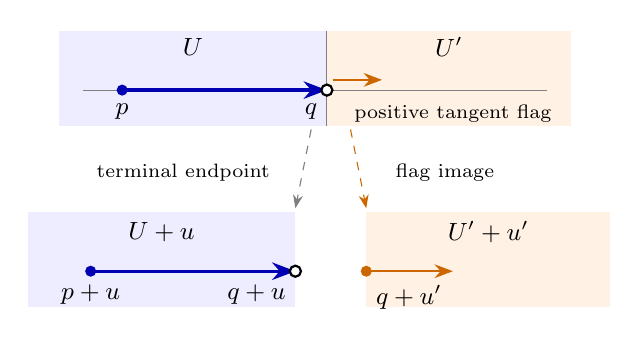
\begin{tikzpicture}[x=1cm,y=1cm,>=Stealth,font=\small]
 \fill[blue!7] (0,2.0) rectangle (3.4,3.2);
 \fill[orange!10] (3.4,2.0) rectangle (6.5,3.2);
 \draw[gray] (3.4,2.0)--(3.4,3.2);
 \node at (1.7,3.0) {$U$};
 \node at (4.95,3.0) {$U'$};
 \draw[gray] (0.3,2.45)--(6.2,2.45);
 \draw[very thick,blue!70!black,->] (0.8,2.45)--(3.4,2.45);
 \fill[blue!70!black] (0.8,2.45) circle (2pt);
 \draw[fill=white,thick] (3.4,2.45) circle (2pt);
 \draw[orange!80!black,->,thick] (3.48,2.58)--(4.1,2.58);
 \node[below] at (0.8,2.4) {$p$};
 \node[below left] at (3.4,2.4) {$q$};
 \node[below,font=\scriptsize] at (5.0,2.38) {positive tangent flag};
 \fill[blue!7] (-0.4,-0.3) rectangle (3.0,0.9);
 \fill[orange!10] (3.9,-0.3) rectangle (7.0,0.9);
 \node at (1.3,0.65) {$U+u$};
 \node at (5.45,0.65) {$U'+u'$};
 \draw[very thick,blue!70!black,->] (0.4,0.15)--(3.0,0.15);
 \fill[blue!70!black] (0.4,0.15) circle (2pt);
 \draw[fill=white,thick] (3.0,0.15) circle (2pt);
 \fill[orange!80!black] (3.9,0.15) circle (2pt);
 \draw[orange!80!black,->,thick] (3.9,0.15)--(5.0,0.15);
 \node[below] at (0.4,0.1) {$p+u$};
 \node[below left] at (3.0,0.1) {$q+u$};
 \node[below right] at (3.9,0.1) {$q+u'$};
 \draw[->,dashed,gray] (3.2,1.95)--(3.0,0.95);
 \draw[->,dashed,orange!80!black] (3.7,1.95)--(3.9,0.95);
 \node[font=\scriptsize,anchor=east] at (2.8,1.4) {terminal endpoint};
 \node[font=\scriptsize,anchor=west] at (4.15,1.4) {flag image};
\end{tikzpicture}
\caption{Endpoint transport across a chart edge.  The interval starting at
$p$ uses the activation bit transported to $p+u$.  Its terminal endpoint
$q+u$ is forced by the destination core.  The positive flag based at $q$
uses the next chart translation $u'$; its image $q+u'$ need not coincide
with $q+u$.}
\label{fig:am-endpoints}
\end{figure}

At a vertex where several chart edges meet, an interval entering an open
chart still has its positive tangent flag in that chart.  If an interval
runs along a chart boundary, that boundary is already a full barrier and
requires no activation comparison.  Parallel lines either do not cross an
edge or coincide with its supporting line; these alternatives have just
been covered.  Intersections that only touch at a point make no difference
to Boolean cells.

It remains to handle the finite line cutoff.  If $L$ is a candidate but
$L+u$ is not, then
\[
 |\bar c|\ge4N-Q>3N
\]
for sufficiently large $N$.  Every second bit at a start on $L$ is zero
by~\eqref{eq:am-negative-band}, so the line contributes no active segment.
The reverse mismatch is handled by the same inequality on the destination
line.  A line absent because it misses the square cannot produce a
mismatch inside $U,V$, since a line meeting one of these corresponding
open charts translates to a line meeting the other.  Square seam
translations were included in the bound $Q$ and in the endpoint core.
Thus active barriers inside $U$ translate exactly to the active barriers
inside $V$ in every case.

Since all chart edges are full barriers in both samples, this equality
inside each pair of open charts identifies their connected complementary
components.  Each source cell therefore translates to precisely one
destination cell, and all destination cells occur.  It follows that
$\mathcal P'=g\mathcal P$.  Finally choose $\eta,\kappa$ small enough
and then $N$ large enough that
$\varepsilon_N+2\alpha_N<\delta$, simultaneously for the finite set
$\mathcal K$.
\end{proof}

The field construction and the endpoint argument have now produced a
partition law with the required covariance.  The remaining step is a
group-theoretic conversion.  It uses uniform matchings of equal shapes to
retain covariance, followed by an explicit passage from probability
measures to the finite sets in the definition of amenability.

\subsection{Shape matchings, subgroup measures, and finite F\o lner sets}

Two nonempty polygonal cells have the same \emph{shape} if one is a
translate of the other by an element of $\OO^2$ in ordinary square
coordinates; their tracks may differ.  The translation is unique.  Indeed,
a bounded set of positive area cannot be invariant modulo empty interior
under a nonzero translation: a linear functional increasing in that
direction has a finite essential supremum, which the translation would
increase.  A finite partition has a finite multiset of shapes, counting
multiplicities.

For every multiset of shapes that occurs for a partition of $mX$, fix one
baseline partition with that multiset.  There are only countably many
partitions, so these choices require no measurability qualification.
Given a sampled partition $\mathcal P$, choose uniformly a shape-preserving
bijection from its baseline partition onto $\mathcal P$.  On each baseline
cell use the unique translating identification to the assigned cell.
Their union is a piecewise translation $a\in F_m$.  Denote its probability
law by $\nu$.

In the successful coupling of Lemma~\ref{lem:am-partition-coupling}, the
partitions $\mathcal P$ and $g\mathcal P$ have the same multiset of
shapes, because each cell lies in one translation chart.  They consequently
have the same baseline.  Composition by $g$ bijects the shape-preserving
matchings to $\mathcal P$ with the shape-preserving matchings to
$g\mathcal P$.  Thus a uniform matching to the first, followed by $g$, is
a uniform matching to the second.  Extend this coupling by arbitrary
uniform matchings on the exceptional event.  Each marginal is still the
law prescribed above, and the resulting group elements are related by
left multiplication by $g$ on the successful event.  Hence
\begin{equation}\label{eq:am-reiter}
 \|g\nu-\nu\|_{\TV}<\delta
 \qquad(g\in\mathcal K).
\end{equation}
Here $(g\nu)(a)=\nu(g^{-1}a)$, and for measures on a countable set
$\|\sigma-\sigma'\|_{\TV}=\frac12\sum_a|\sigma(a)-\sigma'(a)|$.
For the concrete construction at a fixed scale $N$ there are in fact only
finitely many possible successful marked configurations and hence finitely
many partitions and matchings.  The following argument allows countable
support as well and proves subgroup inheritance at the same time.

\begin{lemma}\label{lem:am-reiter-folner}
Let $H$ be a subgroup of a countable group $J$.  Suppose that for every
finite $K\subset H$ and every $\varepsilon>0$ there is a probability
measure $\nu$ on $J$ such that
\[
 \sum_{k\in K}\|k\nu-\nu\|_1<\varepsilon.
\]
Then for every finite $K\subset H$ and every $\varepsilon>0$ there is a
nonempty finite $A\subset H$ such that
\[
 \sum_{k\in K}|kA\mathbin\triangle A|<\varepsilon|A|.
\]
\end{lemma}

\begin{proof}
Choose one representative $t$ in every right coset $Ht$ of $H$ in $J$,
and write each $x\in J$ uniquely as $x=h t$.  Define $\pi(x)=h$.
Then $\pi(kx)=k\pi(x)$ for $k\in H$.  The pushforward
$p=\pi_*\nu$ is a probability measure on $H$, and summing over fibers
shows
\[
 \|kp-p\|_1\le\|k\nu-\nu\|_1.
\]
Start with the sum on the right less than $\varepsilon/2$.  If $K$ is
empty any singleton suffices, so assume $K$ is nonempty.  Choose a finite
$E\subset H$ with $p(E)>1-\varepsilon/(8|K|)$, decreasing this error
further if necessary to ensure $p(E)>0$, and put
$q=p\mathbf1_E/p(E)$.  Direct calculation gives
$\|q-p\|_1=2(1-p(E))$.  Therefore
\[
 \sum_{k\in K}\|kq-q\|_1
 \le \sum_{k\in K}\|kp-p\|_1
       +4|K|(1-p(E))<\varepsilon.
\]
For $t>0$ let $A_t=\{h\in H:q(h)>t\}$.  These sets are finite, and the
identities for real numbers $a,b\ge0$,
\[
 \int_0^\infty\mathbf1_{\{a>t\}}\,dt=a,
 \qquad
 \int_0^\infty
 |\mathbf1_{\{a>t\}}-\mathbf1_{\{b>t\}}|\,dt=|a-b|,
\]
give, after finite summation,
\[
 \int_0^\infty |A_t|\,dt=1,
 \qquad
 \int_0^\infty\sum_{k\in K}|kA_t\mathbin\triangle A_t|\,dt
 =\sum_{k\in K}\|kq-q\|_1<\varepsilon.
\]
If every nonempty $A_t$ had its summed boundary at least
$\varepsilon|A_t|$, integration would contradict these two formulas.
For some $t$ the nonempty finite set $A=A_t$ therefore satisfies the
asserted strict inequality.
\end{proof}

\begin{proof}[Proof of Theorem~\ref{thm:amenability}]
Fix a subgroup $H\le F_m$, a finite $K\subset H$, and $\varepsilon>0$.
For nonempty $K$, apply the construction with $\mathcal K=K\cup K^{-1}$
and with the total variation error in~\eqref{eq:am-reiter} less than
$\varepsilon/(4|K|)$.  It supplies a probability measure on $F_m$ whose
summed $\ell^1$ error for $K$ is less than $\varepsilon/2$.
Lemma~\ref{lem:am-reiter-folner} supplies a nonempty finite $A\subset H$
with summed boundary less than $\varepsilon|A|$, and hence
$|kA\mathbin\triangle A|<\varepsilon|A|$ for every $k\in K$.
The empty $K$ case is immediate.  Taking $H=F_m$ proves amenability of
$F_m$, and taking $H=A_m$ gives the assertion needed for the simple group.
All choices were made with $m$ fixed; no passage to infinitely many tracks
has occurred.
\end{proof}

\section{Finite generation of the multiplier}\label{sec:homology}

This section uses the arithmetic, strict-area comparison, and alternating
extension results of Lemmas~\ref{lem:arithmetic}, \ref{lem:comparison},
and~\ref{lem:extension}.  Its goal is
the following finiteness statement.  All homology groups in this Section have
integer coefficients unless another coefficient group is displayed.

\begin{theorem}\label{thm:multiplier}
There is an integer $m_{\mathrm{hom}}$ such that
$H_2(A_m;\ZZ)$ is finitely generated for every finite $m\geq m_{\mathrm{hom}}$.
\end{theorem}

The proof first establishes stability and finite generation for
$H_1(F_m)$ and $H_2(F_m)$.  Polygonal step functions enter through an explicit
resolution of a symmetric monoidal groupoid.  We then return to a fixed finite
number of tracks, prove that $F_m$ acts trivially on $H_2(A_m)$, and use the
homology spectral sequence of $A_m\triangleleft F_m$.  No presentation or
finite-generation assertion about $A_m$ is used in this Section.

This stability and group-completion strategy has precedents in the
Higman--Thompson calculation of Szymik and Wahl \cite{SzymikWahl2019}
and in Li's framework for ample groupoids and full groups
\cite{Li2025}.  Here the polygon category, its low-degree resolution,
and the return to $A_m$ on finitely many tracks are constructed below.
The external bar and group-completion results are cited at their
individual applications.

\subsection{Configurations of embedded squares}

An embedding $e:X\hookrightarrow mX$ means an injective partial piecewise
translation, defined on the entire Boolean square $X$.  Let $\mathcal E_m$ be
the semisimplicial set whose $p$-simplices are ordered tuples
$(e_0,\ldots,e_p)$ of embeddings with pairwise disjoint images.  Faces delete
entries.  Write $C_p(\mathcal E_m)$ for its integral chain group and augment
it by $C_{-1}(\mathcal E_m)=\ZZ$, sending every vertex to $1$.

\begin{lemma}\label{lem:hom-configuration-acyclic}
For each fixed integer $d\geq0$, the augmented complex
$C_*(\mathcal E_m)$ has zero homology in degrees $-1,0,\ldots,d$ when $m$ is
sufficiently large.  The required lower bound on $m$ depends only on $d$.
\end{lemma}

\begin{proof}
Any $b$ vertices have a common disjoint vertex if $m>b+1$: the union of their
images has area at most $b$, so its complement has area greater than $1$;
Lemma~\ref{lem:comparison} embeds $X$ in that complement.

We construct a chain contraction in the asserted degrees.  Choose a vertex
$v$ and put $h_{-1}(1)=v$.  Suppose $h_{-1},\ldots,h_{p-1}$ have been
constructed, satisfy $\partial h+h\partial=\id$ in degrees below $p$, and
the vertices appearing in $h_{p-1}(\rho)$ are bounded in number independently
of the $(p-1)$-simplex $\rho$.  For a $p$-simplex $\sigma$, the chain
\[
 z_\sigma=\sigma-h_{p-1}(\partial\sigma)
\]
is a cycle.  Its vertices have a bound depending only on $p$: if the bound
for $h_{p-1}$ is $b_{p-1}$, a valid bound is
$(p+1)+(p+1)b_{p-1}$.  Choose a vertex $w_\sigma$ disjoint from all these
vertices and define $h_p(\sigma)=w_\sigma*z_\sigma$, where the cone prepends
$w_\sigma$ to each ordered simplex.  The identity
\[
 \partial(w_\sigma*z)=z-w_\sigma*(\partial z)
\]
gives $\partial h_p(\sigma)+h_{p-1}(\partial\sigma)=\sigma$.
Moreover, $b_p=1+(p+1)+(p+1)b_{p-1}$ is a uniform bound for the vertices
appearing in $h_p(\sigma)$.  Starting with $b_{-1}=1$, choose $m$ larger
than all the finitely many bounds needed for $p\leq d$.  Linear extension
defines the required contraction.  There is no requirement that the
contraction be equivariant or that one vertex avoid an arbitrarily long
cycle.
\end{proof}

The group $F_m$ acts on $\mathcal E_m$ by postcomposition.  For a fixed $p$
and sufficiently large $m$, this action is transitive, even under $A_m$.
Indeed, the bijection from the first $p+1$ standard tracks to any given
configuration has area $p+1$ and extends by Lemma~\ref{lem:extension} when
$m>10(p+1)$.  The stabilizer in $F_m$ of the standard configuration fixes
those tracks pointwise and is therefore exactly $F_{m-p-1}$.  This avoids
any assertion that arbitrary equal-area polygons are equidecomposable.

\begin{lemma}\label{lem:hom-full-stability}
For $q=0,1,2$, adding an identity track induces an isomorphism
\[
 H_q(F_{m-1})\longrightarrow H_q(F_m)
\]
for all sufficiently large $m$.
The same assertion holds with $F_m$ replaced by the finite symmetric
group $\Sym(m)$.
\end{lemma}

\begin{proof}
Tensor the augmented configuration complex with a free right
$\ZZ[F_m]$-resolution of $\ZZ$ and take its total complex.  One filtration,
together with Lemma~\ref{lem:hom-configuration-acyclic}, shows that its
homology vanishes in any prescribed bounded range when $m$ is large.
The other filtration has, in columns $p\geq-1$,
\begin{equation}\label{eq:hom-configuration-ss}
 E^1_{p,q}=H_q(F_{m-p-1}),\qquad
 E^1_{-1,q}=H_q(F_m).
\end{equation}
Here and below only boundedly many columns are needed.  The identification
follows directly from the permutation module on simplices: restricting the
free resolution to a stabilizer is still a free resolution.

Every face inclusion of a standard stabilizer is a stabilization followed
by conjugation in the target stabilizer.  Inner conjugation induces the
identity on homology.  Thus $d^1$ is stabilization when $p$ is even and is
zero when $p$ is odd.  In particular, in row $q$ the entries at columns
$-1$ and $0$ of $E^2$ are respectively the cokernel and the kernel of
$H_q(F_{m-1})\to H_q(F_m)$.

The row $q=0$ is the alternating augmented row of copies of $\ZZ$ and is
exact.  For $q=1$, the only possible higher differentials into columns
$-1$ and $0$ come from row zero, so both entries vanish, as the total
homology vanishes.  This proves stability in degree one.  For $q=2$, the
possible sources for the entry $(-1,2)$ are $(1,1)$ and $(2,0)$, and those
for $(0,2)$ are $(2,1)$ and $(3,0)$.  The degree-one stability just proved
kills the indicated row-one entries when $m$ is increased by a fixed
amount; row zero is exact.  No higher differential has a nonnegative
source row, and there are no outgoing higher differentials from columns
$-1$ or $0$.  Hence the kernel and cokernel in degree two are zero.
Transitivity through column four and augmented acyclicity through degree
two suffice for this argument; all the requirements are finite.

For $\Sym(m)$ use ordered configurations of distinct points.  The same
bounded contraction works by choosing an unused point, the action is
transitive, and its stabilizer is $\Sym(m-p-1)$.  The identical spectral
sequence argument applies.
\end{proof}

\subsection{Group completion and three bars}

We now seek finite generation of the two stable homology groups in
Lemma~\ref{lem:hom-full-stability}.  Define $\mathcal B$ to be the
groupoid whose objects are finite lists $(U_1,\ldots,U_k)$ of Boolean
polygonal subsets of $X$.  A morphism is a piecewise translation bijection
between their disjoint unions, with the list entries serving as separate
tracks.  Tensor product is concatenation of lists; its symmetry reorders
the tracks.  The empty list is the unit.  Thus $\mathcal B$ is a strict
symmetric monoidal groupoid.  Let $\mathcal S$ be the groupoid of finite
sets and bijections, using its ordered skeleton with objects
$\{1,\ldots,n\}$, $n\geq0$.  Ordered disjoint union, with the second
block relabeled, makes its tensor product strictly associative and unital.

The groupoid $\mathcal S$ records the finite sets of track labels
over points of $X$.  By following these labels through strings of
exchanges, we will resolve $\mathcal B$ into levels built from finite
products of $\mathcal S$.  To compute their homology, we use three
bar constructions.  Reduced homology then starts in degree three,
so a product of two positive-degree classes first appears in degree
six.  The calculation through degree five is consequently additive
in the fibers; it is this range that will give stable homology
through degree two.

Here is a concrete bar convention, needed later for the resolution.
For a symmetric monoidal groupoid $\mathcal C$ and $p\geq0$, let
$D_p\mathcal C$ have objects
\[
 (C_{ij},\alpha_{ijk})_{0\leq i\leq j\leq k\leq p},\qquad
 \alpha_{ijk}:C_{ij}\sqcup C_{jk}\xrightarrow{\ \cong\ } C_{ik},
\]
with $C_{ii}$ the unit, the evident unit maps, and the associativity
condition at every four ordered indices.  Morphisms are families of
isomorphisms commuting with every $\alpha_{ijk}$.  Pullback along monotone
maps of index sets defines faces and degeneracies.  Tensor product is
coordinatewise, using the symmetry to interchange the middle summands in
the decomposition maps.  Evaluation on the elementary intervals gives an
equivalence
\begin{equation}\label{eq:hom-bar-product}
 D_p\mathcal C\simeq\mathcal C^p.
\end{equation}
An inverse replaces every interval by the ordered sum of its elementary
entries; coherence of the $\alpha$'s supplies its comparison isomorphism.

Write $B^0\mathcal C=|N\mathcal C|$ and let $B^d\mathcal C$ be the
realization of the nerve of
$D_{p_1}\cdots D_{p_d}\mathcal C$ over all $d$ bar indices.  We use
the usual realizations of these simplicial sets, or equivalently their
fat realizations.  Degeneracies are inclusions of simplicial subsets, so
these models are well based and levelwise equivalences remain
equivalences on realization.  For $M=|N\mathcal C|$, the first bar is
the usual $BM$: inserting ordered sums gives the level equivalences
with the ordinary simplicial bar.  The interval convention preserves
the symmetric product during iteration.

The coordinatewise tensor product and its symmetry make
$B^1\mathcal C$ a connected homotopy-commutative $H$-space.
We will use two standard bar facts, with their hypotheses visible in
this model.  The product equivalences
\eqref{eq:hom-bar-product}, the contractible level zero, and the
cofibration condition just noted satisfy the realization hypotheses in
\cite[Proposition~1.5 and its preceding Note; Proposition~A.1 and
Definition~A.4]{Segal1974}.
They imply that
\begin{equation}\label{eq:hom-deloop}
 B^{d-1}\mathcal C\simeq\Omega B^d\mathcal C\qquad(d\geq2).
\end{equation}
At these stages the preceding space is connected, so its component
monoid is already a group, as required by the delooping criterion.
The skeletal bar filtration also shows that
\begin{equation}\label{eq:hom-connectivity}
 \widetilde H_i(B^d\mathcal C)=0\quad(i<d),
 \qquad \pi_1(B^d\mathcal C)=0\quad(d\geq2).
\end{equation}
For example, after the first bar the spaces are connected.  In the next
bar the normalized level-zero row contributes only the base point, and
the first possible positive homology in the other levels gains one in
total degree.  The same product model, or the fundamental-group
calculation of the bar, gives simple connectivity from the second bar
onward.  This proves the displayed homological range inductively.

For $\mathcal C=\mathcal B$, our immediate target is therefore
finite generation of $H_i(B^3\mathcal B)$ for $i\leq5$.
Delooping will lower this bound to degree four for $B^2\mathcal B$
and then to degree three for $B^1\mathcal B$.  The spaces
$B^3\mathcal B$ and $B^2\mathcal B$ are simply connected, whereas
$B^1\mathcal B$ may have a nontrivial
fundamental group.  Its connected $H$-space structure will allow us
to pass to its universal cover without losing finite generation;
looping that cover gives the component $\Omega_0B^1\mathcal B$
of the constant loop, now through degree two.  Group completion
will identify this last homology with the stable homology of $F_m$.
The following lemma supplies the finiteness implications in this
chain.

\begin{lemma}\label{lem:hom-finiteness-transfers}
The following statements hold for spaces of CW homotopy type.
\begin{enumerate}[label=(\roman*)]
\item If $Z$ is simply connected, then, for every $r\geq0$,
$H_i(Z)$ is finitely generated for $i\leq r+1$ if and only if
$H_i(\Omega Z)$ is finitely generated for $i\leq r$.
\item Let $Y$ be a connected $H$-space.  If $H_i(Y)$ is finitely
generated for $i\leq r$, then $\pi_1(Y)$ and
$H_i(\widetilde Y)$ for $i\leq r$ are finitely generated, provided
$r\geq1$.  Conversely, if $\pi_1(Y)$ and those cover homology groups
are finitely generated, then $H_i(Y)$ is finitely generated for
$i\leq r$.
\end{enumerate}
\end{lemma}

\begin{proof}
We use the Serre homology spectral sequence in the form of
\cite[Theorem~1.3, p.~8]{HatcherSpectralSequences}.
For (i), apply it to the path-loop fibration, obtaining
\[
 E^2_{a,b}=H_a(Z;H_b(\Omega Z))\Longrightarrow H_{a+b}(PZ),
 \qquad PZ\simeq *.
\]
All coefficients are constant because $Z$ is simply connected.
If the base homology is finitely generated through degree $r+1$,
induct on $b\leq r$.  The term $E^2_{0,b}=H_b(\Omega Z)$ has no
outgoing differential.  Its incoming sources have strictly smaller
fiber degree and base degree at most $b+1$.  They are finitely
generated by induction and the universal coefficient theorem.  The
term at infinity is zero for $b>0$, so finitely many finitely
generated images exhaust $H_b(\Omega Z)$.  For the converse, induct
on $a\leq r+1$ in the row-zero term $E^2_{a,0}=H_a(Z)$.  It has no
incoming differential, its outgoing targets have smaller base
degree and fiber degree at most $a-1$, and its limiting term is
zero for $a>0$.  The successive quotients in this finite filtration
are subgroups of finitely generated groups.  This proves (i).

For (ii), the two products on based loops, concatenation and the
$H$-space product, give the same operation on $\pi_1(Y)$ and make
it abelian.  Thus $\pi_1(Y)=H_1(Y)$.  This fundamental group acts
trivially on the homology of the universal cover.  To see the latter
claim, represent a deck transformation by a loop $\alpha$ at the
unit.  Lift the family of maps
$(t,y)\mapsto\alpha(t)y$ to the universal cover, starting with the
identity (using the unit homotopy if necessary).  Its terminal map
is the deck transformation represented by $\alpha$.  Consequently
that map is homotopic to the identity.

Put $Q=\pi_1(Y)$.  The spectral sequence for the universal cover is
\[
 E^2_{a,b}=H_a(Q;H_b(\widetilde Y))\Longrightarrow H_{a+b}(Y),
\]
with constant coefficients.  A finitely generated abelian group
has finitely generated homology in each degree with finitely
generated constant coefficients: tensor the resolutions for an
infinite cyclic group and for a finite cyclic group.  Induction on
$b$ in column zero now proves the forward implication, since all
incoming sources have lower fiber degree and the limiting term is
a subgroup of $H_b(Y)$.  The reverse implication follows directly
from the finitely many terms on each total-degree diagonal.
\end{proof}

\begin{lemma}\label{lem:hom-cofinal-completion}
There are natural homology isomorphisms
\begin{align*}
 \underset{m}{\operatorname{colim}}\,H_j(F_m)
   &\cong H_j(\Omega_0 B^1\mathcal B),\\
 \underset{m}{\operatorname{colim}}\,H_j(\Sym(m))
   &\cong H_j(\Omega_0 B^1\mathcal S).
\end{align*}
Here $\Omega_0$ denotes the component of the constant loop.
\end{lemma}

\begin{proof}
The monoid $M=|N\mathcal B|$ is well based and has CW homotopy type.
The symmetry supplies a homotopy between the two orders of
multiplication, so $\pi_0(M)$ is central in the integral Pontryagin
ring.  The integral group-completion theorem
\cite[Proposition~1]{McDuffSegal1976} therefore identifies the
homology of $\Omega BM$ with the localization of $H_*(M)$ at its
components.

There is one cofinal object here.  The object
$U=(U_1,\ldots,U_k)$ has complement
$U^c=(X\setminus U_1,\ldots,X\setminus U_k)$ and
$U\sqcup U^c\cong kX$.  Hence inverting $X$ inverts every
component.  Its localization is computed by the telescope
\[
 T=\operatorname{tel}(M\xrightarrow{X\sqcup-}M
                  \xrightarrow{X\sqcup-}\cdots).
\]
Equivalently, every right translation on this telescope is a
homology equivalence: translation by $X$ is invertible, tensor
symmetry exchanges left and right translations, and a complement
gives an inverse for translation by any object.  This verifies the
action hypothesis in the telescope form of group completion \cite[Proposition~2 and p.~281]{McDuffSegal1976};
see also the corrected proof in
\cite[Theorem~4.1]{MillerPalmer2015}, applied with ordinary integral
homology.  In the nerve-realization model, $M$ is a Hausdorff,
locally contractible CW complex and its telescope is Hausdorff,
as required there.

The bar two-skeleton identifies $\pi_1(BM)$ with the group
completion of the commutative monoid of object-isomorphism classes:
an object supplies a loop, and a pair supplies the relation that
its sum represents the product.  The component of an object $U$
at stage $r$ of $T$ is therefore $[U]-r[X]$.  If this is zero,
there is an object $V$ with
$U\sqcup V\cong rX\sqcup V$.  Choose $V'$ with
$V\sqcup V'\cong kX$.  Then
\[
 U\sqcup kX\cong(r+k)X.
\]
Thus every component occurring in the neutral telescope component
eventually becomes a standard component $BF_{r+k}$.  Choices of
the identifying isomorphism differ by an inner automorphism and
give the same map on homology.  It follows that the neutral
component has homology $\operatorname{colim}_m H_j(F_m)$, with
the usual stabilization maps.  Group completion respects these
component gradings, proving the first assertion.  For
$\mathcal S$, use a singleton in place of $X$; the same argument
gives the second assertion.
\end{proof}

\begin{lemma}\label{lem:hom-finite-set-bars}
For $d=1,2,3$, the groups $H_i(B^d\mathcal S)$ are finitely
generated for $i\leq d+2$.
\end{lemma}

\begin{proof}
Finite groups have finitely generated integral homology in every
degree, as their bar chain groups have finite rank in each degree.
Lemma~\ref{lem:hom-full-stability} therefore gives finite
generation of the stable homology of $\Sym(m)$ through degree two.
By Lemma~\ref{lem:hom-cofinal-completion}, this is the homology
through degree two of $\Omega_0 B^1\mathcal S$, or equivalently
of $\Omega\widetilde{B^1\mathcal S}$.
Lemma~\ref{lem:hom-finiteness-transfers}(i) gives finite
generation for the cover through degree three.  The fundamental
group of $B^1\mathcal S$ is the group completion of $\NN$, hence
$\ZZ$.  Part (ii) gives finite generation for $B^1\mathcal S$
through degree three.

Ascend the bars using their skeletal filtrations and the product
models \eqref{eq:hom-bar-product}.  In the normalized filtration
for the next bar, column zero is a point, so a positive-degree
term of total degree at most $d+2$ has bar degree at least one
and internal degree at most $d+1$.  The induction hypothesis and
the integral K\"unneth theorem make the homology of every finite
product in this range finitely generated.  There are finitely
many bidegrees on each relevant diagonal.  This proves the
assertion successively for $d=2$ and $d=3$.
\end{proof}

Consequently the three coefficient groups
\begin{equation}\label{eq:hom-Kj}
 K_j=H_j(B^3\mathcal S),\qquad j=3,4,5,
\end{equation}
are finitely generated.  The remaining task is to obtain the same
degree-five bound for $B^3\mathcal B$.  We first describe its
resolution completely, including the maps that identify it.

\subsection{Strings and the trajectory differential}

We now construct the resolution whose levels have finite-set fibers.
A string of exchanges records both the positions visited by a point
and the track labels carried along that path.  Keeping these two
kinds of data separate will turn its low-degree homology into a
translation-homology calculation.

A position-preserving isomorphism of objects of $\mathcal B$ may
change the track label, piecewise, but leaves the point of $X$
unchanged.  Denote the subgroupoid of such isomorphisms, with all
objects retained, by $\mathcal P$.  For $p\geq0$ define
$\mathcal C_p$ as follows.  Its objects are strings
\[
 U_0\xrightarrow{f_1}U_1\xrightarrow{f_2}\cdots
       \xrightarrow{f_p}U_p
\]
of arbitrary morphisms of $\mathcal B$.  Its morphisms are
commuting ladders whose maps $U_i\to U'_i$ belong to
$\mathcal P$.  Deleting a vertex and composing adjacent arrows
defines the faces; inserting an identity defines the degeneracies.
Concatenation gives a simplicial symmetric monoidal groupoid.
A simplex of $N_q\mathcal C_p$ is a commuting grid with $p$
horizontal arrows and $q$ vertical arrows: the horizontal arrows
are arbitrary exchanges, and the vertical arrows preserve positions.

We first describe these strings by their trajectories and finite fibers.
For $x\in X$ and $\gamma_1,\ldots,\gamma_p\in\Gamma$, a
trajectory is the sequence of positions
\[
 x,\quad x+\gamma_1,\quad x+\gamma_1+\gamma_2,\quad\ldots,
 \quad x+\gamma_1+\cdots+\gamma_p.
\]
Cut a string in $\mathcal C_p$ according to its successive
translation charts and the inverse images of later cuts.  Each
resulting strand has a fixed increment tuple
$(\gamma_1,\ldots,\gamma_p)$ and a Boolean set of initial points.
The translation action on $X$ is free, so the increments are
uniquely determined by the positions.  Track multiplicities give
a finite set over each initial point and increment tuple.
Position-preserving ladders are exactly permutations of these
fibers.  Conversely, a Boolean locally constant family of finite
sets on $X\times\Gamma^p$, supported on finitely many increment
tuples, reconstructs a string by taking its strands as separate
list entries and translating them successively.  These
constructions give an equivalence of symmetric monoidal
groupoids.

More explicitly, restrict to a finite set of increment tuples
and a finite Boolean partition on which all fiber sets and maps
are constant.  The corresponding groupoid is a finite product
of copies of $\mathcal S$.  Enlarging the finite support inserts
empty fibers; refining an atom duplicates its fiber.  Every
finite diagram of strings and isomorphisms occurs at one such
stage.  Thus nerves, bars, and their chain complexes are obtained
by a filtered colimit of these finite stages.

The levels are now expressed in terms of finite sets.  The next lemma
shows that realizing the spaces $B^3\mathcal C_p$ in the string index
$p$ recovers $B^3\mathcal B$.  The commuting-grid description is the
basis of its proof.

\begin{lemma}\label{lem:hom-string-resolution}
There is a zigzag of natural realization equivalences between
$B^3\mathcal B$ and the realization in $p$ of $B^3\mathcal C_p$.
\end{lemma}

\begin{proof}
Fix three bar indices $\boldsymbol n=(n_1,n_2,n_3)$, and put
$\mathcal D=D_{n_1}D_{n_2}D_{n_3}\mathcal B$.
Let $\mathcal D^{\mathrm{pos}}$ have those objects of
$\mathcal D$ whose decomposition isomorphisms at every bar level
preserve positions in $X$, but retain \emph{all} horizontal diagram isomorphisms
between them.  The inclusion
\begin{equation}\label{eq:hom-pos-inclusion}
 \mathcal D^{\mathrm{pos}}\longrightarrow\mathcal D
\end{equation}
is full and essentially surjective.  Indeed, replace every
multi-interval object by the lexicographically ordered sum of its
elementary entries, indexed by products of consecutive intervals
$[i_1-1,i_1]\times[i_2-1,i_2]\times[i_3-1,i_3]$ in the three
bar-index sets.  Its decomposition maps are
canonical reorderings and preserve positions.  The original
coherent decomposition maps identify each ordered sum with the
corresponding original multi-interval.  They form a diagram
isomorphism because changing the order of the cuts only introduces
the specified symmetric reordering.  The comparison is allowed to
translate pieces: it is a horizontal arrow.  For example, in one
bar at degree two, the long edge $U_{02}$ is replaced by
$U_{01}\sqcup U_{12}$, and the comparison on that edge is the
original map $\alpha_{012}$, regardless of whether it preserves
positions.

The inclusions \eqref{eq:hom-pos-inclusion} commute with all bar
operations.  A face pulls back the existing interval diagram and its
specified decomposition maps; it does not choose a new ordered-sum
normalization.  Composing position-preserving decompositions,
inserting a unit, and reordering sums remain position-preserving.
We use these inclusions as the natural maps; no strictly natural
choice of an inverse normalization is required.

Now take the double nerve whose horizontal strings use arbitrary
arrows of $\mathcal D^{\mathrm{pos}}$ and whose vertical arrows
preserve positions.  Reading it horizontally first gives exactly
the nerve of $D_{n_1}D_{n_2}D_{n_3}\mathcal C_p$: its
decomposition maps are position-preserving ladders, precisely the
condition built into the morphisms of $\mathcal C_p$.

Read the same double nerve vertically first, fixing a vertical
string length $q$.  Its groupoid has objects strings
$V_0\xrightarrow{v_1}\cdots\xrightarrow{v_q}V_q$ of
position-preserving arrows and has arbitrary horizontal commuting
ladders.  Evaluation at $V_0$ is an equivalence with
$\mathcal D^{\mathrm{pos}}$.  It is essentially surjective by
constant strings.  It is fully faithful because a horizontal
arrow $a_0:V_0\to W_0$ uniquely determines all its components:
\begin{equation}\label{eq:hom-ladder-formula}
 a_i=w_{0i}\,a_0\,v_{0i}^{-1},
 \qquad v_{0i}=v_i\cdots v_1,
 \quad w_{0i}=w_i\cdots w_1.
\end{equation}
Every map in \eqref{eq:hom-ladder-formula} is an allowed
horizontal diagram map.  Constant-string inclusions are natural
in $q$ and in every bar index, and are levelwise equivalences.
Thus the constant-string maps and
\eqref{eq:hom-pos-inclusion} give the asserted zigzag after taking
nerves and successive realizations.  The levelwise-equivalence
criterion applies to these simplicial-set models as explained
before \eqref{eq:hom-deloop}.
\end{proof}

We now apply this finite-fiber description to homology.
Put $E=B^3\mathcal S$.  By \eqref{eq:hom-connectivity},
$H_0(E)=\ZZ$ and $\widetilde H_i(E)=0$ for $i<3$.
For a finite product $E^s$, the integral K\"unneth formula gives
\begin{equation}\label{eq:hom-product-additivity}
 H_j(E^s)=\bigoplus_{a=1}^s H_j(E)
 \qquad(j=3,4,5).
\end{equation}
A tensor term using two positive-degree factors first has degree
six; a corresponding $\operatorname{Tor}$ term first has degree
seven.  Terms involving $H_0(E)=\ZZ$ have no such torsion term.
The disjoint-union map on the fibers restricts to the identity
on either factor when the other is empty.  Hence under
\eqref{eq:hom-product-additivity} it induces ordinary addition.
Refinement induces the diagonal, since the same fiber is copied
onto every new atom.  Exactness of filtered colimits therefore
identifies
\begin{equation}\label{eq:hom-trajectory-chains}
 H_j(B^3\mathcal C_p)
  =\bigoplus_{(\gamma_1,\ldots,\gamma_p)\in\Gamma^p}
        C(X,\ZZ)\otimes K_j\qquad(j=3,4,5),
\end{equation}
where $C(X,\ZZ)$ denotes the Boolean step functions.  There is
no derived tensor hidden here: $C(X,\ZZ)$ is the filtered union
of the free groups of functions on finite Boolean partitions.

For clarity, all the differential maps in
\eqref{eq:hom-trajectory-chains} can be written on trajectories:
\begin{align}
 d_0(x;\gamma_1,\ldots,\gamma_p)
   &=(x+\gamma_1;\gamma_2,\ldots,\gamma_p),\notag\\
 d_i(x;\gamma_1,\ldots,\gamma_p)
   &=(x;\gamma_1,\ldots,\gamma_i+\gamma_{i+1},\ldots,\gamma_p),
       &&0<i<p,\label{eq:hom-trajectory-faces}\\
 d_p(x;\gamma_1,\ldots,\gamma_p)
   &=(x;\gamma_1,\ldots,\gamma_{p-1}).\notag
\end{align}
Fibers acquiring the same label are disjointly summed.  In the
coefficient convention $\gamma_*f(y)=f(y-\gamma)$, the first face
therefore applies $\gamma_{1*}$ to the coefficient, each interior
face adds two consecutive increments, and the last face leaves
the coefficient unchanged.  The alternating sum of these maps is
the inhomogeneous group-homology bar differential for the
translation module $C(X,\ZZ)\otimes K_j$ (the group $\Gamma$ is
abelian, so the same pushforward convention also gives a right
module).

The skeletal spectral sequence for the resolution in
Lemma~\ref{lem:hom-string-resolution} consequently has, in the
reduced rows relevant to total degree at most five,
\begin{equation}\label{eq:hom-trajectory-ss}
 E^2_{p,j}
   =H_p\bigl(\Gamma;C(X,\ZZ)\otimes K_j\bigr),
       \qquad j=3,4,5.
\end{equation}
Rows one and two are zero.  Row zero is the constant simplicial
group $\ZZ$, since every $B^3\mathcal C_p$ is connected; its
homology contributes only the degree-zero copy of $\ZZ$.
We now establish finite generation of the coefficient homology
in \eqref{eq:hom-trajectory-ss}.

\subsection{Corner symbols and polygonal coefficients}

Let $H=\OO^2$, regarded as a discrete free abelian group of rank
four, and let $L$ be the abelian group of compactly supported
integer-valued step functions on the plane whose boundaries use
finitely many allowable lines.  Equalities are modulo sets with
empty interior.  Translations make $L$ a module over
\[
 R=\ZZ[H]\cong
       \ZZ[t_1^{\pm1},t_2^{\pm1},t_3^{\pm1},t_4^{\pm1}],
\]
a noetherian ring.

Translation modules of polyhedral step functions also occur in the
homology of projection-method patterns
\cite[Section~3.1]{GahlerHuntonKellendonk2013}.  Our immediate task is
the integral finite-generation statement below.  We prove it by an
explicit corner map and the finite vertex types of
Lemma~\ref{lem:arithmetic}, without a cut-and-project identification.

\begin{lemma}\label{lem:hom-corner-module}
The $R$-module $L$ is finitely generated.
\end{lemma}

\begin{proof}
Let $V$ be the set of intersections of at least two nonparallel
allowable lines.  At $z\in V$, let $r(z)\in\{2,3,4\}$ be the
number of allowable lines through $z$.  Their $2r(z)$ sectors
give a free abelian group of sector germs.  Quotient it by the
constant germ and the indicator germs of either half-plane for
each incident line; call the quotient $Q_z$.

We spell out this integral quotient.  Number the sectors
cyclically, put $r=r(z)$, and write a germ as
$(a_0,\ldots,a_{2r-1})$.  With indices modulo $2r$, let
\[
 d_i=a_{i+1}-a_i,\qquad q_i=d_i+d_{i+r}\quad(0\leq i<r).
\]
Then $\sum_iq_i=0$, and
\begin{equation}\label{eq:hom-corner-quotient}
 Q_z\cong\{(q_0,\ldots,q_{r-1})\in\ZZ^r:\textstyle\sum_iq_i=0\}
       \cong\ZZ^{r-1}.
\end{equation}
Indeed, cyclic differences identify germs modulo constants with
$\{d\in\ZZ^{2r}:\sum_i d_i=0\}$.  A half-plane germ has
difference vector $\pm(e_i-e_{i+r})$.  These vectors generate
exactly the kernel of the pair-sum map $d\mapsto q$; the map is
onto, since $d=(q,0)$ has zero total sum.  This proves
\eqref{eq:hom-corner-quotient} over $\ZZ$.

For $f\in L$, record its sector germ modulo this subgroup at
every $z$.  The result is a translation-equivariant map
\[
 c:L\longrightarrow\bigoplus_{z\in V}Q_z.
\]
This has finite support.  To define the germ, use the finite line
family defining $f$ and take a small neighborhood excluding its
nonincident lines; other allowable directions through $z$
merely refine sectors with equal values.  A nonzero symbol can
occur only where two of the finitely many defining lines cross.
The density of the collection of all allowable lines causes no
difficulty.

The map $c$ is injective.  If $c(f)=0$, the equation
$d_{i+r}=-d_i$ says that the jump across each incident oriented
line is the same on both sides of the vertex.  Fix a line in a
finite defining family for $f$.  Its jump is constant between
successive intersections with that family and, by the preceding
identity, continues unchanged across every intersection.  It is
therefore constant along the whole line.  Compact support makes
the jump zero far away, hence everywhere.  All the line jumps
vanish.  Any two chambers of the finite line arrangement can be
joined by a path crossing its lines away from vertices; their
function values consequently agree.  The common value is zero
outside the compact support, so $f=0$.

Lemma~\ref{lem:arithmetic} places $V$ inside
$D^{-1}\OO^2$ for a fixed integer $D>0$.  Thus $V$ has finitely
many $H$-orbits; translation preserves the full set of incident
directions, and a point has trivial translation stabilizer.
After choosing one representative from each orbit,
\[
 \bigoplus_{z\in V}Q_z
       \cong\bigoplus_{\alpha=1}^s
                    R^{\,r(z_\alpha)-1}.
\]
This is a finite free $R$-module.  Its submodule $c(L)$ is
finitely generated because $R$ is noetherian, proving the Lemma.
\end{proof}

\begin{lemma}\label{lem:hom-coefficient-finiteness}
For every finitely generated abelian group $K$ and every $i\geq0$,
\[
 H_i\bigl(\Gamma;C(X,\ZZ)\otimes K\bigr)
\]
is a finitely generated abelian group.
\end{lemma}

\begin{proof}
Put $N=\ZZ^2$ and $J=\tau\ZZ^2$.  Then
$H=N\oplus J$ and $J\cong\Gamma$.  Cutting a compactly
supported function along the integer square grid gives, as
$N$-modules,
\begin{equation}\label{eq:hom-square-induction}
 L\cong\ZZ[N]\otimes C(X,\ZZ).
\end{equation}
The second factor is represented by functions supported in one
unit square, and $N$ shifts the square index.  Only finitely many
squares meet any given support.  The Boolean convention makes
the half-open choice on square edges immaterial.

Tensor \eqref{eq:hom-square-induction} with $K$.  Induction from
the trivial subgroup, or the two-generator free abelian
resolution, gives
\[
 H_q(N;L\otimes K)=
 \begin{cases}
 C(X,\ZZ)\otimes K,&q=0,\\
 0,&q>0.
 \end{cases}
\]
On the coinvariants, a translation in $J$ cuts and moves pieces
back to the chosen square, so its action is exactly translation
modulo one.  Taking the two successive free abelian resolutions
for $N$ and $J$ therefore identifies
\begin{equation}\label{eq:hom-plane-torus}
 H_i(H;L\otimes K)
   \cong H_i\bigl(\Gamma;C(X,\ZZ)\otimes K\bigr).
\end{equation}

By Lemma~\ref{lem:hom-corner-module}, $L\otimes K$ is a
finitely generated $R$-module: tensor a finite set of $R$-module
generators of $L$ with a finite set of abelian generators of $K$.
The Koszul resolution on $t_1-1,\ldots,t_4-1$ computes the
left side of \eqref{eq:hom-plane-torus}.  Its chain groups are
finite sums of $L\otimes K$, and its homology is finitely
generated over $R$ by noetherianity.  On this complex, exterior
multiplication $\varepsilon_a$ by the $a$th basis vector satisfies
\[
 d\varepsilon_a+\varepsilon_a d=(t_a-1)\id.
\]
Thus each $t_a-1$ acts trivially on homology.  The homology is
therefore a finitely generated module over
$R/(t_1-1,\ldots,t_4-1)=\ZZ$, as required.  We have proved
finite generation of $L$ integrally before tensoring; no
preservation of the corner-map injection under tensor product
is being assumed.
\end{proof}

\begin{proposition}\label{prop:hom-full-finiteness}
For all sufficiently large finite $m$, the groups $H_1(F_m)$
and $H_2(F_m)$ are finitely generated.
\end{proposition}

\begin{proof}
By Lemma~\ref{lem:hom-finite-set-bars}, each $K_j$ in
\eqref{eq:hom-Kj} is finitely generated.
Lemma~\ref{lem:hom-coefficient-finiteness} makes every relevant
term of \eqref{eq:hom-trajectory-ss} finitely generated.
There are finitely many terms of total degree at most five,
apart from the rows already shown to vanish.  Hence
Lemma~\ref{lem:hom-string-resolution} gives finite generation
of $H_i(B^3\mathcal B)$ for $i\leq5$.

Apply \eqref{eq:hom-deloop} and
Lemma~\ref{lem:hom-finiteness-transfers}(i) twice.  First
$H_i(B^2\mathcal B)$ is finitely generated for $i\leq4$, and
then $H_i(B^1\mathcal B)$ is finitely generated for $i\leq3$.
Both bases in these applications are simply connected by
\eqref{eq:hom-connectivity}.  The connected $H$-space
$B^1\mathcal B$ has finitely generated abelian fundamental
group, and part (ii) of the same Lemma gives finite generation
of its universal-cover homology through degree three.  Part (i)
now gives finite generation of
$H_i(\Omega_0 B^1\mathcal B)$ for $i\leq2$.
Lemma~\ref{lem:hom-cofinal-completion} identifies these with
the stable homology groups of $F_m$, and
Lemma~\ref{lem:hom-full-stability} transfers the conclusion to
every sufficiently large finite $m$.
\end{proof}

\subsection{Returning to the alternating group on finitely many tracks}

Only the passage from full-group homology to the multiplier
remains.  We must control the conjugation action on the whole
group $H_2(A_m)$, because a bound on its coinvariants alone would
not prove Theorem~\ref{thm:multiplier}.

\begin{lemma}\label{lem:hom-alternating-surjection}
For all sufficiently large $m$, stabilization induces a
surjection $H_2(A_{m-1})\to H_2(A_m)$.
\end{lemma}

\begin{proof}
Use the action of $A_m$ on $\mathcal E_m$.  It is transitive
in the bounded range of degrees needed here, by
Lemma~\ref{lem:extension}.  For the standard $p$-simplex, its
stabilizer is
\[
 A_m\cap F_{m-p-1}
 =\ker\bigl(F_{m-p-1}\longrightarrow F_m/A_m\bigr).
\]
By Theorem~\ref{thm:simplicity}, $A_t=[F_t,F_t]$.
The degree-one stability from
Lemma~\ref{lem:hom-full-stability} identifies
$H_1(F_{m-p-1})\to H_1(F_m)$ as an isomorphism when $m$ is
large and $p$ is bounded.  The displayed kernel is therefore
exactly $A_{m-p-1}$.

The augmented spectral sequence now has
$E^1_{p,q}=H_q(A_{m-p-1})$ and augmented column
$E^1_{-1,q}=H_q(A_m)$.  Its $E^2_{-1,2}$ is the cokernel
of the stabilization map in the statement.  Every $A_t$ is
perfect, so the row $q=1$ vanishes; row zero is the exact
alternating row of copies of $\ZZ$.  The only possible higher
incoming differentials at $(-1,2)$ have sources $(1,1)$ for
$d^2$ and $(2,0)$ for $d^3$.  They are zero on their respective
pages.  There is no outgoing differential from column $-1$.
The limiting term vanishes by
Lemma~\ref{lem:hom-configuration-acyclic}, so the cokernel
is zero.
\end{proof}

\begin{lemma}\label{lem:hom-trivial-action}
For all sufficiently large finite $m$, conjugation by every
element of $F_m$ induces the identity on $H_2(A_m)$.
\end{lemma}

\begin{proof}
Choose one finite integer $b$ such that all the stabilization
maps in Lemma~\ref{lem:hom-alternating-surjection} are
surjective once the target index exceeds $b$.  Composition gives
\[
 H_2(A_b)\twoheadrightarrow H_2(A_m)\qquad(m\geq b).
\]
Let $Y$ be the first $b$ tracks of $mX$, and take $m>10b$.
For $f\in F_m$, the restriction $f|_Y:Y\to f(Y)$ is a
piecewise translation between sets of area $b$.
Lemma~\ref{lem:extension} supplies $a\in A_m$ that agrees
with $f$ on $Y$.  For every $h\in A_b$, viewed as supported
on $Y$, one has the exact equality
\[
 f h f^{-1}=a h a^{-1}.
\]
Conjugation by $a$ is inner in $A_m$ and acts trivially on
its homology.  The two induced maps agree on the image of
$H_2(A_b)$, which is all of $H_2(A_m)$.  This proves the
claim.  The bank $Y$ is fixed independently of both $f$ and the
homology class; only the extending element $a$ depends on $f$.
\end{proof}

\begin{proof}[Proof of Theorem~\ref{thm:multiplier}]
Fix a finite $m$ beyond the thresholds in
Proposition~\ref{prop:hom-full-finiteness} and
Lemma~\ref{lem:hom-trivial-action}.  Put $Q=F_m/A_m$.
Theorem~\ref{thm:simplicity} identifies $Q$ with $H_1(F_m)$,
so $Q$ is finitely generated abelian.  Apply the integral
Lyndon--Hochschild--Serre spectral sequence
\cite[6.8.2, pp.~195--196]{Weibel1994} to
$1\to A_m\to F_m\to Q\to1$:
\[
 E^2_{p,q}=H_p(Q;H_q(A_m))\Longrightarrow H_{p+q}(F_m).
\]
By Lemma~\ref{lem:hom-trivial-action},
$E^2_{0,2}=H_2(A_m)$ itself.  Perfection gives
$H_1(A_m)=0$, so the possible incoming $d^2$ from $(2,1)$
vanishes.  The only remaining possible incoming differential is
\[
 d^3:E^3_{3,0}\longrightarrow E^3_{0,2}=H_2(A_m).
\]
Its source is a subquotient of $H_3(Q)$ and is finitely
generated.  Later incoming differentials have negative source
row, and none can leave column zero.  Consequently
\[
 E^\infty_{0,2}=H_2(A_m)/\im(d^3).
\]
This limiting term is the bottom filtration subgroup of
$H_2(F_m)$, which is finitely generated by
Proposition~\ref{prop:hom-full-finiteness}.  Both
$\im(d^3)$ and the displayed quotient are finitely generated,
so $H_2(A_m)$ is finitely generated.  All thresholds used in
choosing $m$ are fixed finite integers, and the argument applies
to every larger finite $m$.
\end{proof}

\section{Finite relations and a calculus of conditional permutations}
\label{sec:lifting}

The input to this section is the polygon Boolean algebra, its translation
action, and the identity $A_m=[F_m,F_m]$ proved in
Theorem~\ref{thm:simplicity}.  We construct a finite presentation mapping
onto $A_m$ and establish the algebraic rules used to propagate its
relations.  At this stage its kernel is not known to be central.  The
point is to identify precisely which local identities suffice for the
geometric argument in Section~\ref{sec:propagation} and the transport
argument in Section~\ref{sec:transport}.

Throughout the section an \emph{alphabet} is a subset of the $m$ track
indices.  A conditional permutation on a Boolean set $U\subseteq X$
permutes the tracks at the points of $U$ and fixes their complement.
We call $U$ a \emph{test}.  Coordinates of different tracks are aligned
unless offsets are explicitly specified.  We use
$[g,h]=ghg^{-1}h^{-1}$ and write
\[
 B_m=\{d=(d_1,\ldots,d_m)\in\Gamma^m:\textstyle\sum_i d_i=0\}.
\]
Its elements are the balanced translations.  Since
$\OO/\ZZ$ is infinite cyclic, $B_m$ is free abelian of rank $2(m-1)$.

\subsection{Generators and the finite initial choice}

Let $\alpha=\tau\bmod1$.  Choose a sufficiently small square $Q$ about
the origin in a circular coordinate chart, with side levels in $\OO$.
Our initial finite collection $\mathcal U_0$ consists of $X$, the two
coordinate interval tests with endpoints $0,\alpha$, and the two tests
\[
 Q\cap\{y-\lambda x>0\},\qquad
 Q\cap\{x-\lambda y>0\}.
\]
Boundary conventions make no difference in the Boolean algebra.
Complements are generated using the constant permutations, so they
need not be additional basic tests.

For $U\in\mathcal U_0$ and every even permutation $\sigma$ supported
on at most five tracks, include a generator $c_{U,\sigma}$.  Include
also the balanced translations
\begin{equation}\label{eq:lifting-generators}
 t_{i,r}=t(\varepsilon_r e_i-\varepsilon_r e_m),
 \qquad i<m,\quad r=1,2,
 \qquad
 \varepsilon_1=(\alpha,0),\quad\varepsilon_2=(0,\alpha).
\end{equation}
Here $e_i$ designates a track, and the notation $t(d)$ denotes the
corresponding piecewise translation.  This is a finite list, denoted
by $S_m$.  The conditional permutations belong to $A_m$.  The balanced
translations do as well: if $i,j,k,h$ are distinct, $v\in\Gamma$, and
$\sigma=(i\ j\ k)$, then in $F_m$
\begin{equation}\label{eq:translation-commutator}
 [\sigma,t(v e_i-v e_h)]=t(v e_j-v e_i).
\end{equation}
The right side is a commutator in $F_m$, and these differences generate
$B_m$.

\begin{lemma}\label{lem:lifting-generation}
For sufficiently large finite $m$, the list $S_m$ generates $A_m$.
Every polygonal test on a proper alphabet of at least five tracks
is generated, in projection to $A_m$, using conditional permutations
on translated basic tests on that alphabet and balanced translations.
\end{lemma}

\begin{proof}
First consider the Boolean algebra.  Translate the coordinate interval
test by $i\alpha$, with $i$ in an integer interval.  The endpoints of
these tests form a connected path in the orbit-index graph: each test
joins $i\alpha$ to $(i+1)\alpha$.  Two different complementary arcs
of the resulting endpoint set have different test assignments.  Indeed,
an arc between points with identical assignments contains either both
endpoints of every such edge or neither; connectedness then says it
contains all endpoints or none.  The two points therefore belong to
the same complementary arc.  Enlarging the index interval consequently
produces every circular interval whose endpoints lie in $\OO/\ZZ$.
The two coordinate families generate the rectangular Boolean algebra.

Every allowed inclined line is a translate of its line through the
origin.  The allowable tangent translations are dense along the line
by Lemma~\ref{lem:arithmetic}.  Translated copies of $Q$ therefore
cover each relevant compact segment of that line.  In each of finitely
many such charts the translated basic sign test gives its side decision;
rectangular tests clip the decision to the chart.  A finite cover of
the finitely many edges in a polygonal description proves that all
polygonal tests are Boolean combinations of translates of
$\mathcal U_0$.

Fix an alphabet $I$ with $|I|\ge5$.  The group $\Alt(I)$ is perfect.
For completeness, it is generated by $3$-cycles, and the commutator of
two $3$-cycles meeting in one letter is a $3$-cycle.  Conjugating this
identity gives all the generators.  If copies of this group on $U$
and $V$ are available in $A_m$, then
\[
 [g\text{ on }U,h\text{ on }V]=[g,h]\text{ on }U\cap V.
\]
Perfection gives every conditional permutation on $U\cap V$.
The product of the constant $g$ and the inverse of $g$ on $U$ gives
$g$ on $U^c$.  This constructs all Boolean combinations in projection.
A common translation on $I$ can be balanced on one track outside $I$.
Hence it constructs all translated tests as well.

An alternating permutation of slots is a product of permutations of
three slots.  Subdivide their common parameter piece if necessary and
add two spare slots, so that each such permutation lies in an
alternating group on five slots.  When their tracks are distinct, a
balanced translation aligns the five offsets; the conditional group
on the parameter piece is already available.  If tracks repeat, move
each slot to a private track using a conditional $3$-cycle with two
private auxiliary tracks.  These operations do not interfere on a
repeated original track because the slots there are disjoint.  After
this routing the preceding distinct-track construction applies, and
conjugating back gives the original slot permutation.  Five slots
require only finitely many private tracks.  Processing each generator
and each subdivision piece separately proves the assertion for one
fixed sufficiently large $m$.
\end{proof}

We describe carefully how finite relations will be chosen.  If
$\mathcal V$ is any fixed finite list of polygonal tests and $I$ is
a fixed proper alphabet, its pointwise conditional group is finite:
it is
\begin{equation}\label{eq:pointwise-table}
 C_{\mathcal V,I}=\prod_{P\in\operatorname{At}(\mathcal V)}\Alt(I),
\end{equation}
where $\operatorname{At}(\mathcal V)$ consists of the nonzero Boolean
atoms.  By Lemma~\ref{lem:lifting-generation}, choose a word $w_g$
representing each $g$ in this finite group.  Choose it as a product
of conditional permutations on translated basic tests on $I$;
the translations in these expressions are balanced outside $I$.
Expanding gives a finite word on the original generators.
Impose the finitely many true relations
\begin{equation}\label{eq:table-relations}
 w_1=1,\qquad w_gw_h=w_{gh},
\end{equation}
and identify each specified input conditional permutation with its
chosen representative.  The resulting copy of the table is exact:
the table relations give a homomorphism, and projection to $A_m$ is
its left inverse.  Several chosen descriptions of the same bounded
configuration can also be identified by finitely many true relations.

Here and below \emph{bounded data} means data belonging to one fixed
finite list before any propagation or arbitrary word is considered.
There is no assertion that tests of arbitrarily large labels already
have their tables.  The initial list of required relations comprises:
\begin{enumerate}[label=(\roman*)]
\item the joint conditional alternating-group tables for
      $\mathcal U_0$, their compatibility on subalphabets,
      disjoint-alphabet commutation, and their covariance under
      constant alternating track permutations;
\item commutation of the $t_{i,r}$, giving the additive homomorphism
      $t:B_m\to\widehat G$, and constant-permutation covariance
      $c_{X,\sigma}t(d)c_{X,\sigma}^{-1}=t(\sigma d)$, checked on
      the finite bases;
\item commutation of a basic conditional copy with translations
      vanishing on its alphabet, checked on a basis of those
      translations, and invariance of a coordinate test under
      translations in the other coordinate;
\item the finite tables, with their specified overlap identities,
      for the geometric configurations described below, on all
      alphabets needed for the support and conditional-move arguments;
\item the identities \eqref{eq:translation-commutator} for the basis
      differences in \eqref{eq:lifting-generators}.
\end{enumerate}
All these relations hold in $A_m$.

The finite geometric menu in (iv), including its initial coordinate
window, is specified in Section~\ref{sec:propagation}. That section
orders the choices and proves that common translates of this fixed
menu suffice at every later stage. Each of its regions has a finite
expression in translated basic tests by
Lemma~\ref{lem:lifting-generation}, so the table construction above
applies. The menu is fixed before any propagation or later word is
considered; the algebraic rules below apply to any such finite choice.

For the resulting fixed $m$ and menu, every relation above is a finite
word on $S_m$. If $L$ is their maximum length, one possible single
presentation is
\begin{equation}\label{eq:finite-presented-cover}
 \widehat G=\langle S_m\mid R_L\rangle,
 \qquad
 R_L=\{w:|w|\le L,\ w=1\text{ in }A_m\}.
\end{equation}
The set $R_L$ is finite and consists of true relations.  Its use is
existential; no decision procedure for membership in $R_L$ is needed.
Lemma~\ref{lem:lifting-generation} supplies the epimorphism
$\pi:\widehat G\twoheadrightarrow A_m$.

\subsection{Perfect covers and the meaning of a central law}

The exact initial tables will eventually yield relations only up to
central elements.  Perfect covers make their conditional factors
unambiguous even in this situation.

\begin{lemma}\label{lem:perfect-covers}
Every perfect group $E$ has a canonical perfect central extension
$E^\ast\twoheadrightarrow E$.  It is functorial in $E$.  A map from
$E$ into the quotient of any central extension has a unique lift from
$E^\ast$.  Moreover:
\begin{enumerate}[label=(\alph*)]
\item two homomorphisms from a perfect group into a central extension
      that induce the same quotient map are equal;
\item if two perfect subgroups commute modulo a central subgroup,
      they commute exactly;
\item a perfect group $H$ has centerless quotient $H/Z(H)$.
\end{enumerate}
\end{lemma}

\begin{proof}
Take a free presentation $E=P/R$ and put
\[
 E^\ast=[P,P]/[P,R].
\]
Its map to $E$ is surjective because $E$ is perfect, and its kernel
is central.  In $P/[P,R]$, the image of $R$ is central and every
element is a product of an element of the derived group and an
element of that image.  Taking commutators twice therefore shows
that the derived group is perfect.  This proves perfection of
$E^\ast$.  Given a central lifting problem, choose free lifts of
the generators of $P$.  They kill $[P,R]$, so their restriction to
$[P,P]$ descends to the required homomorphism.  Changing the free
lifts multiplies them by central elements and hence does not change
this restriction.  Applying (a) to two lifts from the perfect group
$E^\ast$ proves uniqueness.  This gives independence of presentation
and functoriality.

For (a), the pointwise ratio of the two homomorphisms has central
values and is consequently a homomorphism to an abelian group; it
vanishes on a perfect group.  For (b), when the relevant commutators
are central, commutation with a fixed element is a homomorphism on
the other subgroup.  Perfection makes it trivial.  Finally, if the
image of $h\in H$ is central in $H/Z(H)$, then
$x\mapsto[h,x]$ has central values and is a homomorphism.  It is
trivial because $H$ is perfect, so $h\in Z(H)$, proving (c).
\end{proof}

This is the universal central-extension construction; compare
\cite[Construction~6.9.3 and Theorem~6.9.5]{Weibel1994}.
We retain the construction here
because its uniqueness is used repeatedly.

Fix tests $U_1,\ldots,U_r$, an alphabet $I$ with $|I|\ge5$, and a
set $\Omega\subseteq\{0,1\}^r$ of allowed assignments.  Initially
$\Omega$ may contain assignments not realized in $X$.  It must
contain every actual assignment, and we retain any exclusions
already established for a subfamily.  The \emph{assignment group} is
\[
 C_{\Omega,I}=\prod_{\omega\in\Omega}\Alt(I).
\]
A permutation conditional on $U_j$ evaluates as that permutation
in the factors with $\omega_j=1$ and as the identity elsewhere.
The constant group evaluates diagonally.  These groups generate
$C_{\Omega,I}$: commutators construct intersections, complements
follow using the diagonal, and perfection gives every factor.

Let $H$ be the subgroup of $\widehat G$ generated by the specified
conditional copies.  They may be exact copies of $\Alt(I)$ or
images of $\Alt(I)^\ast$ already obtained.  We say they have the
\emph{central law for $\Omega$} if every word that evaluates to
$1$ in $C_{\Omega,I}$ belongs to $Z(H)$.  When star groups are
used, evaluation means evaluation of their underlying alternating
permutations.  Equivalently, the specified generator maps induce
a surjection
\begin{equation}\label{eq:central-law-map}
 C_{\Omega,I}\longrightarrow H/Z(H).
\end{equation}
This definition does not presume a map from $H$ to the formal
assignment group.  In particular it remains meaningful before
unrealizable assignments have been removed.

Applying Lemma~\ref{lem:perfect-covers} to
\eqref{eq:central-law-map} gives a canonical representation
\begin{equation}\label{eq:sector-representation}
 \rho_{P,I}:\Alt(I)^\ast\longrightarrow H\subseteq\widehat G
\end{equation}
for every sector $P$, and for every union of sectors.  A formal
sector is designated by its assignment, even if its geometric
intersection is empty; its representation need not yet vanish.
When the assignments are actual, $P$ denotes the corresponding
Boolean region.

The images for disjoint sectors commute, and if $P$ is a disjoint
union of sectors $P_a$, then
\begin{equation}\label{eq:canonical-splitting}
 \rho_{P,I}(s)=\prod_a\rho_{P_a,I}(s),
 \qquad s\in\Alt(I)^\ast.
\end{equation}
Indeed the factors commute by Lemma~\ref{lem:perfect-covers}(b),
and the two homomorphisms in \eqref{eq:canonical-splitting} have
the same map to $H/Z(H)$, so (a) applies.  These images generate
$H$: their product $H_0$ maps onto $H/Z(H)$, whence
$H=H_0Z(H)$, and perfection of $H$ gives $H=H_0$.  The same
uniqueness proves compatibility with refinement and restriction to a
subalphabet within this lawful family, and with any previously specified
perfect copy in that family.
An excluded factor is trivial because
its perfect image is central.

Later we shall enlarge a lawful family and exclude some assignments
that were previously allowed. The centers of the two generated groups
need not agree, so this comparison requires a separate argument.

\begin{lemma}[Compatibility under enlargement]\label{lem:law-enlargement}
Fix an alphabet $I$ with $|I|\ge5$. Suppose a finite test family
$\mathcal T_0$ is contained in a finite family $\mathcal T_1$, with
literally the same specified input copies on the old tests, including
the constant copy. Let $H_0\le K$ be their generated subgroups.
Suppose they have central laws for assignment sets $\Omega_0$ and
$\Omega_1$, respectively, and restriction of assignments gives a map
$r:\Omega_1\to\Omega_0$. Then their canonical representations satisfy
\[
 \rho^{\,0}_{\omega,I}(s)
 =\prod_{\substack{\omega'\in\Omega_1\\r(\omega')=\omega}}
       \rho^{\,1}_{\omega',I}(s),
 \qquad \omega\in\Omega_0,\quad s\in\Alt(I)^\ast.
\]
The factors on the right commute. An old assignment with no extension
has trivial original representation.
\end{lemma}

\begin{proof}
Put $C_0=C_{\Omega_0,I}$ and $C_1=C_{\Omega_1,I}$. Restriction induces
$d:C_0\to C_1$: an old factor is repeated on all assignments extending
it, and is killed if there are none. Write
$\Lambda:C_0^\ast\to H_0$ for the old canonical perfect-cover map,
$p:C_0^\ast\to C_0$ for its cover projection, and $q:K\to K/Z(K)$.
The new law gives $\theta:C_1\to K/Z(K)$.

The homomorphisms $q\Lambda$ and $\theta dp$ agree on the canonical
lifts of every defining old input copy: those inputs are the same
elements of $H_0$ and $K$. These lifts generate $C_0^\ast$. Indeed,
their generated subgroup $M$ surjects onto $C_0$, because the defining
conditional groups generate the assignment group. Thus
$C_0^\ast=M\ker p$; centrality of $\ker p$ and perfection give
$C_0^\ast=[M,M]\le M$. Consequently
\[
 q\Lambda=\theta dp.
\]
For an old assignment with no extension, this equality puts its
original perfect image in $Z(K)$, so that image is trivial. Otherwise
it identifies the quotient maps of its old representation and the
product of its extending new representations. The new factors commute,
so their product is a homomorphism from $\Alt(I)^\ast$. Uniqueness of
lifts from a perfect source into $K\to K/Z(K)$ identifies the two
homomorphisms exactly. No inclusion $Z(H_0)\subseteq Z(K)$ is needed.
\end{proof}

We will also use that $\Alt(I)^\ast$ is generated by the images
of $\Alt(J)^\ast$ for five-element $J\subseteq I$.  Those images
generate a subgroup surjecting onto $\Alt(I)$.  It is invariant
under conjugation, by functoriality and uniqueness; its product
with the central kernel is all of $\Alt(I)^\ast$.  Perfection
then gives the assertion.  Thus every centrality or covariance
test for a canonical representation can be made one five-track
copy at a time.

\subsection{The four algebraic rules}

The following rules separate finite track bookkeeping from the
geometric propagation.  In particular, the length of a Boolean
expression never measures the number of tracks it requires.

\begin{lemma}[Small-support presentations]\label{lem:small-support}
There is an absolute integer $q$ with the following property.
Suppose conditional perfect copies are specified coherently on
the subalphabets of a finite track set, with a common assignment
model $\Omega$.  If the central law holds on every alphabet of
at most $q$ tracks, then it holds on the entire track set.
It suffices to take $q=15$ for this implication.  Additional
tracks used to prove its hypotheses are a separate fixed reserve.
The conclusion concerns the subgroup generated by the indicated
test family, not translations or other predicates outside that
family.
\end{lemma}

\begin{proof}
We give the support count, since it prevents reserves from growing
under repeated refinement.  Present $\Sym(I)$ by transpositions
$t_{ab}$, imposing their involution relations, disjoint
commutation, and the conjugation relations
\[
 t_{ab}t_{bc}t_{ab}=t_{ac}\quad(a,b,c\text{ distinct}).
\]
These relations present the symmetric group: adjacent
transpositions satisfy the usual braid and distant commutation
relations, whose normal form moves the final letter to its
prescribed position and then proceeds inductively; conversely
the displayed relations express every transposition in adjacent
ones.  Each defining relation involves at most four letters.

Fix a five-letter reserve $E\subseteq I$ and a transposition
$a$ on two of its letters.  Reidemeister--Schreier rewriting for
the parity subgroup, with coset representatives $1,a$, gives
generators $a t_{bc}$ and their inverses.  Each is an even
permutation on at most four letters.  To see the support bound
directly, insert the running representative, $1$ or $a$, between
successive letters of a symmetric relator.  The rewritten
relations use only the original at most four letters and the
two letters of $a$.  Explicitly, using the equivalent symmetric
relations $x_tx_sx_t=x_{tst}$ indexed by transpositions, the
rewritten presentation with $u_t=at$ is
\[
 u_a=1,\qquad
 u_t^{-1}u_su_t^{-1}u_{tst}=1,\qquad
 u_tu_s^{-1}u_tu_{tst}^{-1}=1
 \quad(s,t\text{ transpositions}).
\]
The involution relations rewrite to cancellations.
This also proves the subgroup presentation: insert the running
representatives in a product of conjugates of symmetric relators
representing a null word.  No letter outside those in the relator
and $a$ is introduced.

For each $\omega\in\Omega$, realize its conditional copy of
$a t_{bc}$ by a word in the test copies on
$E\cup\{b,c\}$, an alphabet of size at most seven.  Such a
word exists by the intersection-and-complement argument preceding
\eqref{eq:central-law-map}; its length can depend on $\Omega$.
Use the rewritten alternating presentation on each assignment,
and cross commutators between distinct assignments.  Every
relator so lifted involves at most the five reserve letters
and four other letters, hence at most nine tracks.

An original generator on five tracks can be compared with the
product of its assignment generators on the union of those
tracks with $E$, of size at most ten.  Include all these
comparisons and the internal relations of the input perfect
copies.  The resulting relations present the assignment group:
after the comparisons every input is expressed by assignment
generators, and the preceding product presentation then applies.
Equivalently, the kernel of evaluation from the free group on
the specified input symbols is normally generated by null
words supported on at most ten tracks.  This argument also
applies to star inputs: their internal words evaluate through
the underlying alternating permutations, and remain supported
on the same five tracks.

Let $r$ be any one of these small null words and let $g$ belong
to an original five-track perfect copy.  Their combined
alphabet has at most fifteen tracks.  The central law there
says $[r,g]=1$.  Thus every normal generator of the evaluation
kernel is central in the full subgroup $H$.  All its conjugates
are therefore central, giving the global central law.  For
$|I|<5$ one embeds in a five-letter alphabet; for
$5\le|I|\le15$ the conclusion is already among the hypotheses.
The proof never requires more tracks for longer atom words or
for more assignments.
\end{proof}

This argument explains a convention used henceforth.  Laws are
proved simultaneously for small alphabets, including one extra
five-track input whenever centrality is tested, and are then
extended by Lemma~\ref{lem:small-support}.  A central error in
one small subgroup has not been declared central in a larger
one without this additional test.

\begin{lemma}[Translated primitives]\label{lem:translated-copies}
Let $U$ be a basic test and let $I$ be a proper alphabet.  For
$u\in\Gamma$, choose $d\in B_m$ with $d_i=u$ for $i\in I$.
Then
\begin{equation}\label{eq:translated-copy}
 \rho_{U+u,I}(s)
   =t(d)\rho_{U,I}(s)t(d)^{-1}
\end{equation}
is independent of the balancing values off $I$.  The same
assertion holds for words and canonical perfect factors obtained
from a lawful family on $I$.  It has the following consequences.
\begin{enumerate}[label=(\alph*)]
\item Conditional copies on disjoint small alphabets commute
      exactly, even when their tests have different translation
      offsets.  Products of such translated input copies inherit
      this property.
\item Translating all tests in a fixed finite table by a common
      $u$ preserves its exact law on a proper alphabet.  Thus
      finite relations for bounded offsets give laws for those
      offsets relative to any common shift.
\item A translation whose coordinates vanish on $I$ commutes
      with all such aligned words and perfect factors on $I$.
      Coordinate predicates are unchanged by a shift in the
      other coordinate.
\end{enumerate}
\end{lemma}

\begin{proof}
Two choices of $d$ differ by a balanced translation zero on $I$.
The relations (ii)--(iii), first on a basis and then by additivity,
make this difference commute with the basic copy.  Since all
translations commute, the same is true of any translate, then
of every word on those translated copies.  Canonical factors
are represented by such words, so the assertion includes them.

For disjoint alphabets $I,J$, choose one balanced vector that
equals $u$ on $I$ and $v$ on $J$, compensating on a track
outside their union.  Both translated groups are conjugates
by this single vector of their unshifted groups, which commute
by the finite initial tables.  Balance independence identifies
them with any other chosen descriptions.  Conjugating a word
or a table proves (b); uniqueness of perfect lifts identifies
the conjugated canonical factors with those for the translated
family.  The preceding commutation proves (c).
The last statement in (c) follows from its imposed
generating-shift instances and additivity.
\end{proof}

An \emph{aligned word on $I$} will mean a word in these translated
conditional copies whose indicated track supports are contained
in $I$.  The balancing words in the original finite generators
may mention other tracks.  Lemma~\ref{lem:translated-copies}
shows that this does not enlarge the support used in the
disjoint-commutation rule.  A newly obtained canonical factor
on $I$ belongs to the subgroup of aligned words on $I$.

For example, an arbitrary translate of an $x$-coordinate basic
test and an arbitrary translate of a $y$-coordinate basic test
have their joint law: translate the fixed two-test table by the
vector having the prescribed $x$ and $y$ coordinates, and use
transverse invariance.  This observation starts the rectangular
propagation without requiring unbounded initial tables.

We next formalize containment.  Let $J$ be a test with specified
conditional representations on the relevant alphabets.
A family of perfect fragments
$\rho_{P,I}$ is \emph{controlled inside $J$} if conjugation by
a conditional alternating permutation on $J$ agrees on those
fragments with conjugation by the corresponding constant track
permutation.  The definition is tested on small alphabets and
their common enlargements.  Constant conjugation reindexes a
fragment's alphabet; this equivariance follows from the initial
relations and the uniqueness in Lemma~\ref{lem:perfect-covers}.
The label $P$ can still be a formal sector.  Thus control is an
identity about representations, not just a containment after
applying $\pi$.

\begin{lemma}[Control by containers]\label{lem:control}
Assume the relevant small-alphabet laws and the exact
disjoint-alphabet commutation of
Lemma~\ref{lem:translated-copies}.  Assume also that each
individual comparison leaves a fresh five-track bank and two
parity-correction letters outside the alphabets involved,
and one further track for balancing translations.
\begin{enumerate}[label=(\alph*)]
\item If the allowed assignments of a central law imply
      $P\subseteq J$, they give control inside $J$; disjointness
      in that assignment model gives commuting perfect
      representations.  In particular, geometric inclusion
      and disjointness suffice in an actual central law.
\item If a fragment is controlled inside $J$ and an aligned
      word $u$ centralizes the conditional perfect copies on
      $J$ on the enlarged alphabets used below, then $u$
      centralizes that fragment.
\item Control is transitive.  More generally, if two aligned
      words have the same conjugation action on the conditional
      copies on $J$, they have the same action on every
      fragment controlled inside $J$.
\item If $J,K$ have a joint central law and a fragment is
      controlled inside each, it is controlled inside
      $J\cap K$.  Fragments controlled on disjoint sides of
      a lawful decomposition commute, even if those fragments
      do not yet have a joint law with one another.
\end{enumerate}
\end{lemma}

\begin{proof}
Part (a) follows from the commuting sector factors and
\eqref{eq:canonical-splitting}.  A formal predicate side over
an actual rectangular cell satisfies this hypothesis for that
cell and its known rectangular containers: those implications
already hold in the retained rectangular coordinates of the
assignment model.  Geometric emptiness of the formal predicate
side alone is not sufficient.  For (b), test one perfect
copy on an alphabet $I$ of five tracks.  Choose a fresh alphabet
$I'$ disjoint from the track support of $u$ and an even
permutation $\sigma$ carrying $I$ onto $I'$.  If necessary,
two further unused letters correct its parity.  Let $v$ be a
lift of this permutation conditional on $J$, on the union
of the relevant alphabets.  By hypothesis $[u,v]=1$.
Control gives
\[
 v\rho_{P,I}(s)v^{-1}
   =\rho_{P,I'}(\sigma_*s),
\]
where $\sigma_*$ is induced reindexing of the star group.
The right side commutes with $u$ by disjoint-alphabet
commutation.  Therefore
\begin{equation}\label{eq:conditional-move}
 [u,\rho_{P,I}(s)]
 =v^{-1}[u,v\rho_{P,I}(s)v^{-1}]v=1.
\end{equation}
Only this one fragment is moved at a time.

Apply (b) to the ratio of two words to obtain the comparison
assertion in (c).  To obtain transitivity, suppose $P$ is
controlled inside $J$ and $J$ inside $K$.  The ratio of a
$K$-conditional permutation and its constant counterpart
centralizes the $J$ copies; hence it centralizes $P$ by (b).

For intersection control, write the four commuting factors
of the joint $J,K$ law as
\[
 A=J\cap K,\quad B=J\cap K^c,\quad
 C=J^c\cap K,\quad D=J^c\cap K^c.
\]
Use the same star source on an alphabet large enough for the
test under consideration, and abbreviate its representations
by $a,b,c,d$.  Control inside $J$ says that every
$c(s)d(s)$ centralizes the fragment; control inside $K$ says
that every $b(t)d(t)$ does.  Taking commutators gives
\[
 [c(s)d(s),b(t)d(t)]=[d(s),d(t)].
\]
The image of $d$ is perfect, so it centralizes the fragment.
It follows that $b$ and $c$ do too.  The $a$ factor therefore
has the same action as $abcd$, the constant permutation.
This proves control inside $J\cap K$ without a joint law
involving the fragment.

Finally, suppose one fragment is controlled on a side $J$
and another on $J^c$.  Move the first to fresh tracks by a
$J$-conditional permutation.  This fixes the second by its
own control and the $J,J^c$ decomposition.  The moved
fragments commute by disjoint alphabets; conjugation back
proves the assertion.  Iterating handles disjoint unions
of sectors.
\end{proof}

Here is the container comparison used later for overlapping charts.
Suppose $U,V,J$ have a joint actual central law and
$U\cap J=V\cap J$. For a fixed $s\in\Alt(I)^\ast$, the element
$u=\rho_{V,I}(s)^{-1}\rho_{U,I}(s)$ centralizes the conditional
perfect copies on $J$, by their commuting sector decomposition on the
required enlarged alphabets. If a fragment $\rho_{P,I'}$ is controlled
inside $J$, the lemma gives
\[
 \operatorname{Ad}(\rho_{U,I}(s))\big|_{\rho_{P,I'}(\Alt(I')^\ast)}
 =\operatorname{Ad}(\rho_{V,I}(s))\big|_{\rho_{P,I'}(\Alt(I')^\ast)}.
\]
The fragment need not have a joint law with $U,V$ and may still be
formal. The proof moves its five-track factors within $J$ to unused
tracks, where disjoint-alphabet commutation is available, and then
moves them back. Thus the known agreement on $J$ yields an equality of
actions on the fragment, beyond an equality of projected supports.

\begin{lemma}[Pair laws and simultaneous refinement]
\label{lem:pair-laws}
Suppose a finite collection of partitions has a central law
for each individual partition and each pair, coherently on
subalphabets, and conditional
copies on disjoint alphabets commute exactly.  Assume the
spare tracks specified in Lemma~\ref{lem:control} are available
for the individual comparisons.  Then the whole
collection has the central law for formal assignments, with
all exclusions already known in any lawful subfamily retained.
Its canonical representations refine all the pairwise
decompositions simultaneously.
\end{lemma}

\begin{proof}
It suffices first to work on an alphabet with fixed spare
tracks and then apply Lemma~\ref{lem:small-support}.  Let
$H$ be generated by the conditional perfect groups.  Choose
a union $J$ of atoms of one partition.  Each input copy has
a separate joint law with $J,J^c$ and therefore an exact
decomposition into its $J$ and $J^c$ factors.  Let $H_J$
and $H_{J^c}$ be generated by all those respective factors.
They are perfect and generate $H$.

They commute.  To check this, take a five-track factor from
each side.  A permutation conditional on $J$ moves the first
factor to fresh tracks, by its own pair law, and fixes the
second, by the latter's pair law.  Their resulting disjoint
alphabets commute.  This calculation uses neither a triple
law nor the desired simultaneous refinement.  Thus
\[
 H=H_JH_{J^c},\qquad [H_J,H_{J^c}]=1.
\]
The images in $H/Z(H)$ form a direct product: an element in
their intersection commutes with both images and hence is
central in $H/Z(H)$, whose center is trivial by
Lemma~\ref{lem:perfect-covers}(c).

We recall why different direct decompositions of a centerless
group refine one another.  Write $Q=A\times B=C\times D$.
For $a\in A$, its $C$ and $D$ components separately commute
with $B$, since they do so after projecting the equality
$[a,B]=1$ into the two factors.  The centralizer of $B$ in
$A\times B$ is $A$, because $B$ is centerless.  Thus each
component of $a$ belongs to $A$.  The same applies to $B$,
so the two decompositions refine into their four
intersections.  Repeat this argument for the finitely many
partition decompositions.

In every resulting factor $Q_\omega$ of $H/Z(H)$ an input
conditional permutation is the constant permutation if its
assigned predicate is true, and the identity otherwise.
The factor is generated by these images, so it is a quotient
of the constant $\Alt(I)$.  For star inputs their central
kernels vanish in this factor: their pair law with each
input group makes those kernels central in $H$.
The diagonal constant source is an exact alternating group
by the initial tables.  Consequently the simultaneous
decomposition supplies the surjection
$C_{\Omega,I}\twoheadrightarrow H/Z(H)$, proving the formal
central law.

We verify separately that earlier exclusions survive.
Suppose the restriction of $\omega$ to a subfamily
$\mathcal T$ is already forbidden.  The usual commutator
and complement words select that assignment in the formal
model of $\mathcal T$, with any prescribed alternating
permutation as value there.  In the already known law for
$\mathcal T$ these words evaluate to identity, so their
images are central in $H_{\mathcal T}$.  In $Q_\omega$,
however, they give every image of the constant alternating
group.  The image of $H_{\mathcal T}$ is the whole of
$Q_\omega$, since it includes that constant group.
It follows that $Q_\omega$ is abelian.  It is also perfect,
as a quotient of $\Alt(I)$, and is therefore trivial.
This removes the forbidden assignment without assuming
that a center of a subfamily is central in all of $H$.

Finally, each new assignment restricts to an allowed assignment of
every old lawful subfamily, by the exclusions just proved. The input
copies in these subfamilies are the same copies generating $H$.
Lemma~\ref{lem:law-enlargement} therefore identifies their canonical
perfect factors with the corresponding products of new factors,
including their unions. Applying
Lemma~\ref{lem:small-support} proves the asserted law on
the full alphabet.
\end{proof}

\subsection{Patching actions on a rectangular partition}

The remaining algebraic issue is local verification of a
relation when different predicates have only separate
decompositions over the same rectangles.  The subgroup
defined next is deliberately formed before assuming any
joint law among those predicates.

Let $\mathcal P$ be a finite rectangular partition, with
its actual central law.  Suppose each input predicate
$U_j$ separately has a joint law with $\mathcal P$.
The latter laws may allow both formal choices of $U_j$
over a cell.  For $P\in\mathcal P$, define $H_P$ to be
the subgroup generated by all restricted perfect copies
over $P$: the $U_j\cap P$ and $U_j^c\cap P$ factors for
every $j$, including their small subalphabet copies.
Each of these factors is controlled inside the genuine
rectangle $P$, even when its predicate side is formal.
Write $H$ for the subgroup generated by the original input copies.

\begin{lemma}[Invariant cell groups and patching]
\label{lem:patching}
In the preceding situation, with the spare tracks of
Lemma~\ref{lem:control} available for each individual comparison,
the groups $H_P$ commute for
distinct cells, generate a subgroup containing $H$, and are
preserved by every original conditional generator.
To prove that a word $w$ in those generators is central
in $H$, it suffices to prove that it acts trivially on
each $H_P$.  The following verification is sufficient:
for every letter of $w$ choose a replacement whose
conjugation action on $H_P$ is the same; require that the
replacement word acts trivially on $H_P$.

Equality of the actions can be established by a chain
of container comparisons from Lemma~\ref{lem:control}.
In particular, a relator central in a lawful template
group acts trivially on $H_P$ if the template contains
a controlling container $J$ for $H_P$ and its central
law is available on the enlarged alphabets needed for
the conditional move.  This remains true when the
individual $U_j$-sides over $P$ are only formal.
\end{lemma}

\begin{proof}
For different cells, take one generating perfect copy
in each.  A permutation conditional on the first cell
moves that copy to fresh letters and fixes the other
one, using their separate laws with $\mathcal P$.
Disjoint-alphabet commutation and conjugation back show
that $H_P$ and $H_{P'}$ commute.  The exact splittings
of the original copies show that the subgroup generated by the
$H_P$ contains $H$.

Fix an original generator $p(s)$ and one cell $P$.
Its own separate law with $\mathcal P$ gives
\begin{equation}\label{eq:cell-invariance-split}
 p(s)=p_P(s)p_{P^c}(s),\qquad p_P(s)\in H_P.
\end{equation}
For a generating five-track fragment $a_P$ of $H_P$,
move its letters off the support of $p_{P^c}(s)$ by a
permutation conditional on $P$.  This is the ordinary
reindexing on $a_P$, by $a_P$'s own $P$-law, and fixes
$p_{P^c}(s)$, by $p$'s own $P$-law.  Disjoint-alphabet
commutation gives
\begin{equation}\label{eq:cell-complement-commutes}
 [p_{P^c}(s),a_P]=1.
\end{equation}
Thus $p$ acts on $H_P$ by its factor $p_P(s)$, an inner
automorphism of $H_P$.  This proves invariance using
only two separate rectangular laws; no law relating
the predicates of $p$ and $a_P$ was used.

All original conjugations can now be composed as
automorphisms of the same $H_P$.  A replacement with
the same action also preserves $H_P$.  Equality of
their individual actions therefore implies equality
of the actions of the two words.  If the replacement
word acts trivially, then $w$ centralizes $H_P$.
Doing this for every cell proves that $w$ centralizes
the group they generate, and therefore $H$.

For clarity, consider one container comparison.
Let $u$ be the ratio of two proposed replacements,
and suppose their known joint law says that $u$
centralizes every conditional perfect copy on $J$.
The fragment $a_P$ is controlled inside $P$, and
actual rectangular containment and
Lemma~\ref{lem:control} make it controlled inside
$J$.  Equation~\eqref{eq:conditional-move} gives
$[u,a_P]=1$.  Intersections of controlling rectangles
are permitted by the intersection part of that
lemma, so the argument includes clipped containers.

Finally let $r$ be a central relator in a template
containing $J$.  The central-law assertion is applied
on the union of the alphabet of $r$, that of the
particular fragment $a_P$, and a fresh bank for the
move.  In that template group $r$ commutes with the
$J$-conditional mover.  After the move, $a_P$ has
disjoint alphabet from $r$, so they commute exactly;
conjugating back proves $[r,a_P]=1$.  This applies
one generator of $H_P$ at a time.  It does not require
$H_P$ to belong to the template group.  Nor does it
promote centrality in a smaller subgroup without
testing the additional letters.  The proof therefore
also applies to formal wrong-side fragments, whose
actual rectangular control was available from the
start.
\end{proof}

We finish by collecting the finite-reserve implication.
The support presentation uses a fixed reserve of five
letters and one extra five-track test.  A conditional
move compares two such supports and uses a fresh copy
of one of them, with at most two parity-correction
letters.  Translation balancing uses one further
track whenever the indicated alphabet is proper.
The later transport argument compares only a fixed
number of five-slot routings at a time.  Each of these
is a fixed finite operation, so the maximum of their
track requirements, together with the homology
stability threshold, is finite.  Choose $m$ once
larger than this maximum.  A large number of atoms,
a long slide, successive refinements, and a long
word are processed one comparison at a time and do
not change $m$ or the initial relation list.

We have obtained all the algebraic rules needed for
propagation.  To complete the construction it remains
to show that the fixed geometric tables force central
laws for arbitrary polygonal tests; this is the task
of the next section.  The distinction maintained
here will be essential there: a formal sector can
already have exact rectangular control, while its
vanishing is still to be proved from geometric
containment.

\section{Propagation of the polygon laws}\label{sec:propagation}

We use the presented group $\widehat G$ and the lifting calculus of
Section~\ref{sec:lifting}.  The input consists of the true tables for a
\emph{finite} collection of geometric configurations, together with their
common translates.  Our goal is the actual central law for every finite
family of polygon tests.  We first propagate the coordinate laws by an
induction on the range of their integer labels.  We then use these
coordinate laws to compare sloping decisions on arbitrarily small
rectangular cells.  In both arguments, comparisons take place in
$\widehat G$ itself.

We retain the notation $\rho_{P,I}:\Alt(I)^\ast\to\widehat G$ for a
canonical perfect copy on a region $P$ and alphabet $I$.  When $P$ denotes
a formal sector, its rectangular coordinate will always be specified.
Saying that this copy is \emph{controlled in} a rectangle $J$ has the
meaning of Lemma~\ref{lem:control}: permutations conditional on $J$ act on
the copy as their unconditional counterparts do.  In particular, this is
an assertion about conjugations in $\widehat G$, not just a containment
of projected supports.

\subsection{The fixed geometric data}

Write $T=\RR^2/\ZZ^2$ for the ordinary coordinate torus used to discuss
local geometry.  For $z=p+q\tau\in\OO$, put
\[
 \nu(z)=q=\frac{z-\bar z}{\sqrt5}.
\]
The function $\nu$ is unchanged by adding an integer, so it also labels
an endpoint in $\OO/\ZZ$.  Let $c,C>0$ be the separation and mesh
constants of Lemma~\ref{lem:arithmetic}.  We use the choice
\begin{equation}\label{eq:prop-slope-choice}
 \lambda c>1000(C+1),\qquad |\bar\lambda|<10^{-3}.
\end{equation}
All constants below may depend on this fixed $\lambda$.

Here is the finite geometric information required from the initial
tables.  A \emph{chart} consists of a small rectangle with sides at
$\OO$ levels, one allowable line crossing it, and its two sign regions
inside the rectangle.  The sign regions are false outside the rectangle.
Include the rectangle and its coordinate quadrants in its table.  Choose
an inner rectangle strictly inside the chart, leaving a positive
ordinary margin.  We use finitely many such sizes, with nested inner
rectangles where a comparison needs a smaller margin.  Denote by
$\delta>0$ a lower bound on the margins used for comparisons in the
coordinate induction.

For a line of slope $\lambda$, its allowable tangent translations are
\[
 \{(u,\lambda u):u\in\OO\}.
\]
Choose a $\ZZ$-basis $(\eta,\lambda\eta)$,
$(\tau\eta,\lambda\tau\eta)$ with $\eta=\tau^{-b}$ so small in
ordinary norm that each step is less than $\delta/100$.  Include the
joint tables for the two charts before and after each of these steps
and its negative, and a fixed inner rectangle of their overlap.
The same choices are made for the other sloping direction, with the
coordinates interchanged.  On the overlap, corresponding sign
decisions agree.  All these assertions are literal identities in the
finite pointwise tables.

We also need finitely many charts for several concurrent lines.
Lemma~\ref{lem:arithmetic} supplies a positive integer $D$ such that an
intersection of two nonparallel allowable lines belongs to
$D^{-1}\OO^2$.  Choose representatives of the finite quotient
$D^{-1}\OO^2/\OO^2$ in a small neighborhood of $0$.  For each
representative $r$ and each subset of directions whose lines through
$r$ have allowable levels, include the true sector table of those
lines in an $\OO$-sided rectangle containing $r$ with a fixed margin.
The rectangle is chosen about $0$; its sides are not obtained by adding
$\OO$ lengths to a possibly nonintegral coordinate of $r$.
Include every coordinate clipping decision that occurs in this table.
For each sloping line in it, choose an $\OO^2$ point on that line close
to $r$, and include the comparison with a chart based at that point.
Such a point exists by density of the tangent group.  There are finitely
many choices here.  Single-line models use a nearby $\OO^2$ point on
the line, and the model with no line is constant.

Two further finite additions handle chart boundaries.  First, choose a
finite set of tangent translations that brings an inner chart close to
every point of the portion of a line meeting a fixed small enlargement
of any of the finitely many chart boxes, using its chosen $\OO^2$
anchor for a concurrent template.  The enlargement also covers the
tangential projections of nearby points at a box edge or corner.
One sufficiently short nonzero tangent translation and finitely many
of its multiples suffice.  Include the corresponding comparisons with
the original chart; their overlap rectangles are intersected with the
original box when necessary.  Second, include a fixed sufficiently
fine rectangular grid in each primitive chart.  For any fixed positive
distance from its line, this grid can be chosen so that each grid cell
meeting the part at that distance lies entirely on its correct side.
These are genuine individual tables for the chart and the grid.
This last choice will be used only away from the line; close to the
line we will use a quadrant with a vertex on the line.

Every object just described is a fixed polygon and is a Boolean
expression in finitely many translated primitive tests.  Thus the
finite-table construction and Lemma~\ref{lem:translated-copies} provide
all these tables, first on the required bounded alphabets enlarged by
the fixed spare banks, and then on every allowed subalphabet.  Bounded
integer changes of planar lift are included in the same finite list.
We will also impose one finite coordinate window at the starting size
$n_0$.  The order in which $n_0$ and the remaining parameters are fixed
is specified at the end of the proof; none of the tables depends on a
later induction level or on a word being tested.

\subsection{An overlap bridge using only the old windows}

For an interval $W$ of consecutive integers, let $\mathcal D(W)$ be
the circular partition with endpoints $i\tau\bmod1$, $i\in W$.
It is generated by the translated primitive interval tests whose two
endpoints have consecutive labels in $W$.  To see that these tests
distinguish its cells, join two purportedly indistinguishable cells by
an oriented arc.  For each consecutive pair of labels, either both
endpoints or neither must have been crossed.  Connectedness of the
integer interval $W$ says that either every endpoint or no endpoint
was crossed.  In either case the two circular cells coincide.

Write $\mathcal R(n)$ for the actual central law for the coordinate
tests with endpoint labels in arbitrary windows of at most $n$
consecutive integers, one window in each coordinate.  The statement
includes its canonical partitions, their unions of cells, and all
subalphabets.  Common translations allow the windows to start
anywhere.  For $W=[a,b]\cap\ZZ$, write
\[
 W^{+B}=[a-B,b+B]\cap\ZZ.
\]
A \emph{label margin at most $B$} means that the auxiliary endpoint
labels needed for a comparison lie in $W^{+B}$.  Thus adjoining those
labels enlarges the source range to at most $|W|+2B$ labels.  These
fixed margins will be absorbed in the strict window inequalities below.

The following lemma gives the precise transfer needed when a chart
has large labels.  It is useful even if the original interval uses
an extreme label of its source window.

\begin{lemma}[Transfer between old windows]\label{lem:window-bridge}
Assume $\mathcal R(n)$.  Fix $A,K,\delta>0$ and an integer $B\ge1$.
Suppose a perfect copy is controlled in a rectangle $R=I_x\times I_y$
whose side lengths are at most $A/n$.  Each $I_\alpha$ is a union of
cells of $\mathcal D(W_\alpha)$, where
\[
 \lfloor n/4\rfloor\le |W_\alpha|\le\lfloor0.9n\rfloor,
\]
and the source control is available with a label margin at most $B$.
Let $J=J_x\times J_y$ be a chart rectangle whose coordinate endpoint
labels each lie in an interval of at most $B$ integers.  Suppose that
these labels are at distance at most $Kn+B$ from a label of the
corresponding source window, and that $J$ contains the closed
$\delta$-neighborhood of $R$ in the chosen circular coordinate charts.
For all sufficiently large $n$, depending only on $A,K,\delta,B$,
the copy is controlled in $J$.  The proof uses only $\mathcal R(n)$.
\end{lemma}

\begin{proof}
It suffices to transfer one coordinate at a time.  Put
\[
 L=\lfloor n/8\rfloor,\qquad S=\lfloor L/2\rfloor.
\]
For $n\ge\max(160,40B)$, we have $L\ge n/9$ and $S\ge n/20$.
Choose an $L$-window $V_0\subset W$ and enclose $I$ by the cells of
$\mathcal D(V_0)$ which meet it; call their union $E_0$.
Each end of $I$ is enlarged by at most $C/L\le9C/n$.
The containment $I\subset E_0$ is compared within $W^{+B}$, whose
cardinality is at most $\lfloor0.9n\rfloor+2B<n$.  Consequently it gives
control by $E_0$ using the old law.  This first comparison discards the original
endpoint labels: no later comparison needs to retain an extreme
endpoint of $W$.

Choose an $L$-window $V_T$ containing the endpoint labels of the target
interval and their prescribed margin.  Its starting label can be
reached from that of $V_0$ in steps of at most $S$, with
\[
 T\le \lceil20(K+2)\rceil
\]
after increasing $n$ to absorb the fixed $B$ terms.  Write the
successive windows as $V_0,\ldots,V_T$.  The integer interval spanned
by consecutive windows has length at most $L+S$; even after adding
the fixed margins its length is less than $n$.  Having obtained
$E_{j-1}$, enclose it by cells from $\mathcal D(V_j)$ to obtain $E_j$.
Both enclosures occur in the old law on the interval spanned by
$V_{j-1}\cup V_j$.  Thus they have their common canonical
representations there, and $E_{j-1}\subset E_j$ transfers control.
Each endpoint grows by at most $9C/n$ at this step.

It follows that $E_T$ enlarges $I$ at each end by at most
\begin{equation}\label{eq:bridge-error}
 \frac{9C(T+1)}{n}.
\end{equation}
Choose $n$ so large that this quantity is less than $\delta$.
Then $E_T\subset J_\alpha$.  The terminal comparison is in the old
law on $V_T$ with its margin.  Transitivity of control proves the
claim for that coordinate.  A circular interval crossing the chosen
seam is simply a union of cells; the same argument is made in a
coordinate lift and then projected to the circle.  The estimate and
the available old laws are unchanged.

Apply this construction to the two coordinates.  First change one
coordinate window while keeping the other fixed, and then change the
other.  Every comparison uses an old window in each coordinate.
Finally intersect the two coordinate controls using
Lemma~\ref{lem:control}.  This proves control in $J$.
\end{proof}

The important bound in Lemma~\ref{lem:window-bridge} is the number
$T=O(K)$ of transfers, not the size of the endpoint labels.  We shall
apply the lemma separately to every overlap rectangle encountered in
a long chain of charts.  In each application $I$ is the \emph{original}
interval.  The enclosure produced for one overlap is never used as
the source interval for the next overlap.

\subsection{Growing the coordinate laws}

\begin{lemma}[Nested cuts]\label{lem:nested-cuts}
Let $E$ be a perfect group, and suppose $f,l_i,h_i:E\to H$ are
homomorphisms satisfying $f(s)=l_i(s)h_i(s)$ and
$[l_i(E),h_i(E)]=1$.  Order the indices by increasing cuts, and
suppose additionally that $[l_i(E),h_j(E)]=1$ whenever $i<j$.
Then the successive differences $l_{i-1}(s)^{-1}l_i(s)$ are commuting
homomorphisms, with the evident initial and final factors, and give
a split representation of the consecutive intervals.
\end{lemma}

\begin{proof}
For $i<j$, conjugation by $l_j(t)$ on $l_i(E)$ is conjugation by
$f(t)$, because $h_j(E)$ commutes with $l_i(E)$.  The latter
conjugation is conjugation by $l_i(t)$, because $h_i(E)$ commutes
with $l_i(E)$.  Therefore $l_i(t)^{-1}l_j(t)$ centralizes $l_i(E)$.
Writing $l_j=l_i(l_i^{-1}l_j)$ now shows directly from the
homomorphism identities that $s\mapsto l_i(s)^{-1}l_j(s)$ is a
homomorphism.  For successive indices its image centralizes every
earlier prefix, since both relevant prefixes act there by the same
conjugation $\operatorname{Ad}f(t)$.  It consequently centralizes
every earlier difference.  Set the first prefix equal to $1$ and
the last equal to $f$ if they were not already listed.  Multiplying
the differences telescopes to $f$, as required.
\end{proof}

\begin{proposition}[All rectangular laws]\label{prop:rectangular-law}
For a sufficiently large fixed initial window $n_0$, its true table
and the finite geometric tables described above imply
$\mathcal R(n)$ for every $n$.  In particular every finite family
of aligned rectangular tests has its actual central law in
$\widehat G$.
\end{proposition}

\begin{proof}
We prove the implication
\[
 \mathcal R(n)\ \Longrightarrow\
 \mathcal R(\lfloor6n/5\rfloor)
\]
for every sufficiently large $n$; iteration from $n_0$ gives
unbounded window lengths.  Put $n'=\lfloor6n/5\rfloor$.
In a window of length $n'$ on the $x$ axis take the two end
subwindows $W_-$ and $W_+$, each of length $\lfloor0.9n\rfloor$.
Their intersection has length at least $0.59n$ for large $n$.
Its circular cells form an anchor partition of mesh at most $2C/n$.

Fix an anchor cell $U$.  Each of the two old laws decomposes its
canonical copy into prefixes and suffixes at that subwindow's cuts.
Both give the same copy on $U$, since the common anchor partition
already has its old law.  Contributions on different anchor cells
commute, including contributions obtained from different subwindows:
move one small alphabet to unused letters conditionally on its
anchor cell, as in Lemma~\ref{lem:control}.  For a cut $a$ in $U$
write its prefix and suffix representations as $l_a,h_a$; these
have common star source $\Alt(I)^\ast$.  If the cut occurs in both
subwindows it belongs to the anchor partition, and the two
representations already agree.  Lemma~\ref{lem:nested-cuts} shows
that it remains to prove
\begin{equation}\label{eq:prefix-suffix}
 [l_a(\Alt(I)^\ast),h_b(\Alt(I')^\ast)]=1\qquad(a<b)
\end{equation}
for arbitrary small alphabets, and then to apply
Lemma~\ref{lem:small-support}.  Pairs coming from one subwindow
already commute by its old law.

Suppose, then, that $a$ and $b$ come from different subwindows.
The two embeddings of $\lambda$ have complementary roles in this
comparison: its large ordinary value separates two thin rectangles,
and its small conjugate value keeps the new transverse label in an old
window.
Use an ordinary lift of $U$ to order them.  The endpoint separation
bound gives
\begin{equation}\label{eq:gap-ab}
 b-a\ge c/n'.
\end{equation}
Split both copies by a $y$-grid from $\lfloor n/4\rfloor$
consecutive labels.  This is permitted separately for each copy
by the old rectangular law.  Contributions on different
$y$-cells commute by the conditional move on those cells.
Thus fix one lifted $y$-cell $[t,t+h]$, where $h\le5C/n$.
The two rectangles to be compared are
\[
 R_-=(U\cap\{x<a\})\times[t,t+h],\qquad
 R_+=(U\cap\{x>b\})\times[t,t+h].
\]
They have diameter $O(1/n)$.  By
\eqref{eq:prop-slope-choice} and \eqref{eq:gap-ab},
\begin{equation}\label{eq:slope-separation}
 h<\lambda(b-a).
\end{equation}
The allowable line
\begin{equation}\label{eq:separating-line}
 y-t=\lambda(x-a)
\end{equation}
therefore separates these rectangles: $R_-$ is above it and
$R_+$ is below it.

This geometric separation must now be proved at the level of
controlled copies.  Put
\[
 z_-=(a,t),\qquad z_+=(b,t+\lambda(b-a)).
\]
Both points lie in $\OO^2$ in the chosen planar lifts.
In the chart at $z_-$, the northwest quadrant lies above
\eqref{eq:separating-line}; in the chart at $z_+$, the southeast
quadrant lies below it.  For large $n$, both rectangles lie in
the inner chart boxes.  The actual quadrant tables, followed by
intersection control, show that the copy on $R_-$ is controlled
in the first positive sign and the copy on $R_+$ in the second
negative sign.  To justify using these tables we check the old
coordinate windows explicitly.  At $z_-$ the cuts $a,t$ are
already available, and adding fixed chart sides to a window of
length at most $0.9n$ still leaves length less than $n$.
At $z_+$ the new $y$-label is governed by
\begin{equation}\label{eq:label-contraction}
 \nu(\lambda d)=\bar\lambda\nu(d)+\nu(\lambda)d,
 \qquad d=b-a.
\end{equation}
Here $|\nu(d)|\le n'$ and $|d|\le2C/n$.
Consequently
$|\nu(\lambda d)|\le|\bar\lambda|n'+O(1)$.
Adding this displacement and the fixed chart margins to the
transverse window of length $n/4$ gives a window of length less
than $n$.  The $x$ coordinates use the second subwindow with a
fixed margin.  Every quadrant and box containment just invoked
is thus a consequence of $\mathcal R(n)$.

It remains to identify the positive sign in the two charts on the
copy on $R_-$.  Write the tangent displacement as an integral
combination of the fixed short tangent basis.  Since its ordinary
coordinates are $O(1/n)$ and its conjugate coordinates are $O(n)$,
the sum of the absolute values of these two coefficients is
$O(n)$.  This follows by applying the fixed inverse of the
two-embedding basis matrix.  Order the signed increments so that
the successive positions stay within one largest step of the
segment from $z_-$ to $z_+$.  Such an ordering exists: whenever a
partial tangent coordinate is below the interval joining the
endpoints, take a positive remaining increment; above the interval
take a negative one.  The required sign exists because the sum of
the remaining increments leads to the final endpoint.  Inside the
interval take either available sign.  Each crossing overshoots an
endpoint by at most one increment.

By the choice of the small basis, the successive charts therefore
have overlap rectangles containing both $R_-$ and $R_+$ with
one fixed positive margin, independent of $n$.  The labels of all
chart centers, relative to the starting labels, are bounded by
$Kn$ for a fixed $K$: there are $O(n)$ increments, each with
fixed labels.  Consecutive sign decisions and their overlap
rectangle belong to one of the fixed tables after a common
translation.

Apply Lemma~\ref{lem:window-bridge} to the original $R_-$ and
\emph{each} overlap rectangle separately.  The source windows
have lengths $0.9n$ and $n/4$ as required, and the overlap has
the fixed margin just obtained.  Thus the copy on $R_-$ is
controlled in that overlap.  The two sign decisions agree there
in the fixed table, so Lemma~\ref{lem:control} says that their
conjugations on the copy on $R_-$ agree exactly.  Composing
these equalities identifies the first positive sign's action
with the last one's action.

Although the chart chain has $O(n)$ steps, its geometric error
does not grow with that number.  The only enlargement is
\eqref{eq:bridge-error}, separately for each overlap and always
starting from $R_-$.  The chart chain composes equalities of
actions, rather than successively enlarged rectangles.
Figure~\ref{fig:propagation-bridge} summarizes the separation and
the short-window transfer used for each overlap.
The copy on $R_-$ is now controlled in the last positive sign,
whereas the copy on $R_+$ is controlled in its negative sign.
These two signs have a true split table.  The disjoint-control
part of Lemma~\ref{lem:control} proves their commutation and
hence \eqref{eq:prefix-suffix}.

Lemma~\ref{lem:nested-cuts} now splits all the new cuts of $U$
into their actual consecutive intervals.  Their perfect factor images
commute.  The central kernel of each source
$\Alt(I)^\ast\to\Alt(I)$ has central image in its own factor,
and hence in the product of all factors.  Every original input copy
is the prescribed product of these interval copies.  Quotienting their
generated group by its center therefore gives a quotient of the product
of ordinary alternating groups indexed by the actual intervals.
Doing this in every anchor cell supplies exactly the assignment-group
map for the new one-coordinate central law.  The identical
argument with $x-\lambda y$ proves the $y$ law.  Every pair of
one primitive $x$ test and one primitive $y$ test has a joint
true table at arbitrary offsets: a translation in the two
coordinates changes the offsets independently.  Apply
Lemma~\ref{lem:pair-laws} to assemble the new coordinate laws.
Their already established one-coordinate exclusions leave
exactly the products of actual interval cells, so no spurious
rectangular assignment remains.  Lemma~\ref{lem:small-support}
extends this law simultaneously to the required alphabets,
completing the induction.
\end{proof}

\begin{figure}[t]
\centering
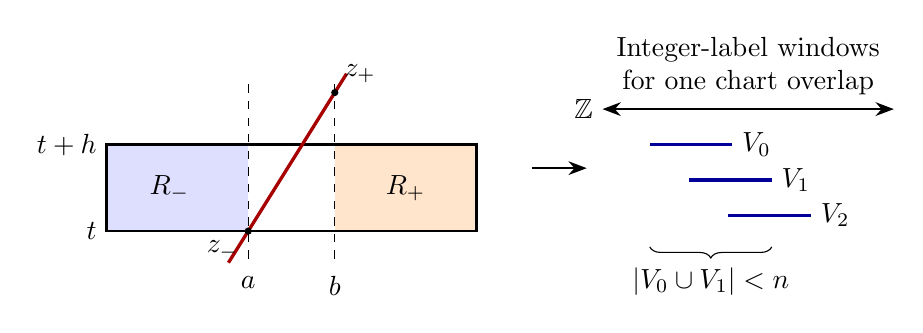
\begin{tikzpicture}[x=1cm,y=1cm,>=Stealth]
 \fill[blue!13] (0.2,0.5) rectangle (2,1.6);
 \fill[orange!20] (3.1,0.5) rectangle (4.9,1.6);
 \draw[thick] (0.2,0.5) rectangle (4.9,1.6);
 \draw[dashed] (2,0.15)--(2,2.4);
 \draw[dashed] (3.1,0.15)--(3.1,2.4);
 \draw[very thick,red!65!black] (1.75,0.1)--(3.25,2.5);
 \fill (2,0.5) circle (1.3pt);
 \fill (3.1,2.26) circle (1.3pt);
 \node[below] at (2,0.05) {$a$};
 \node[below] at (3.1,0.05) {$b$};
 \node at (1,1.05) {$R_-$};
 \node at (4,1.05) {$R_+$};
 \node[left] at (0.2,0.5) {$t$};
 \node[left] at (0.2,1.6) {$t+h$};
 \node[above right] at (3.1,2.26) {$z_+$};
 \node[below left] at (2,0.5) {$z_-$};
 \draw[->,thick] (5.6,1.3)--(6.3,1.3);
 \node[align=center] at (8.35,2.6) {Integer-label windows\\for one chart overlap};
 \draw[<->,thick] (6.5,2.05)--(10.2,2.05);
 \node[left] at (6.5,2.05) {$\ZZ$};
 \draw[very thick,blue!60!black] (7.1,1.6)--(8.15,1.6);
 \draw[very thick,blue!60!black] (7.6,1.15)--(8.65,1.15);
 \draw[very thick,blue!60!black] (8.1,0.7)--(9.15,0.7);
 \node[right] at (8.15,1.6) {$V_0$};
 \node[right] at (8.65,1.15) {$V_1$};
 \node[right] at (9.15,0.7) {$V_2$};
 \draw[decorate,decoration={brace,amplitude=4pt,mirror}]
   (7.1,0.3)--(8.65,0.3);
 \node[below] at (7.875,0.16) {$|V_0\cup V_1|<n$};
\end{tikzpicture}
\caption{The sloping line separates a prefix from a later suffix.
Each geometric overlap receives a separate application of
Lemma~\ref{lem:window-bridge}, starting from the original rectangle.
Within that transfer, short integer windows may leave the source
window; the hull of each consecutive pair, with its fixed margins,
has length less than $n$.  The original extreme endpoint is discarded
in the first enclosure.  The drawing of the slope is schematic.}
\label{fig:propagation-bridge}
\end{figure}

\subsection{Comparing sloping decisions on controlled cells}

We have now established all rectangular laws, without assuming any
joint law for arbitrarily translated sloping predicates.  Consequently
a rectangle and any of its rectangular containers can be compared
exactly, with no restriction on labels.  This removes the quantitative
window issue from the rest of the proof.

\begin{lemma}[Comparison along one line]\label{lem:line-slide}
Let $p$ and $q$ be two chart decisions for the same oriented allowable
sloping line, either primitive charts or charts in the fixed
concurrent templates.  Suppose a point $z$ is on this line, or within
a fixed sufficiently small distance of it, and belongs to the
closures of both chart boxes.  On all sufficiently small rectangular
cells $P$ near $z$ contained in both boxes, $p(s)$ and $q(s)$ have the same
conjugation on every perfect copy controlled in $P$.  The conclusion
also holds when the copies are formal sloping sectors with actual
rectangular control.  Only the rectangular laws and the fixed
geometric tables are used.  At a clipping boundary the comparison is
made on the common interior cells; on exterior cells the decision
from that chart is zero.  Thus a replacement used on both sides must
retain the original clipping condition.
\end{lemma}

\begin{proof}
First suppose the two charts are primitive charts with $\OO^2$
vertices on their common line.  At the first chart use one of the
fixed recentering offsets to obtain an inner chart near $z$.
The first overlap is intersected with the original clipping box.
On a cell on its interior side this is a rectangular container of
$P$.  The fixed comparison table proves equality of the two
decisions on that container.  The same construction is made at
the final chart.  Exterior cells are not an assertion of equality
of the unmasked signs: the original decision is zero by its
actual box-complement law, and a replacement there is clipped
by that same box.

The two recentered $\OO^2$ vertices differ by an element of the
tangent group.  Express this difference in the fixed short basis
and order the signed increments as in the proof of
Proposition~\ref{prop:rectangular-law}.  The centers remain in a
small neighborhood of the segment joining the vertices and hence
near $z$.  More precisely, choose a fixed $\varepsilon>0$ much
smaller than every inner chart margin.  The finite recentering
nets may be chosen to put both endpoints within $\varepsilon/10$
of the tangential projection of $z$, and each basis step may be
chosen shorter than $\varepsilon/10$.  The greedy ordering keeps
every intermediate center within $\varepsilon/2$ of that projection.
If the distance of $z$ from the line and the diameter of $P\cup\{z\}$ are
less than $\varepsilon/10$, every middle overlap therefore has a
fixed positive margin around $P$, independently of the number of
steps and all labels.  The first and last overlaps have the same
margin in their uncut directions; they are simply clipped at the
original box edges.  This supplies a uniform smallness bound,
without shrinking a cell once for each step of a long chain.
All rectangular containers now have their laws by
Proposition~\ref{prop:rectangular-law}, irrespective of their
labels.  Every consecutive fixed table therefore gives equal
actions on a controlled copy by Lemma~\ref{lem:control}.
Their composition gives the desired equality.

For a template with vertex $r+u$, where $u\in\OO^2$, use the
chosen $\OO^2$ anchor on each line of its representative at $r$,
translated by $u$.  The initial and terminal primitive anchors
lie on the same labeled line; their difference is exactly in its
tangent group.  The fixed terminal comparison identifies the
last primitive chart with the template chart.  This accounts
explicitly for vertices in $D^{-1}\OO^2$ without pretending that
the vertex itself is an allowable translation.  A single line
through an arbitrary ordinary point needs only an $\OO^2$
anchor on that line sufficiently close to the point.

At either clipped endpoint every overlap is intersected with
the appropriate inside coordinate half-planes of its box.
These are rectangular conditions with their established law.
Thus the argument applies separately to each actual rectangular
side of the clipping boundary.  It does not require the controlled
copy to split by any intermediate sloping sign.  Its sole use of
the copy is its control in the rectangular overlap.
\end{proof}

\begin{lemma}[One sloping predicate and rectangular partitions]
\label{lem:slope-rectangle}
A translated primitive sloping predicate has a joint central law
with every finite aligned rectangular partition.  At this stage
one may retain both formal sloping sides over each rectangular
cell.  Every resulting perfect copy has the actual rectangular
control of that cell, and hence control in all its rectangular
containers.
\end{lemma}

\begin{proof}
We first compare one sloping predicate $p$ with one translated
primitive coordinate predicate $v$.  Around $p$ choose the fixed
fine rectangular grid included in its initial table.  Include
its clipping edges and its planar chart seams in the grid.
The mesh is chosen smaller than the gaps between the two
boundaries of a primitive coordinate predicate, and sufficiently
small compared with the fixed chart margins and the finitely
many angles.  Translate the whole grid with $p$.

This partition has an actual joint law separately with $p$, by
the fixed table, and with $v$, by the rectangular law.  On one
of its cells $P$, form $H_P$ from the restricted copies of these
two predicates and their complements, as in
Lemma~\ref{lem:patching}.  If either predicate is constant on
$P$, its action on $H_P$ is the indicated constant action.  This
assertion follows from its \emph{individual actual} split with
$P$, together with the conditional move on $P$; it does not use
the pair law being proved.  Only the other individual split is
then needed to check a formal two-predicate relation.

If both predicates vary, $P$ is inside the clipping box of $p$,
one sloping line crosses it, and exactly one boundary line of
$v$ crosses it.  Their intersection is within a fixed multiple
of the diameter of $P$: solve the two line equations, whose
angle is one of a fixed finite list.  It lies in
$D^{-1}\OO^2$.  The grid was chosen fine enough that the
appropriate translated concurrent template has a margin box
containing $P$.  The intersection itself can lie just outside
the clipping box of $p$.  In applying the line comparison choose
instead a point $z_0$ of its sloping line in $\overline P$.
The template intersection is within $C_\lambda\operatorname{diam}P$
of $z_0$, and its chosen $\OO^2$ anchor is within a fixed arbitrarily
small distance of that intersection.  Choose the mesh once so
that this distance and the recentering errors fit the uniform
margin established in Lemma~\ref{lem:line-slide}.  The tangent
walk then stays near $P$ regardless of its number of steps.
No refinement depending on the relative label of $v$ is needed.
Replace $p$ by its corresponding line decision
in that template, using Lemma~\ref{lem:line-slide}, and replace
$v$ by the matching axis decision, using only rectangular
control.  The replacements have exactly the same actions on
$H_P$ as the original generators.

The true template has the four ordinary sectors of these two
crossing lines.  Extend it outside its margin box by any one
of those four assignments.  Therefore a word trivial on all
formal assignments of $(p,v)$ is trivial in this pointwise
template model.  Its lifted value is central in the template
subgroup.  Its rectangular margin box controls every generator
of $H_P$, since it contains $P$ and all rectangular laws are
available.  Take the template law on the enlarged alphabets
required by Lemma~\ref{lem:patching}.  The template-relator
conclusion of that lemma now makes the replacement word act
trivially on $H_P$.

Thus every formal two-predicate relator acts trivially on each
$H_P$.  Lemma~\ref{lem:patching} and then
Lemma~\ref{lem:small-support} prove the pair law.  Apply this
to the coordinate predicates generating any desired rectangular
partition, and apply Lemma~\ref{lem:pair-laws}.  Retain all
exclusions already supplied by the rectangular law.  The
resulting sectors have an actual rectangular cell coordinate,
although their sloping side may still be formal.  Refining by
another rectangle and using the same pair laws proves that
each sector is controlled in every rectangular container of
its cell.  No compatibility of two different sloping predicates
has been used.
\end{proof}

For a finite family $p_1,\ldots,p_k$ and a common rectangular
partition $\mathcal P$, the lemma supplies the separate laws
needed to form the cell groups of Lemma~\ref{lem:patching}:
$H_P$ is generated by all the $p_j$-side factors over $P$.
That lemma makes every $H_P$ invariant under each $p_j(s)$,
so equalities of their actions can be composed before a joint
sloping law is known.  Every generator of $H_P$ is controlled
in $P$ and its rectangular containers, including a generator
assigned a geometrically impossible sloping side.  These are
the groups on which we will verify the actual polygon laws.

\subsection{Actual sectors and clipping boundaries}

The remaining task is to remove those formal extra sides and
prove the joint law for arbitrarily many sloping predicates.
The small rectangular cells are now allowed to depend on the
finite family or word being considered.  The available tables
and the presented group remain fixed.

\begin{lemma}[An inactive line gives a constant action]
\label{lem:inactive-line}
Let $p$ be a translated primitive sloping predicate with clipping
box $B$, and let $z$ be an ordinary point not on its sloping
line $L$.  For sufficiently small rectangular cells $P$ near
$z$ respecting the edges of $B$, the action of $p(s)$ on any
perfect copy controlled in $P$ is its actual constant-side
action inside $B$, and is trivial outside $B$.  The assertion
holds for the formal sector copies of
Lemma~\ref{lem:slope-rectangle}.
\end{lemma}

\begin{proof}
Outside $B$ the actual law of $p$ with its own clipping box
gives the assertion, by exterior rectangular control.
Consider the interior side, allowing $z$ itself to be on an
edge or corner of $B$.  We give the argument for
$L=\{y-\lambda x=c_0\}$; interchange coordinates for the
other slope.  Put $d=z_y-\lambda z_x-c_0\ne0$.

Suppose first that $d>0$.  The point on $L$ with coordinates
\[
 (z_x+d/(2\lambda),\ z_y-d/2)
\]
has $z$ strictly northwest of it.  By density choose
$q_x\in\OO$ within $d/(4\lambda)$ of its first coordinate,
and put $q_y=\lambda q_x+c_0\in\OO$.  Then
\begin{equation}\label{eq:strict-quadrant}
 q_x-z_x>d/(4\lambda),\qquad z_y-q_y>d/4.
\end{equation}
The northwest quadrant based at $q=(q_x,q_y)$ lies wholly on
the positive side of $L$.  For $d<0$, the same formula with
$|d|/(4\lambda)$ as the allowed perturbation puts $z$ strictly
southeast of $q$; that quadrant lies wholly on the negative
side.  Thus the coordinate inequalities have positive room
even when the inactive line is arbitrarily close to $z$.

If $|d|$ is below a fixed small threshold, choose that threshold
so that $q$ and $z$ fit in the inner margins of a line chart.
Lemma~\ref{lem:line-slide} compares the original predicate with
that chart near $z$, clipping the first overlap to $B$.
By \eqref{eq:strict-quadrant}, all sufficiently small cells on
the interior side of $B$ are controlled in the indicated
quadrant and in the chart box.  The genuine line--quadrant
table says that its sign decision there is respectively the
constant permutation or the identity.  Intersection and
transitivity of control give the claimed action on the
controlled copy.  No sign attached to a formal sector was
used to infer its location.

For $|d|$ above the fixed threshold, use the finite rectangular
grid included with the primitive chart.  Choose its mesh small
enough that every cell meeting the part with this lower bound
on $|d|$ lies strictly on the same side of the line.  This is
possible because the defining linear form has fixed norm.
The individual actual table of $p$ with the grid gives its
constant action there.  Rectangular control transfers the
assertion to any sufficiently small $P$ near $z$.  Cells
meeting a grid boundary may be further split by that fixed
grid; this changes neither the conclusion nor the initial
data.

If a clipping edge is active at $z$, treat interior cells by
the quadrant or grid just described and exterior cells by
the first paragraph.  At a corner there are four rectangular
sides and the same procedure applies to each.  Therefore the
local action is exactly the Boolean combination of the
constant sloping sign with the actual clipping decisions on
all sides of the boundary.
\end{proof}

\begin{theorem}[The polygon law]\label{thm:polygon-law}
There is one finite choice of true initial relations in
$\widehat G$, for sufficiently large fixed finite $m$, such
that every finite family of aligned polygon tests has its
actual central law.  The assertion holds simultaneously on
subalphabets.  Its canonical representations
\[
 \rho_{U,I}:\Alt(I)^\ast\longrightarrow\widehat G
\]
are compatible with restriction of the alphabet, split
exactly over finite disjoint polygon refinements, and are
covariant under common translations on proper supports.
\end{theorem}

\begin{proof}
First take a finite family of translated primitive predicates,
including coordinate predicates if needed.  By
Lemma~\ref{lem:small-support}, we may fix an alphabet of its
prescribed bounded size and a word $w$ entirely on that alphabet
whose pointwise permutation is the identity on every actual
assignment.  It suffices to prove that $w$ acts trivially on
the subgroups needed to test centrality.  Include those
additional small-support copies and their spare alphabets
throughout; the geometric family is still finite.

Fix $z\in T$.  Call a supporting boundary line \emph{active}
at $z$ if it contains $z$; include the coordinate lines which
form clipping edges.  Inactive supporting lines have positive
distance from $z$, and the family is finite.  In a sufficiently
small ordinary neighborhood of $z$ the only varying signs are
therefore the active ones.  There is at most one distinct
active line of each of the four directions.

Choose the corresponding translated concurrent template.
If at least two directions are active, $z\in D^{-1}\OO^2$
and the template is provided by its coset representative and
direction subset.  With one active direction use a nearby
$\OO^2$ anchor on that line, and with none use a constant
model.  Each original predicate becomes, in this model, the
Boolean combination of its active sign and clipping decisions,
with the other decisions replaced by their actual local
constants.  The allowed assignments are precisely the
ordinary open sectors of the active lines, with these
combinations evaluated on them.  Each such sector occurs
arbitrarily near $z$ in the original Boolean space.  Hence
the word $w$ is the identity on every assignment of this
template model.  Extend the model outside its margin box
by any one allowed sector, so that it remains a finite
pointwise test model on the whole square.

We verify the equality of its actions with the original
actions on $H_P$ for every sufficiently small cell near $z$.
All cells will be cut by every original clipping edge and
by any additional finite rectangular subdivisions needed
in these comparisons.
\begin{enumerate}[label=(\roman*)]
\item Coordinate decisions compare with the template by
the established rectangular law.  An inactive coordinate
decision is its actual constant on the relevant cells.
\item An active sloping line inside its clipping box
compares with the same oriented line in the template by
Lemma~\ref{lem:line-slide}.  If $z$ lies on a clipping edge,
make that comparison only on the interior rectangular
side.  The template includes that active axis decision,
and its true table identifies the resulting clipped sign
there.  On exterior cells the original predicate is
trivial by control in the exterior of its own box.
This treats all sides of a corner as well.
\item An inactive sloping line is replaced by its actual
constant-side decision by Lemma~\ref{lem:inactive-line}.
If some of its clipping edges are active, keep those
coordinate decisions in the replacement.  The interior
and exterior arguments in that lemma establish precisely
this clipped Boolean combination, even for a formal
wrong-side copy over $P$.
\end{enumerate}
Every equality in this list follows from equal actions on
a known rectangular container of $P$ and the conditional
move of Lemma~\ref{lem:control}.  Thus it holds on every
generator of $H_P$, not just in projection.  The original
generators preserve $H_P$ by Lemma~\ref{lem:patching}.  Their actions
can therefore be composed, and the action of $w$ on $H_P$
equals the action of its template replacement.

The replacement is central in the true template table.
Its margin box is a rectangular container of $P$, so it
controls every generator of $H_P$.  Apply the table on the
enlarged alphabets required by Lemma~\ref{lem:patching}.
The template-relator conclusion of that lemma shows that
the replacement, and hence $w$, centralizes $H_P$, including
its possibly formal sloping factors.

We finally choose one finite partition on which these
local checks all apply.  For every $z$ the preceding
construction provides an ordinary neighborhood and an
upper bound on the permitted cell diameter.  A finite
subcover exists by compactness of $T$.  A sufficiently
fine $\OO$ rectangular grid, refined by the finitely many
clipping edges and auxiliary rectangular cuts of that
subcover, has every cell in one of those neighborhoods
and below its required diameter.  This follows, for
example, by applying the Lebesgue number property to
the finite subcover and then using the coordinate mesh
bound.  Make the separate splits of every original
predicate with this partition by
Lemma~\ref{lem:slope-rectangle}.  We have proved that $w$
centralizes every resulting $H_P$.  The group generated by these
subgroups contains the original test subgroup, so
Lemma~\ref{lem:patching} proves its actual central law.
Lemma~\ref{lem:small-support} gives the assertion on all
the required alphabets simultaneously.

Apply this established law to a larger finite family containing
translated primitive coordinate tests that generate the partition just
used.  Apply Lemma~\ref{lem:law-enlargement} first to the coordinate
subfamily: its original partition copies agree with the corresponding
coordinate factors of the enlarged actual law.  We may therefore include
those same copies among the inputs of that law.  For each old formal law,
the enlarged family now contains exactly its specified input copies,
including the constant copy.  Its subgroup $H_0$ is thus contained in
the enlarged defining-copy subgroup $K$.
Every new actual assignment restricts to an allowed old assignment,
since the old law retained all actual assignments.
Lemma~\ref{lem:law-enlargement} now identifies each \emph{original}
formal factor with the product of its actual refinements and makes it
trivial when it has no actual extension.

Every polygon
is a Boolean combination of finitely many translated
primitive tests.  Apply the law just proved to a common
finite family realizing the polygons.  The canonical
perfect-cover construction supplies their representations.
To compare two Boolean expressions, pass to their common finite
family and apply Lemma~\ref{lem:law-enlargement}; the resulting
representations agree there.  Within this lawful family, uniqueness
of lifts from a perfect source gives exact
multiplicative splitting over a finite disjoint
refinement.  Finally a common allowable translation on
a proper alphabet is implemented by the balanced
translations of Lemma~\ref{lem:translated-copies}; apply
uniqueness to the translated test family.  This proves
the claimed translation covariance and alphabet
compatibility.
\end{proof}

\subsection{Why one finite presentation suffices}

For clarity, we finish by giving the order of the choices used in
this section.  First fix the arithmetic constants and choose
$\lambda$ satisfying \eqref{eq:prop-slope-choice}.  Next choose the
finite concurrent representatives, chart boxes and margins,
quadrant tables, and the fixed grids used away from a line.
Choose the short tangent bases, finite recentering offsets, and
comparison tables inside those margins.  These choices determine
a finite label bound $B$ for every fixed relative configuration,
and a finite constant $K$ for the chart walks in the rectangular
induction.  They also determine all bounded support requirements.
Choose the finite track number $m$ beyond these requirements,
the spare banks of the lifting calculus, and the thresholds
required elsewhere in the argument.

Only now choose $n_0$.  It is large enough for every strict window
inequality, for the rectangles and the separating segment to fit
in the prescribed chart margins, and for
\[
 \frac{9C(\lceil20(K+2)\rceil+1)}{n_0}<\delta.
\]
Enlarge it also for the fixed margins in
\eqref{eq:label-contraction}.  Finally impose the finite true
tables for the coordinate window of length $n_0$ and for the
finite geometric menu, with their specified representative
words and bounded alphabet enlargements.  After common
translations these are exactly the tables used above.

Later induction levels add no initial relation.  Nor does an
arbitrarily close inactive line require a new small geometric
template: its strict quadrant is a translate of a fixed
line--quadrant table, and only the independently controlled
rectangular cell becomes smaller.  Likewise arbitrarily long
words require more cells and more successive comparisons, but
only finitely many tracks at any one comparison.  Thus
Theorem~\ref{thm:polygon-law} is a statement inside a single
finitely presented group $\widehat G$.

\section{Transport of slots and a finitely presented central cover}
\label{sec:transport}

We use the fixed finitely presented group $\widehat G$ and its surjection
$\pi:\widehat G\to A_m$ from Section~\ref{sec:lifting}.  Theorem~\ref{thm:polygon-law}
has established the central law for every finite family of aligned polygon
tests.  Our remaining task is to pass from aligned tests to arbitrary
parameterized slots, including several slots in the same track.  We shall
construct their perfect representations in $\widehat G$, prove exact
conjugation formulas, and deduce that $\ker\pi$ is central.
The first obstacle is that an aligned word can fix every point of a
slot while still using its track.  We handle this with private tracks,
first for distinct-track configurations and then for repeated tracks
by proving independence of the routing.  Translation transport is
proved after that independence is available.

We retain the notation
\[
 B_m=\{d=(d_1,\ldots,d_m)\in\Gamma^m:\textstyle\sum_i d_i=0\},
 \qquad t(d)\in\widehat G,
\]
so that $t(d)t(e)=t(d+e)$ exactly.  Write
$\rho_{P,I}:\Alt(I)^\ast\to\widehat G$ for the canonical representation on
an aligned polygon $P$ and a track set $I$, where $|I|\geq5$.  Its image
is perfect.  These maps split exactly over disjoint polygonal partitions,
are compatible under inclusions of track sets, and obey common-translation
covariance on proper track sets, by Theorem~\ref{thm:polygon-law} and
Lemma~\ref{lem:translated-copies}.  We use function composition in which
$ab$ applies $b$ first.

An \emph{aligned word on $J$} means a finite product of elements of the
images of $\rho_{P,I}$, with $I\subseteq J$.  Such words change track labels
but preserve base coordinates after projection.  Their track support is
$J$: balancing tracks used to write translated predicates in the original
generators are not included in $J$.  This convention is legitimate because
Lemma~\ref{lem:translated-copies} proves exact commutation for disjoint
track sets, independently of those choices of balancing words.  In
particular, $t(d)$ commutes with every aligned word on $J$ if $d_i=0$ for
all $i\in J$.

For a finite family with its actual central law, the restriction of
$\pi$ to the subgroup $H$ of conditional copies maps onto the
pointwise group on its nonempty Boolean atoms.  That pointwise group
is a product of alternating groups and acts faithfully on $mX$.
Thus every word in the kernel evaluates to the identity in the actual
assignment model, and the actual central law makes this kernel central.
This supplies the central extensions used below.

Here is the elementary consequence of perfection that will repeatedly
turn a central law into an exact identity.  If $H\to Q$ has central kernel,
$K\leq H$ is perfect, and the image of $b\in H$ centralizes the image of
$K$, then $[b,k]$ is central for every $k\in K$.  The map
$k\mapsto[b,k]$ is therefore a homomorphism from $K$ to an abelian group,
and is trivial.  Thus $b$ centralizes $K$ exactly.  Also, two homomorphisms
from a perfect group to $H$ with the same composition into $Q$ are equal.
Every application below takes place in a specified finite test subgroup
with this central-extension property.

\subsection{Offset frames and distinct tracks}

A parameterized five-slot configuration is data
\begin{equation}
 S=(U;(i_1,u_1),\ldots,(i_5,u_5)),
 \qquad U\subseteq X,\quad i_j\in\{1,\ldots,m\},\quad u_j\in\Gamma,
 \label{eq:slot-configuration}
\end{equation}
where $U$ is a Boolean polygon and the five images of the maps
\[
 s_j:U\longrightarrow mX,\qquad s_j(x)=(i_j,x+u_j)
\]
are pairwise disjoint.  Addition is modulo the coordinate periods, with
the induced action on $X$.  Thus equal track indices are allowed precisely
when the corresponding translated pieces are disjoint.  The ordering
identifies slot permutations with
$E=\Alt(\{1,\ldots,5\})$.  All representations associated to five-slot
configurations will have the same source $E^\ast$.  For an empty $U$ the
representation is the trivial one, and empty pieces in refinements will
be omitted.

For a proper track set $J$ and offsets $a_i\in\Gamma$ for $i\in J$, choose
$f\in B_m$ with $f_i=a_i$ on $J$.  Such an $f$ exists by balancing the sum
on one track outside $J$.  Conjugating aligned representations on $J$ by
$t(f)$ gives their representations in the \emph{offset frame} $a$.  The
choice of $f$ has no effect: if $f'$ is another choice, then $f'-f$ vanishes
on $J$ and $t(f'-f)$ commutes with every aligned word there.  Every finite
central law on $J$ consequently gives the same central law in this frame.

Suppose first that the $i_j$ in~\eqref{eq:slot-configuration} are distinct.
Put $I=\{i_1,\ldots,i_5\}$, let
$\iota_{\boldsymbol i}^\ast:E^\ast\to\Alt(I)^\ast$ be the isomorphism
induced by $j\mapsto i_j$, and choose $f\in B_m$ with $f_{i_j}=u_j$.
Define
\begin{equation}
 \rho_S(s)=t(f)\rho_{U,I}(\iota_{\boldsymbol i}^\ast(s))t(f)^{-1},
 \qquad s\in E^\ast.
 \label{eq:distinct-slot-copy}
\end{equation}
This is independent of the balancing coordinates of $f$, and its
projection is the indicated alternating slot permutation.

\begin{lemma}[Compatibility of frames]\label{lem:slot-frames}
For distinct-track configurations, the representations
\eqref{eq:distinct-slot-copy} have the following properties.
\begin{enumerate}[label=\textup{(\roman*)}]
\item Replacing $U$ by $U+v$ and every $u_j$ by $u_j-v$ leaves the
representation unchanged, with the corresponding reparameterization.
\item If $U=\bigsqcup_{\alpha=1}^r U_\alpha$, then
\begin{equation}
 \rho_S(s)=\prod_{\alpha=1}^r\rho_{S|U_\alpha}(s),
 \label{eq:slot-refinement-distinct}
\end{equation}
and the factor images commute pairwise.
\item For a constant even track permutation $c$, conjugation by its fixed
lift sends $\rho_S$ to the representation of the tuple obtained by
replacing $i_j$ by $c(i_j)$.
\item For every $d\in B_m$,
\begin{equation}
 t(d)\rho_S(s)t(d)^{-1}=\rho_{dS}(s),
 \qquad
 dS=(U;(i_j,u_j+d_{i_j})_{j=1}^5).
 \label{eq:distinct-translation}
\end{equation}
\end{enumerate}
More generally, a representation on a subalphabet computed in an offset
frame agrees with its own frame definition.  Two frames giving the same
offsets on that subalphabet, up to the common reparameterization in
\textup{(i)}, give identical representations there.
\end{lemma}

\begin{proof}
For (i), choose $h\in B_m$ equal to $v$ on $I$.  The common-translation
identity for aligned copies is
$t(h)\rho_{U,I}t(h)^{-1}=\rho_{U+v,I}$.  A balancing vector for the new
offsets, added to $h$, agrees with $f$ on $I$.  Independence of the balance
then proves the assertion.  Part (ii) is the aligned refinement identity
conjugated by $t(f)$.

For (iii), the initial relations give
$c\,t(f)c^{-1}=t(c\cdot f)$ and exact reindexing of the aligned
representations.  These are precisely the data defining the new frame.
For (iv), additivity gives
\[
 t(d)\rho_S(s)t(d)^{-1}
 =t(d+f)\rho_{U,I}(\iota_{\boldsymbol i}^\ast(s))t(d+f)^{-1};
\]
$d+f$ has the required offsets on $I$.  Finally, compatibility under
restriction follows from the corresponding compatibility of aligned
canonical representations and from independence of balances.  This also
proves the assertion about two frames.
\end{proof}

We next prove transport by aligned words.  Private track blocks move
the entire representation away from a word fixing its slots without
changing the commutator.  The lemmas state the spare-track hypotheses
for the indicated support of that word.  Their later applications
compare bounded unions of supports; the final kernel word is treated
one generator at a time.

\begin{lemma}[Fixing a distinct-track tuple]\label{lem:fixed-slot-centralizer}
Let $S$ be a five-slot configuration on distinct tracks, and let $b$ be
an aligned word on a track set $J$.  Suppose that $\pi(b)$ fixes every
point of every parameterized slot of $S$.  Provided the fixed track
reserve contains twenty tracks outside $J$ and the occupied tracks,
together with the balancing tracks used below, $b$ centralizes
$\rho_S(E^\ast)$ exactly.
\end{lemma}

\begin{proof}
For each leg $j$, choose four private tracks
$p_{j,1},\ldots,p_{j,4}$, all distinct and outside $J\cup I$, and put
\[
 V_j=U+u_j,
 \qquad L_j=\{i_j,p_{j,1},\ldots,p_{j,4}\},
 \qquad K_j=\rho_{V_j,L_j}(\Alt(L_j)^\ast).
\]
The projected element $\pi(b)$ fixes the source track pointwise on $V_j$
and fixes every private track.  It therefore commutes with the projection
of $K_j$.  Take the finite family consisting of all tests occurring in a
chosen aligned expression for $b$, the five tests $V_j$, and constants,
on the union of the track sets involved.  Theorem~\ref{thm:polygon-law}
gives a central extension of its pointwise group.  Within that subgroup,
$[b,k]$ is central for $k\in K_j$.  Since $K_j$ is perfect, the
central-commutator argument above proves
\begin{equation}
 [b,K_j]=1\qquad (1\leq j\leq5).
 \label{eq:fixer-private-commutation}
\end{equation}

Choose $a_j\in K_j$ projecting to the cycle
$(i_j\ p_{j,1}\ p_{j,2})$ on $V_j$, and set $a=a_5\cdots a_1$.
There is one common offset frame on the union of the $L_j$: assign offset
$u_j$ to every track in $L_j$.  In this frame, $K_j$ is the aligned
conditional copy on $U$ with track set $L_j$.  Thus $a$ and $\rho_S$ lie
in one conjugate of a subgroup with an aligned central law.  In its
pointwise model, $a$ sends the $j$th slot to
$(p_{j,1},U+u_j)$.  Uniqueness for homomorphisms from $E^\ast$ in this
central extension gives the exact identity
\begin{equation}
 a\rho_S(s)a^{-1}=\rho_T(s),
 \qquad T=(U;(p_{j,1},u_j)_{j=1}^5).
 \label{eq:private-evacuation}
\end{equation}
Here compatibility of subframes in Lemma~\ref{lem:slot-frames} identifies
the two maps with their definitions in~\eqref{eq:distinct-slot-copy}.

The tracks occupied by $T$ are outside $J$.  Write its representation
using a balancing vector $f_T$ which is zero on $J$: prescribe $u_j$ on
$p_{j,1}$ and balance on a further track outside both sets.  The aligned
base copy for $T$ commutes with $b$ by disjoint-track commutation, and
$t(f_T)$ commutes with $b$ because $f_T$ vanishes on $J$.  Consequently
$[b,\rho_T(E^\ast)]=1$.  Equation~\eqref{eq:fixer-private-commutation}
also gives $[b,a]=1$.  Conjugating~\eqref{eq:private-evacuation} back proves
$[b,\rho_S(E^\ast)]=1$.
\end{proof}

\begin{lemma}[Aligned transport between distinct-track tuples]
\label{lem:distinct-slot-transport}
Let $S=(U;(i_j,u_j)_{j=1}^5)$ and
$T=(U;(k_j,u_j)_{j=1}^5)$ be configurations, each with distinct track
indices.  If an aligned word $b$ sends the $j$th parameterized slot of
$S$ to the $j$th slot of $T$, then
\begin{equation}
 b\rho_S(s)b^{-1}=\rho_T(s)\qquad(s\in E^\ast),
 \label{eq:distinct-aligned-transport}
\end{equation}
whenever the fixed reserve supplies the tracks of
Lemma~\ref{lem:fixed-slot-centralizer} for $b$ and an even constant
reindexing of the two tuples.
\end{lemma}

\begin{proof}
Extend the bijection $i_j\mapsto k_j$ to a permutation of the union of
the two five-element sets.  If it is odd, multiply by a transposition on
two additional tracks.  The resulting even constant permutation $c$
has support at most twelve and sends $S$ to $T$ parameterwise.
The aligned word $c^{-1}b$ fixes $S$ pointwise.  Apply
Lemma~\ref{lem:fixed-slot-centralizer}, and then the constant-reindexing
identity of Lemma~\ref{lem:slot-frames}.
\end{proof}

\subsection{Repeated tracks and independence of routing}

We now construct the representation of~\eqref{eq:slot-configuration}
without a distinctness assumption on the $i_j$.  An \emph{admissible
routing} of $S$ is an aligned word $r$ on an alphabet of at most
$25$ tracks containing all source and terminal track labels, whose
projected action sends its five slots parameterwise to a tuple $T$ on
distinct tracks.  Since an aligned word preserves base
coordinates, $T$ has the form $(U;(k_j,u_j)_{j=1}^5)$.  A routing need not
act trivially outside the specified slots; this is useful when the same
routing is applied to a subdivision of $U$.

Such a routing always exists.  Choose four private tracks for each leg,
all outside the occupied source tracks and all different.  On
$V_j=U+u_j$ choose an element of the perfect aligned copy on
\[
 L_j=\{i_j,p_{j,1},p_{j,2},p_{j,3},p_{j,4}\}
\]
projecting to $(i_j\ p_{j,1}\ p_{j,2})$.  Multiply these five elements
to obtain $r$.  Each factor sends its own slot to $p_{j,1}$.  It fixes
every other source slot: different source tracks are not in its private
block, and slots sharing $i_j$ have disjoint Boolean regions by
hypothesis.  Private destinations of different legs are distinct.
The total support is at most $5+5\cdot4=25$.

For an admissible routing $r:S\to T$, define provisionally
\begin{equation}
 \rho_S^{\,r}(s)=r^{-1}\rho_T(s)r.
 \label{eq:routed-copy}
\end{equation}
The next lemma proves equality of these maps in $\widehat G$ itself.

\begin{lemma}[Independence of routing]\label{lem:routing-independence}
For every five-slot configuration $S$, the homomorphism
\eqref{eq:routed-copy} is independent of its admissible routing.  Denote
it by $\rho_S:E^\ast\to\widehat G$.  It agrees with
\eqref{eq:distinct-slot-copy} when the tracks are distinct.  For every
finite polygonal partition $U=\bigsqcup_\alpha U_\alpha$,
\begin{equation}
 \rho_S(s)=\prod_\alpha\rho_{S|U_\alpha}(s),
 \label{eq:slot-refinement}
\end{equation}
with pairwise commuting factor images.  Common reparameterization of
$U$ and the $u_j$ leaves $\rho_S$ unchanged.
\end{lemma}

\begin{proof}
Let $r_1:S\to T_1$ and $r_2:S\to T_2$ be two admissible routings.  The
aligned word $b=r_2r_1^{-1}$ sends $T_1$ to $T_2$ parameterwise.  Both
terminal tuples have distinct tracks, so Lemma~\ref{lem:distinct-slot-transport}
applies and gives
\[
 r_2r_1^{-1}\rho_{T_1}(s)r_1r_2^{-1}=\rho_{T_2}(s).
\]
After multiplying by $r_2^{-1}$ and $r_2$, this is precisely
$\rho_S^{\,r_1}(s)=\rho_S^{\,r_2}(s)$.  A distinct-track tuple admits the
identity routing, proving agreement with its earlier definition.

Fix one routing $r:S\to T$.  It is also an admissible routing of every
$S|U_\alpha$ to $T|U_\alpha$: its support bound has not changed.  Apply
Lemma~\ref{lem:slot-frames}(ii) to $T$, and conjugate the identity and its
commutation assertions by $r^{-1}$.  This proves~\eqref{eq:slot-refinement}.
For common reparameterization, use the same routing, which depends only
on the actual parameterized slot maps after their domain identification,
and apply Lemma~\ref{lem:slot-frames}(i) at its distinct-track target.
\end{proof}

Routing independence has now been established using aligned words only.
In particular, it is available before any claim that a translation
transports a repeated-track configuration.

\begin{lemma}[Aligned transport of arbitrary tuples]
\label{lem:aligned-slot-transport}
Let $b$ be an aligned word supported on at most five tracks.  Suppose
that it sends a five-slot configuration $S$ parameterwise to a
configuration $T$ with constant track labels on each leg.  Then
\begin{equation}
 b\rho_S(s)b^{-1}=\rho_T(s)\qquad(s\in E^\ast).
 \label{eq:aligned-slot-transport}
\end{equation}
If track labels vary within $U$, the same assertion holds piecewise on
a finite polygonal partition of $U$, with the product interpretation
of~\eqref{eq:slot-refinement}.
\end{lemma}

\begin{proof}
Choose admissible routings $r_S:S\to S'$ and $r_T:T\to T'$.  The word
$r_Tbr_S^{-1}$ is aligned and sends the distinct-track tuple $S'$ to
$T'$.  Lemma~\ref{lem:distinct-slot-transport} gives
\[
 (r_Tbr_S^{-1})\rho_{S'}(s)(r_Tbr_S^{-1})^{-1}=\rho_{T'}(s).
\]
Conjugate by $r_T^{-1}$ and use the definitions of $\rho_S$ and $\rho_T$.
The support of the transition word is at most $25+5+25=55$, so this
application uses a fixed reserve.

For the last assertion, the finitely many polygon tests in $b$ induce
a finite partition on each map $x\mapsto x+u_j$.  Their common refinement
makes all five terminal track labels constant.  Apply the proved
identity on every part and multiply, using~\eqref{eq:slot-refinement}.
\end{proof}

\subsection{Balanced translations}

The representations on repeated tracks are now independent of routing.
We next use that independence to prove translation covariance.  The
auxiliary translation below shifts each chosen routing block uniformly;
a second routing handles the difference from the desired translation.

\begin{lemma}[Translation transport]\label{lem:translation-slot-transport}
For every $d\in B_m$ and every five-slot configuration $S$,
\begin{equation}
 t(d)\rho_S(s)t(d)^{-1}=\rho_{dS}(s),
 \qquad s\in E^\ast,
 \label{eq:translation-slot-transport}
\end{equation}
where $dS=(U;(i_j,u_j+d_{i_j})_{j=1}^5)$.
\end{lemma}

\begin{proof}
It suffices to treat the fixed generators of $B_m$, each supported on
two tracks, and their inverses.  The general statement then follows by
composition and additivity of $t$.

Choose the private-block routing $r:S\to T$ used in the existence proof
above.  Its $j$th factor lies in $\rho_{V_j,L_j}(\Alt(L_j)^\ast)$, where
$V_j=U+u_j$.  Choose $d'\in B_m$ as follows:
\begin{equation}
 d'_i=d_i\quad\text{on every occupied source track }i,
 \qquad d'_{p_{j,a}}=d_{i_j}\quad(1\leq j\leq5,\ 1\leq a\leq4).
 \label{eq:blockwise-translation}
\end{equation}
Put $d'=0$ on the other tracks except for one unused track, on which
we balance the sum.  Repeated source labels give consistent prescriptions
because they prescribe the same $d_i$.  Thus $d'$ is constant on each
$L_j$, and has support at most $26$.  Set
\[
 \delta=d-d'.
\]
The translation $\delta$ vanishes on all occupied source tracks and has
bounded support (at most $28$ is sufficient).

We first show
\begin{equation}
 [t(\delta),\rho_S(E^\ast)]=1.
 \label{eq:delta-centralizes}
\end{equation}
Choose another private-block routing $q:S\to T_0$, with all its private
tracks outside the support of $\delta$.  Every track in each of its
five blocks then has $\delta_i=0$.  Outside-support translation
commutation, from Lemma~\ref{lem:translated-copies}, gives
$[t(\delta),q]=1$ factor by factor.  The tuple $T_0$ has distinct tracks,
all outside the support of $\delta$.  Write
\[
 \rho_{T_0}(s)=t(f)\rho_{U,I_0}
       (\iota_{\boldsymbol k}^\ast(s))t(f)^{-1}.
\]
The element $t(\delta)$ commutes with $t(f)$ by additivity and with the
aligned representation on $I_0$ because it is zero on $I_0$.
It therefore centralizes $\rho_{T_0}(E^\ast)$.  By the already proved
routing independence,
$\rho_S=q^{-1}\rho_{T_0}q$, proving~\eqref{eq:delta-centralizes}.
This argument uses only the distinct-track frame formula and
outside-support commutation.

Next conjugate the original routing by $t(d')$.  Since $d'$ is constant
on $L_j$, the common-translation law for aligned polygon representations
replaces its $j$th conditional factor on $V_j$ by the same factor on
$V_j+d_{i_j}$.  Hence
\[
 r'=t(d')rt(d')^{-1}
\]
is an aligned word on the same at-most-$25$ tracks.  It routes $d'S$
to $d'T$, preserving base coordinates at this new configuration.  It is
therefore an admissible routing.  The distinct-track formula
\eqref{eq:distinct-translation} gives
\[
 \begin{split}
 t(d')\rho_S(s)t(d')^{-1}
 &=r'^{-1}\bigl(t(d')\rho_T(s)t(d')^{-1}\bigr)r'\\
 &=r'^{-1}\rho_{d'T}(s)r'
 =\rho_{d'S}(s).
 \end{split}
\]
Finally, $d'S=dS$ because $d'=d$ on the occupied source tracks, while
$t(d)=t(d')t(\delta)$.  Equation~\eqref{eq:delta-centralizes} now proves
\eqref{eq:translation-slot-transport}.
\end{proof}

\paragraph{The fixed number of tracks.}
We record why the preceding constructions fit the single choice of $m$
made before the presentation was fixed.  One private routing uses at most
$25$ tracks.  Comparing two routings uses at most $50$, and inserting one
five-track aligned generator uses at most $55$.  The even constant
reindexing in Lemma~\ref{lem:distinct-slot-transport} uses at most twelve
tracks.  The fixing-slot argument adds twenty private tracks and finitely
many balancing tracks.  The translation argument uses the source tracks,
two banks of twenty private tracks, the at-most-two-track support of its
generator, and a balancing track; its temporary difference translation
has support at most $28$.  These are absolute finite bounds, independent
of polygons, offsets, the number of refinement pieces, and word length.
Let $M_{\mathrm{tr}}$ be the maximum of the total track requirements
of these finitely many operations, including the auxiliary tracks in
each.  Taking $m>M_{\mathrm{tr}}$ in addition to the earlier support
requirements makes every comparison available.

A refined piece uses the same routing as its parent.  Different pieces
are processed successively, and successive word letters may reuse the
private banks because Lemma~\ref{lem:routing-independence} identifies all
choices exactly.  No bank is assigned permanently to a predicate, a
refinement level, or a letter of a later word.  The only relations used
here are the initial additive and reindexing relations, outside-support
commutation, and the polygon laws already deduced in the fixed presented
group.  In particular, this reserve does not require any new relations
depending on the configuration being transported.

\subsection{Generation and centrality of the kernel}

Let $N\leq\widehat G$ be the subgroup generated by
$\rho_S(E^\ast)$ over all parameterized five-slot configurations $S$.
We first check that these copies generate the presented group itself.
This is stronger than their generation after projection and is necessary
for the kernel argument.

\begin{lemma}[Generation by slot copies]\label{lem:slot-generation}
The subgroup $N$ is all of $\widehat G$.
\end{lemma}

\begin{proof}
Each of the initial conditional alternating track groups is generated
by its subgroups on five tracks.  The canonical representations on those
five tracks agree exactly with their initially specified lifts, by the
finite initial tables and uniqueness for perfect sources.  Thus $N$
contains all conditional track-permutation generators, including the
constant ones.

It remains to include the balanced translation generators.  Let $v$ be
one of the two fixed generators of $\Gamma$, and choose four distinct
tracks $i,j,k,h$.  Put
\[
 c=(i\ j\ k),\qquad a=v e_i-v e_h\in B_m,
\]
where $e_i$ denotes placement in the $i$th track coordinate.  We use the
same symbol $c$ for the specified constant lift.  The additive and
constant-reindexing relations give
\begin{equation}
 [c,t(a)]=t(c\cdot a-a)=t(v e_j-v e_i).
 \label{eq:translation-as-slot-product}
\end{equation}
The commutator convention is $[x,y]=xyx^{-1}y^{-1}$.  On the other hand,
\[
 [c,t(a)]=c\,\bigl(t(a)c^{-1}t(a)^{-1}\bigr).
\]
The first factor belongs to a constant five-track representation, after
adjoining two track labels to the three moved by $c$.  The second belongs
to its offset-frame conjugate and hence, by
\eqref{eq:distinct-slot-copy}, to another five-slot representation.
Both factors are in $N$, so $t(v e_j-v e_i)\in N$.

Such differences generate $B_m$.  Only the fixed basis differences
are needed for the finite generator list, and the finitely many instances
of~\eqref{eq:translation-as-slot-product} are among the initial relations
of Section~\ref{sec:lifting} (they also follow from its additive and
reindexing relations).  This proves $N=\widehat G$ without assuming that
any conjugating translation already belongs to $N$.
\end{proof}

\begin{theorem}[A finitely presented central cover]\label{thm:central-cover}
For all sufficiently large fixed finite $m$, there is a finitely
presented group $\widehat G$ and a surjective homomorphism
$\pi:\widehat G\to A_m$ whose kernel is central.
\end{theorem}

\begin{proof}
Choose $m$ beyond the fixed track requirements of the lifting and
propagation arguments and $M_{\mathrm{tr}}$.  Choose the
finite initial relation menu in the order specified in
Sections~\ref{sec:lifting} and~\ref{sec:propagation}.  This produces the
finitely presented group $\widehat G$ and the surjection $\pi$; the
transport lemmas have all been proved inside this group.

Take $w\in\ker\pi$, and write it as a finite word in the chosen
generators and their inverses.  Each conditional permutation letter
can be written, using its initial finite group table, as a product of
letters supported on five tracks.  Thus we may regard every letter
as either a five-track aligned element or a fixed balanced translation
generator or its inverse.  Write the resulting word as $w=g_n\cdots g_1$
and put $w_k=g_k\cdots g_1$, so that the letters act in the order
$g_1,\ldots,g_n$.  Fix a configuration
$S=(U;(i_j,u_j)_{j=1}^5)$.

There is a finite polygonal partition $U=\bigsqcup_\alpha U_\alpha$
such that, along every $w_k$ and for each of the five
legs, its image on $U_\alpha$ has one fixed track label and one fixed
translation offset.  To construct the partition, pull back the finitely
many continuity pieces of each next letter along the five current
partial translations and intersect with the pieces already obtained.
The Boolean algebra is closed under these operations.  Induction on
the finite word length therefore gives a finite partition; there is no
claimed bound on its number of pieces.

On a nonempty $U_\alpha$, follow the resulting five-slot tuple through
successive letters.  The images remain disjoint because every projected
letter is a bijection.  Lemma~\ref{lem:aligned-slot-transport} applies
to aligned letters and Lemma~\ref{lem:translation-slot-transport} to
translation letters.  Composing their exact conjugation identities
gives
\begin{equation}
 w\rho_{S|U_\alpha}(s)w^{-1}
   =\rho_{\pi(w)(S|U_\alpha)}(s).
 \label{eq:word-slot-transport}
\end{equation}
Since $\pi(w)=1$, the terminal tuple equals the initial tuple
parameterwise.  In particular the terminal track labels are the same;
the terminal offsets are the same in $\Gamma$, since the translation
action on $X$ is free.  The right side of~\eqref{eq:word-slot-transport}
is consequently $\rho_{S|U_\alpha}(s)$.

Multiply these identities over $\alpha$ and use the exact refinement
formula~\eqref{eq:slot-refinement}.  We obtain
$[w,\rho_S(E^\ast)]=1$ for every configuration $S$.
Lemma~\ref{lem:slot-generation} says that these images generate
$\widehat G$, so $w\in Z(\widehat G)$.  Since $w$ was arbitrary,
$\ker\pi\subseteq Z(\widehat G)$, as required.
\end{proof}

\section{Finite presentation and the main theorem}\label{sec:conclusion}

We now combine the two finiteness statements. Their separation is
useful: finite generation of a Schur multiplier alone would not
give finite presentation.

\begin{lemma}\label{lem:kill-central-kernel}
Let $G$ be a group with finitely generated $H_2(G;\ZZ)$.
If there is a central extension
\[
 1\longrightarrow K\longrightarrow E\longrightarrow G
 \longrightarrow1
\]
with $E$ finitely presented, then $G$ is finitely presented.
\end{lemma}

\begin{proof}
The five-term exact sequence in integral group homology for this
extension \cite[6.8.3, p.~196]{Weibel1994} gives
\[
 H_2(E;\ZZ)\longrightarrow H_2(G;\ZZ)
 \longrightarrow K\longrightarrow E_{\mathrm{ab}}
 \longrightarrow G_{\mathrm{ab}}\longrightarrow0.
\]
Here the usual coinvariant term $K/[E,K]$ is $K$ because the kernel
is central. The image of $H_2(G;\ZZ)$ is a finitely generated
abelian subgroup of $K$. Its quotient in $K$ embeds in the finitely
generated abelian group $E_{\mathrm{ab}}$, and hence is finitely
generated as well. Thus $K$ is finitely generated abelian.
Choose generators $k_1,\ldots,k_s$ and represent them by words in a
finite presentation of $E$. Adding these $s$ words as relators
presents $E/K\cong G$, since a central subgroup generated by these
elements is also their normal closure.
\end{proof}

\begin{proof}[Proof of Theorem~\ref{thm:main}]
Choose $\lambda$ as in \eqref{eq:lambda-choice}. Then choose a
finite number $m$ of tracks large enough for both
Theorem~\ref{thm:multiplier} and Theorem~\ref{thm:central-cover},
including the fixed reserves used in the latter. These are finitely
many requirements on $m$; none depends on the length of a later
word or the size of a later polygon partition.

Set $G=A_m$. Theorem~\ref{thm:simplicity} makes $G$ infinite,
perfect, and simple. Theorem~\ref{thm:amenability} makes $F_m$
amenable, and the subgroup passage proved there makes $G$ amenable
in the stated F\o lner sense. Theorem~\ref{thm:multiplier} gives
finite generation of $H_2(G;\ZZ)$, while
Theorem~\ref{thm:central-cover} gives a finitely presented central
extension of $G$. Lemma~\ref{lem:kill-central-kernel} now proves
that $G$ is finitely presented. These are all the required
properties.
\end{proof}

\clearpage
\begingroup
\raggedright
\bibliographystyle{plain}
\bibliography{references/literature}
\endgroup
\end{document}
